\appendix

\chapter{Comparaciones por Género}\label{ApendiceA}

%%%%%%%%%%%%%%%%%%%%%%%%%%%%%%%%%%%%%%%%%%%%%%%%%%%%%%
%%%%%%% A N A L I S I S  P O R  G E N E R O %%%%%%%%%%
%%%%%%%%%%%%%%%%%%%%%%%%%%%%%%%%%%%%%%%%%%%%%%%%%%%%%%



\subsection{Boxplot Funcionales por Género}

A continuación se presenta un análisis detallado de las curvas de glucosa e insulina por género. En la Figura \ref{fig:glucosaNormal}, se muestra una comparación de los boxplots funcionales entre hombres y mujeres de individuos cuyo prediagnóstico es normal. En la curva mediana de ambos boxplots, se observa una tendencia creciente seguida de un descenso. Sin embargo, en la curva mediana asociada a hombres, el pico se alcanza a los $30$ minutos y luego desciende, mientras que en las mujeres, el pico parece estar entre los $30$ y $60$ minutos antes de descender. Este comportamiento también se observa en la curva del tercer cuartil.

Adicionalmente, en las curvas asociadas al primer cuartil en ambos casos, se observa un descenso seguido de un ascenso, lo que sugiere posibles errores de medición.

\begin{figure}[H]
 \centering
  \subfloat[Mujeres]{
   \label{bfMuGluNormal}
    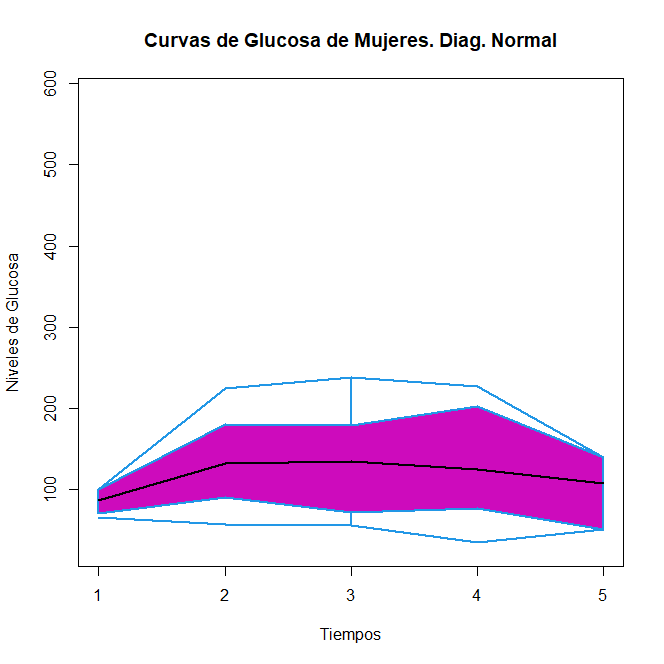
\includegraphics[width=0.45\textwidth]{img/bfMujgluNormal.png}}
  \subfloat[Hombres]{
   \label{bfHoGluNormal}
    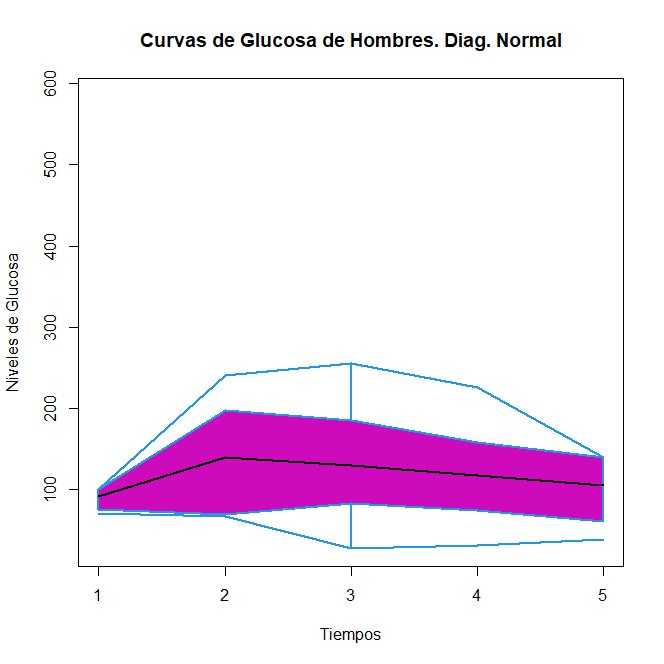
\includegraphics[width=0.45\textwidth]{img/bfHogluNormal.png}}
    \caption{Boxplot funcional para las curvas de glucosa para personas con prediagnóstico normal.}
    \label{fig:glucosaNormal}
\end{figure}


Los boxplots correspondientes a las curvas de insulina de la Figura \ref{fig:insulinaNormal}, muestran un comportamiento similar en ambos géneros, con una curva mediana ascendente seguida de un descenso, aunque en el caso de los hombres esta curva parece ser más pronunciada.

Es importante destacar que en el boxplot correspondiente a mujeres se observan varios outliers, con niveles de insulina bastante altos. Esto sugiere la posibilidad de que estos individuos estén experimentando resistencia a la insulina, aunque esta condición aún no se refleje claramente en su curva de insulina. Por otro lado, la curva del primer cuartil muestra niveles bajos en ambos casos.

En cuanto al tercer cuartil, la curva de las mujeres se asemeja bastante a la curva correspondiente a la mediana, lo que sugiere una forma común. Sin embargo, en los hombres esta curva se modifica ligeramente posiblemente algún error de medición.


\begin{figure}[H]
 \centering
  \subfloat[Mujeres]{
   \label{bfMuGluInsulina}
    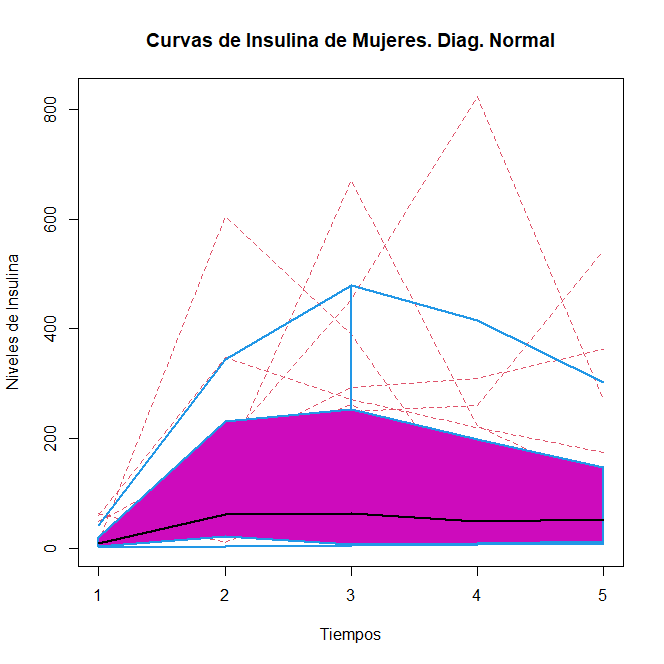
\includegraphics[width=0.45\textwidth]{img/bfMuInsNormal.png}}
  \subfloat[Hombres]{
   \label{bfHoGluInsulina}
    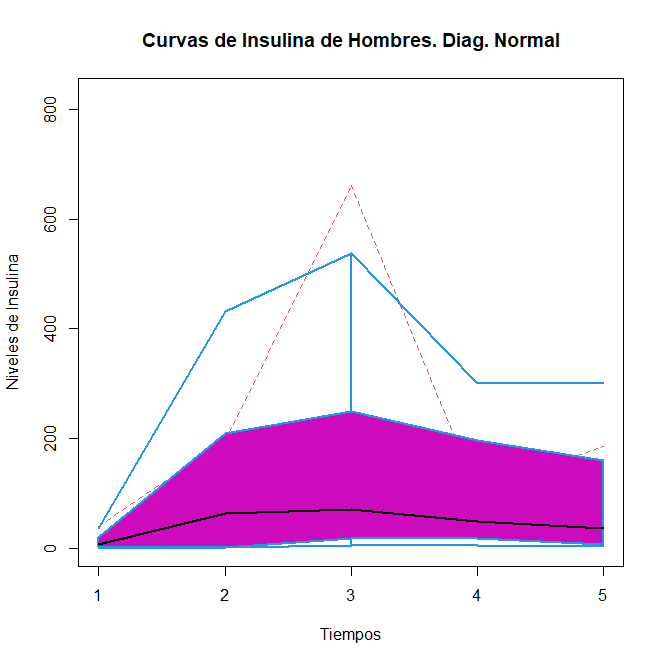
\includegraphics[width=0.45\textwidth]{img/bfHoInsNormal.png}}
    \caption{Boxplot funcional para las curvas de insulina para personas con prediagnóstico normal.}
    \label{fig:insulinaNormal}
\end{figure}





%%%%%%%%%%%%%%%%%%%%%%%%%%%%%%%%%%%%%%%%%%%%%%%%%%%%%%%%

En la nueva categoría de prediabéticos, los boxplots funcionales de glucosa para hombres y mujeres muestran diferencias significativas. La curva mediana en mujeres es ascendente hasta el minuto $90$ y luego comienza a descender, mientras que en hombres alcanza su máximo a los $60$ minutos. El tercer cuartil presenta un comportamiento similar, aunque en mujeres parece haber una mayor resistencia a la insulina, ya que los valores de glucosa no disminuyen tanto.

La curva del primer cuartil correspondientes a hombres y mujeres muestra nuevamente un patrón ascendente, descendente y posteriormente ascendente, lo que podría sugerir otro posible error de medición. Por otro lado, la curva del bigote inferior de mujeres parece seguir la misma forma que la curva mediana de mujeres, lo que sugiere una tendencia común en este grupo.

Adicionalmente, a los $120$ minutos, los valores de las curvas de glucosa de las mujeres tienen una varianza mucho mayor que los de los hombres.

\begin{figure}[H]
 \centering
  \subfloat[Mujeres]{
   \label{bfMuGluPredia}
    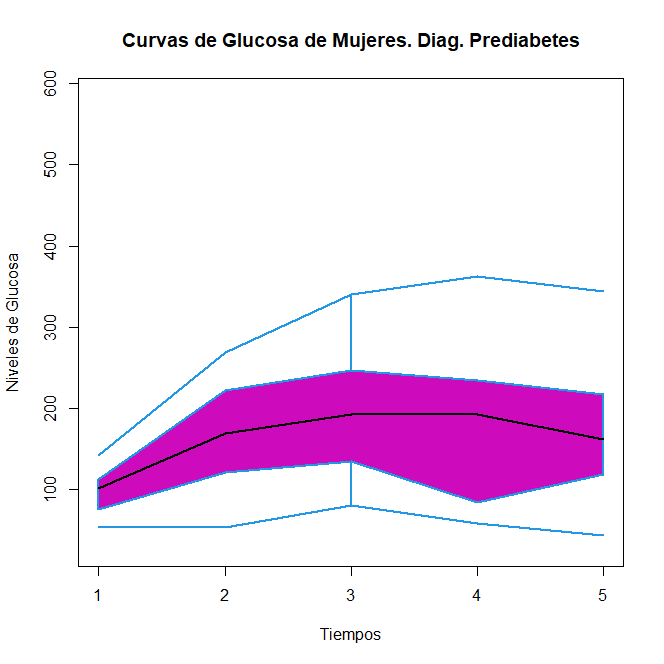
\includegraphics[width=0.45\textwidth]{img/bfMugluPredia.png}}
  \subfloat[Hombres]{
   \label{bfHoGluPredia}
    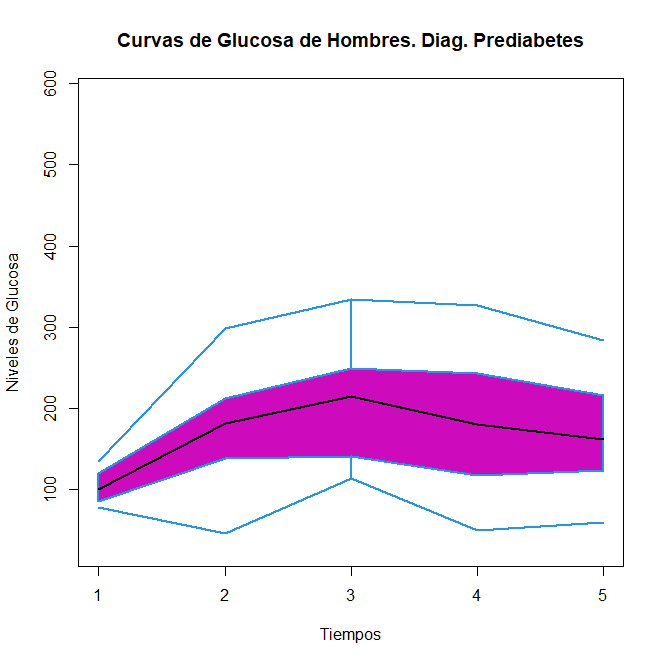
\includegraphics[width=0.45\textwidth]{img/bfHogluPredia.png}}
    \caption{Boxplot funcional para las curvas de glucosa para personas con prediagnóstico prediabetes.}
    \label{fig:glucosaPredia}
\end{figure}


En la Figura \ref{fig:insulinaPredia}, se muestran los boxplots funcionales de las curvas de insulina de ambos géneros en individuos prediabéticos. Uno de los aspectos más destacables son los outliers, que en ambos casos presentan valores muy altos. Este comportamiento podría ser indicativo de individuos con una resistencia a la insulina significativa, que están al borde de desarrollar diabetes.

\begin{figure}[H]
 \centering
  \subfloat[Mujeres]{
   \label{bfMuInsPredia}
    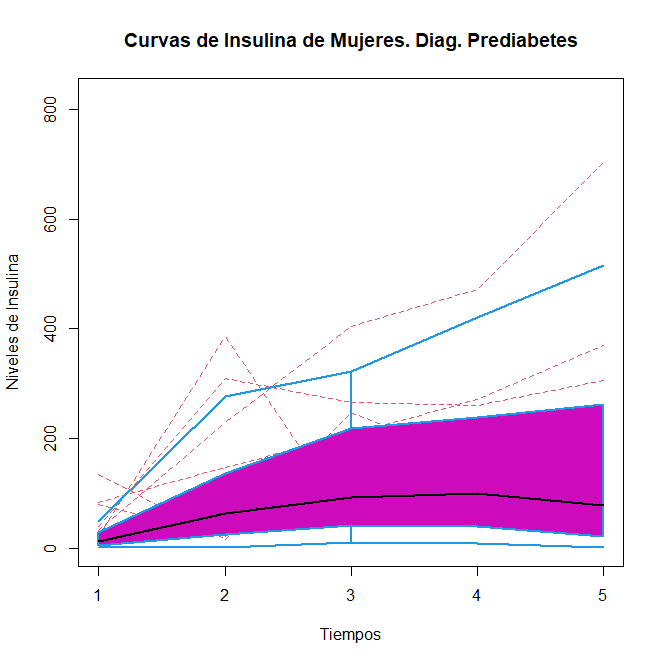
\includegraphics[width=0.45\textwidth]{img/bfMuInsPredia.png}}
  \subfloat[Hombres]{
   \label{bfHoInsPredia}
    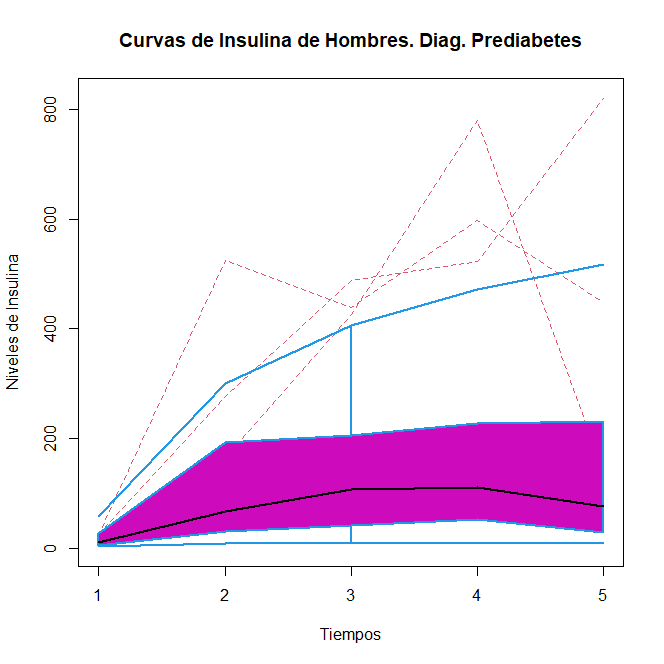
\includegraphics[width=0.45\textwidth]{img/bfHoInsPredia.png}}
    \caption{Boxplot funcional para las curvas de insulina para personas con prediagnóstico prediabetes.}
    \label{fig:insulinaPredia}
\end{figure}

En las mujeres, la curva mediana alcanza su máximo en el minuto 90, y el tercer cuartil se encuentra más separado de la mediana en comparación con el primer cuartil, lo que evidencia valores altos en los datos. Además, se aprecia una mayor varianza en los valores del minuto 120 en las mujeres en comparación con los hombres.


En los hombres, la curva mediana parece ser similar a la de las mujeres, pero los valores del tercer cuartil son ligeramente más bajos. Estos boxplots pueden resultar difíciles de discernir en cuanto a categorías, ya que la curva del primer cuartil es muy baja tanto en hombres como en mujeres, lo que podría indicar individuos con diabetes, y también se observan curvas muy altas.


%%%%%%%%%%%%%%%%%%%%%%%%%%%%%%%%%%%%%%%%%%%%%%%%%%

En la categoría diabética, en ambos boxplots funcionales las curvas medianas de glucosa se encuentran en un rango alto, alcanzando su máximo en el minuto $90$ para luego descender, ver Figura \ref{fig:glucosaDiabetes}. Sin embargo, en el caso de los hombres, la curva media desciende más rápidamente en comparación con las mujeres, donde parece ser más gradual. Es importante destacar que la varianza en el último instante es mayor en hombres, y se observa que el bigote superior alcanza niveles de alrededor de $600$.

\begin{figure}[H]
 \centering
  \subfloat[Mujeres]{
   \label{bfMuGluDia}
    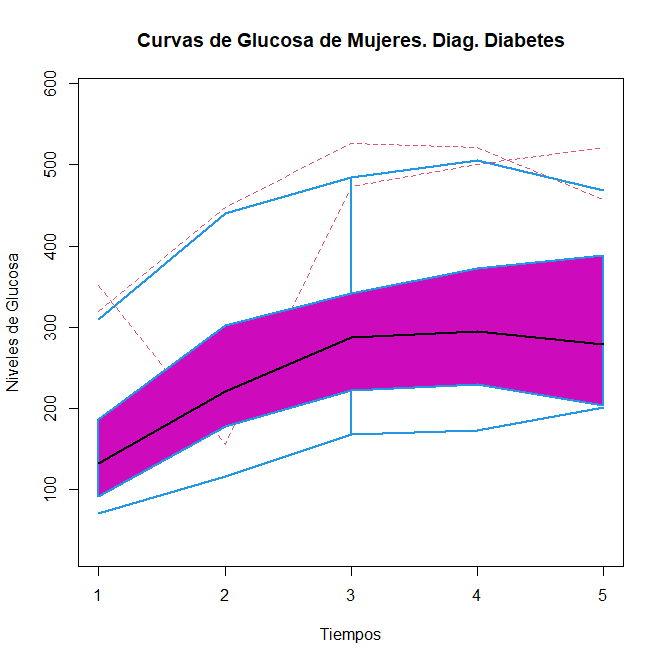
\includegraphics[width=0.45\textwidth]{img/bfMugluDiab.png}}
  \subfloat[Hombres]{
   \label{bfHoGluDia}
    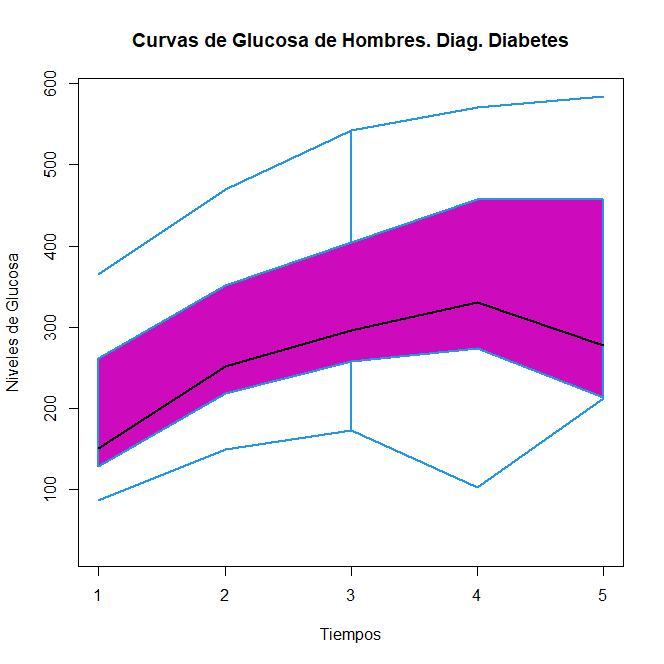
\includegraphics[width=0.45\textwidth]{img/bfHoGluDiabetes.png}}
    \caption{Boxplot funcional para las curvas de glucosa para personas con prediagnóstico diabetes.}
    \label{fig:glucosaDiabetes}
\end{figure}

Además, es notable que en esta categoría casi no hay outliers; en el boxplot de hombres no se presentan, y en el de mujeres hay dos, uno de los cuales muestra una caída muy abrupta en el minuto $30$, lo cual es biológicamente poco plausible y podría atribuirse a un error de medición. Similarmente, se observa una caída repentina en el bigote inferior de los hombres en el minuto $90$, lo que también podría ser atribuido a un error tipográfico.

En ambos casos parece haber un patrón discernible: en los hombres, el ascenso alcanza rangos más altos, mientras que en las mujeres parece ser un poco más suave. Sin embargo, sería difícil afirmar que esta diferencia es característica de cada género, ya que puede haber variabilidad individual significativa dentro de cada grupo.

\begin{figure}[H]
 \centering
  \subfloat[Mujeres]{
   \label{bfMuInsDia}
    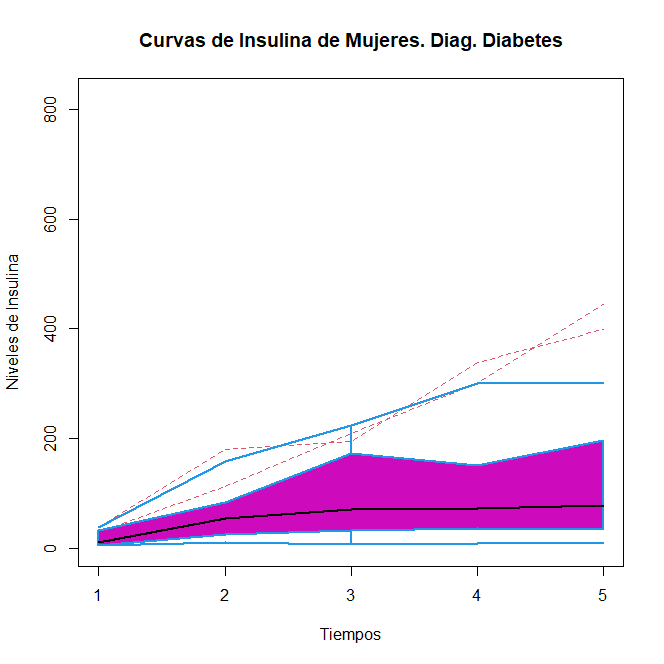
\includegraphics[width=0.45\textwidth]{img/bfMuInsDiabetes.png}}
  \subfloat[Hombres]{
   \label{bfHoInsDia}
    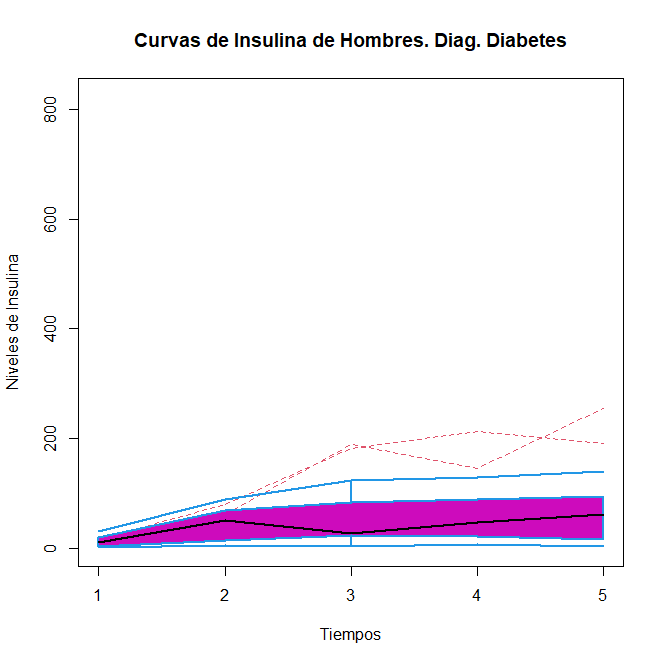
\includegraphics[width=0.45\textwidth]{img/bfHoInsDiabetes.png}}
    \caption{Boxplot funcional para las curvas de insulina para personas con prediagnóstico diabetes.}
    \label{fig:insulinaDiabetes}
\end{figure}

Los boxplots funcionales correspondientes a las curvas de insulina de la categoría diabética se muestran en la Figura \ref{fig:insulinaDiabetes}. Estos boxplots parecen presentar características significativas. La curva mediana correspondiente al grupo de hombres es más baja que la de mujeres. Por otro lado, las curvas asociadas al primer y tercer cuartil de la categoría de hombres están muy cercanas a la mediana, lo que indica poca variabilidad. En cambio, las curvas del primer y tercer cuartil de mujeres están más separadas, lo que indica mayor variabilidad.

Varias curvas representativas de ambos boxplots muestran el comportamiento inusual de subir, bajar y luego volver a subir. Aunque estos cambios pueden atribuirse a errores de medición, dado que no son extremadamente abruptos, no se descartarán. Los outliers son de escala, sin embargo, siguen este patrón de solo ascenso y en cantidades reducidas, lo cual concuerda con el perfil diabético.

\begin{landscape}
\subsection{Visualización del Modelo ajustado para Mujeres}

\begin{figure}[H]
    \centering
    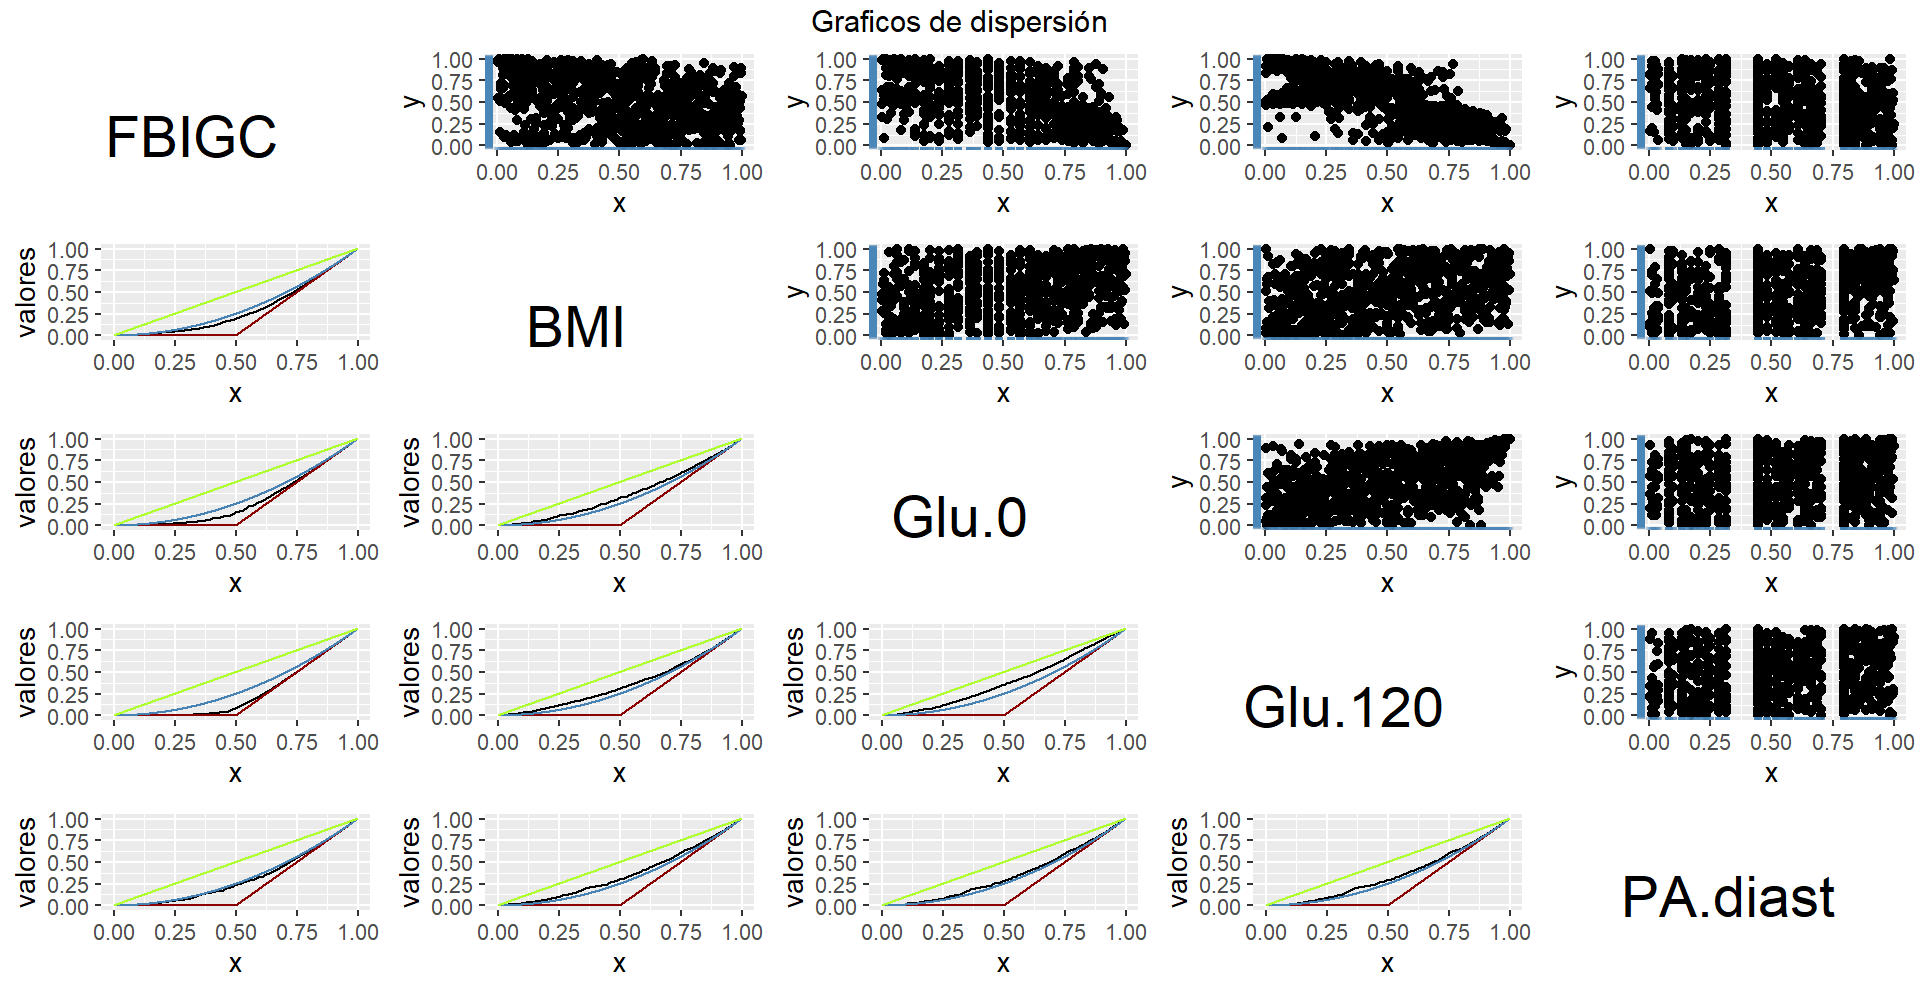
\includegraphics[height = 13.5 cm, width = 1.4 \textwidth]{4img/UdiagM.png}
    \caption{Diagonales y gráficos de dispersión en escala $u$.}
    \label{fig:diagMU}
\end{figure}
\end{landscape}

\begin{figure}[H]
 \centering
  \subfloat[$\mathscr{H}\rho_{C_{12}}$]{
   \label{C12rho}
    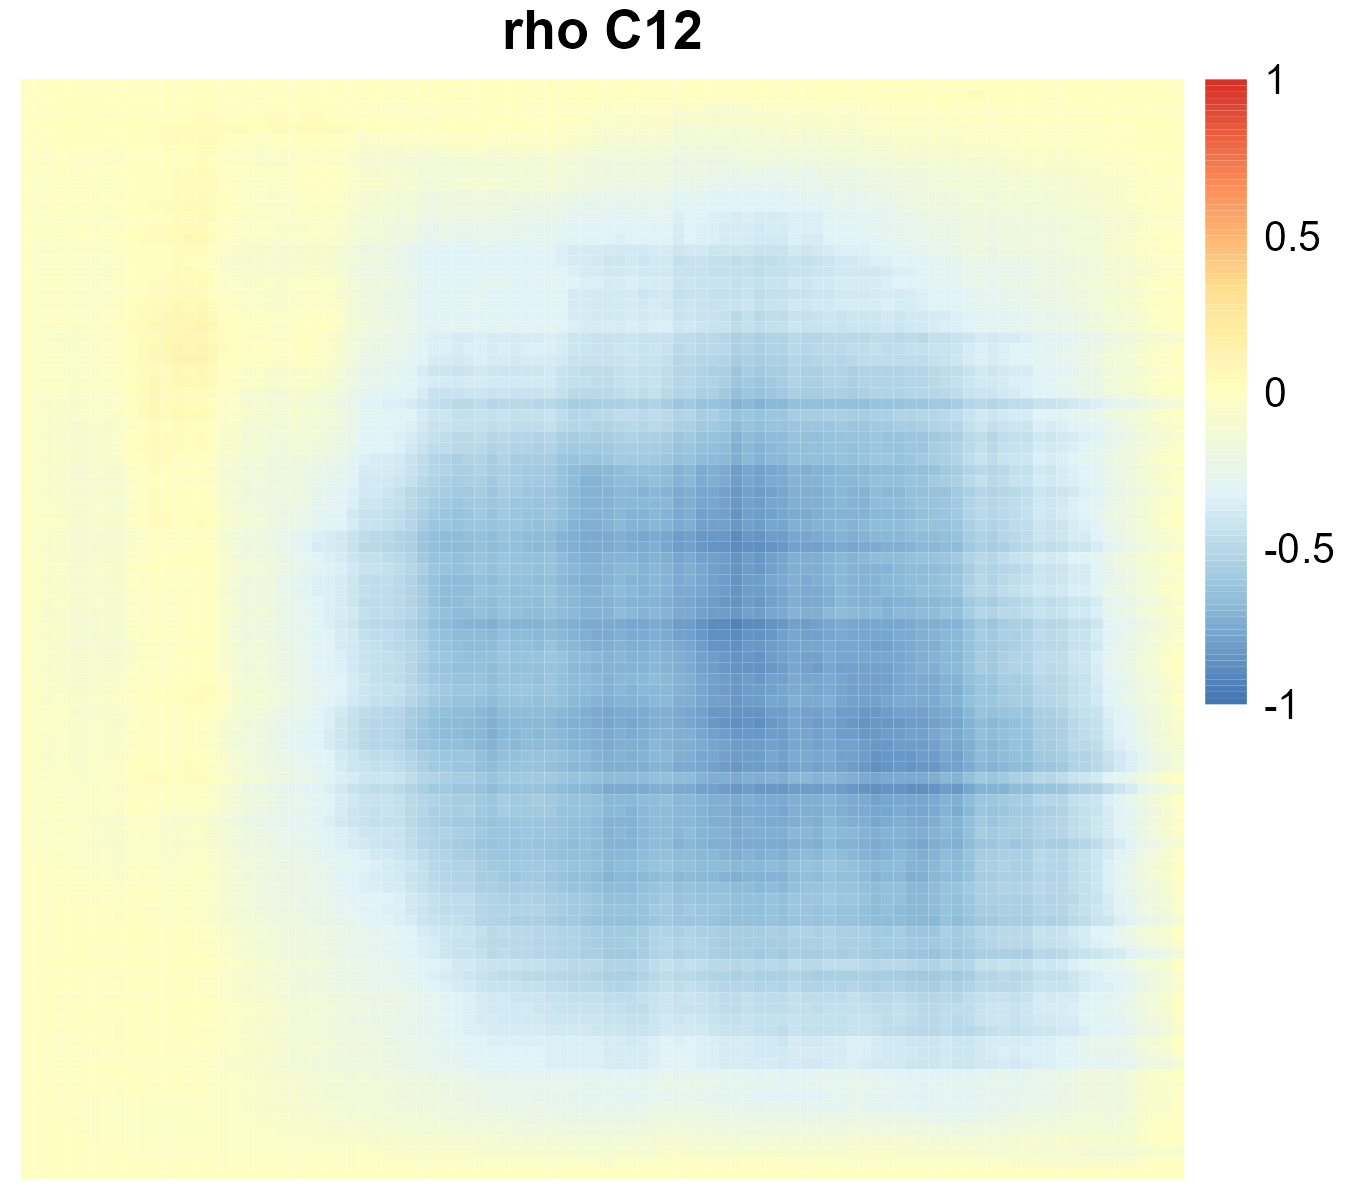
\includegraphics[width=0.33\textwidth]{4img/MujrhoC12.png}}
  \subfloat[$\mathscr{H}\sigma_{C_{12}}$]{
   \label{C12sigma}
    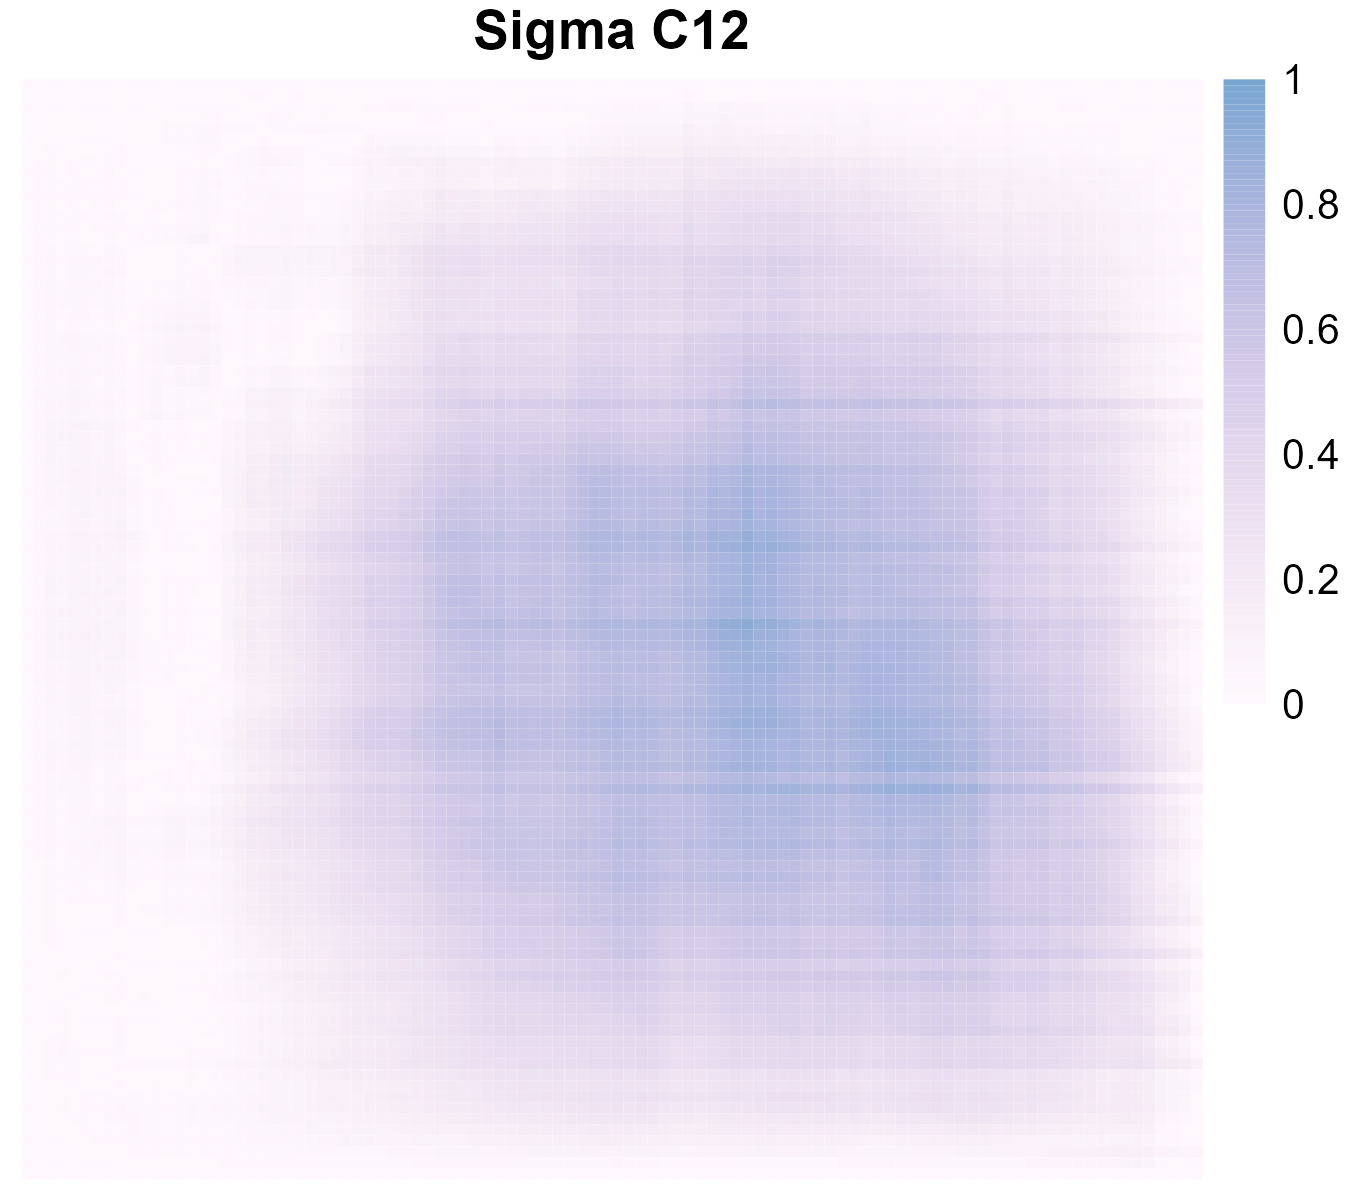
\includegraphics[width=0.33\textwidth]{4img/MujsigmaC12.png}}
  \subfloat[$\mathscr{H}_{C_{12}}$]{
   \label{C12H}
    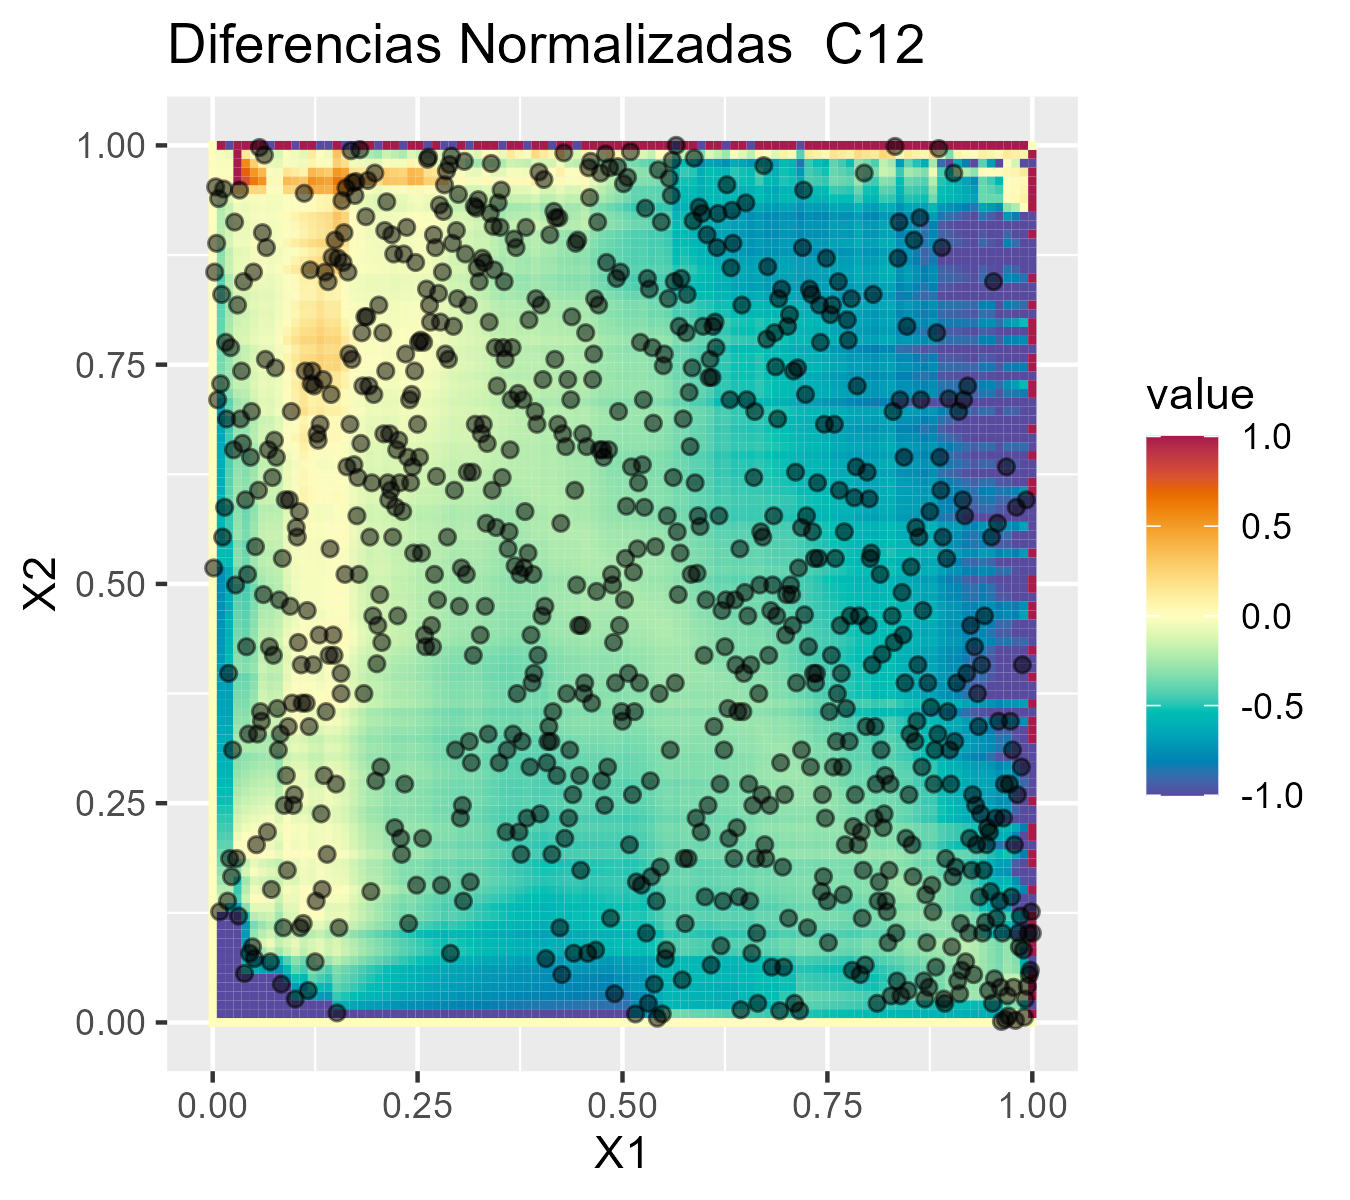
\includegraphics[width=0.33\textwidth]{4img/MujHC12.png}}
\end{figure}

\begin{figure}[H]
 \centering
  \subfloat[$\mathscr{H}\rho_{C_{23}}$]{
   \label{C23rho}
    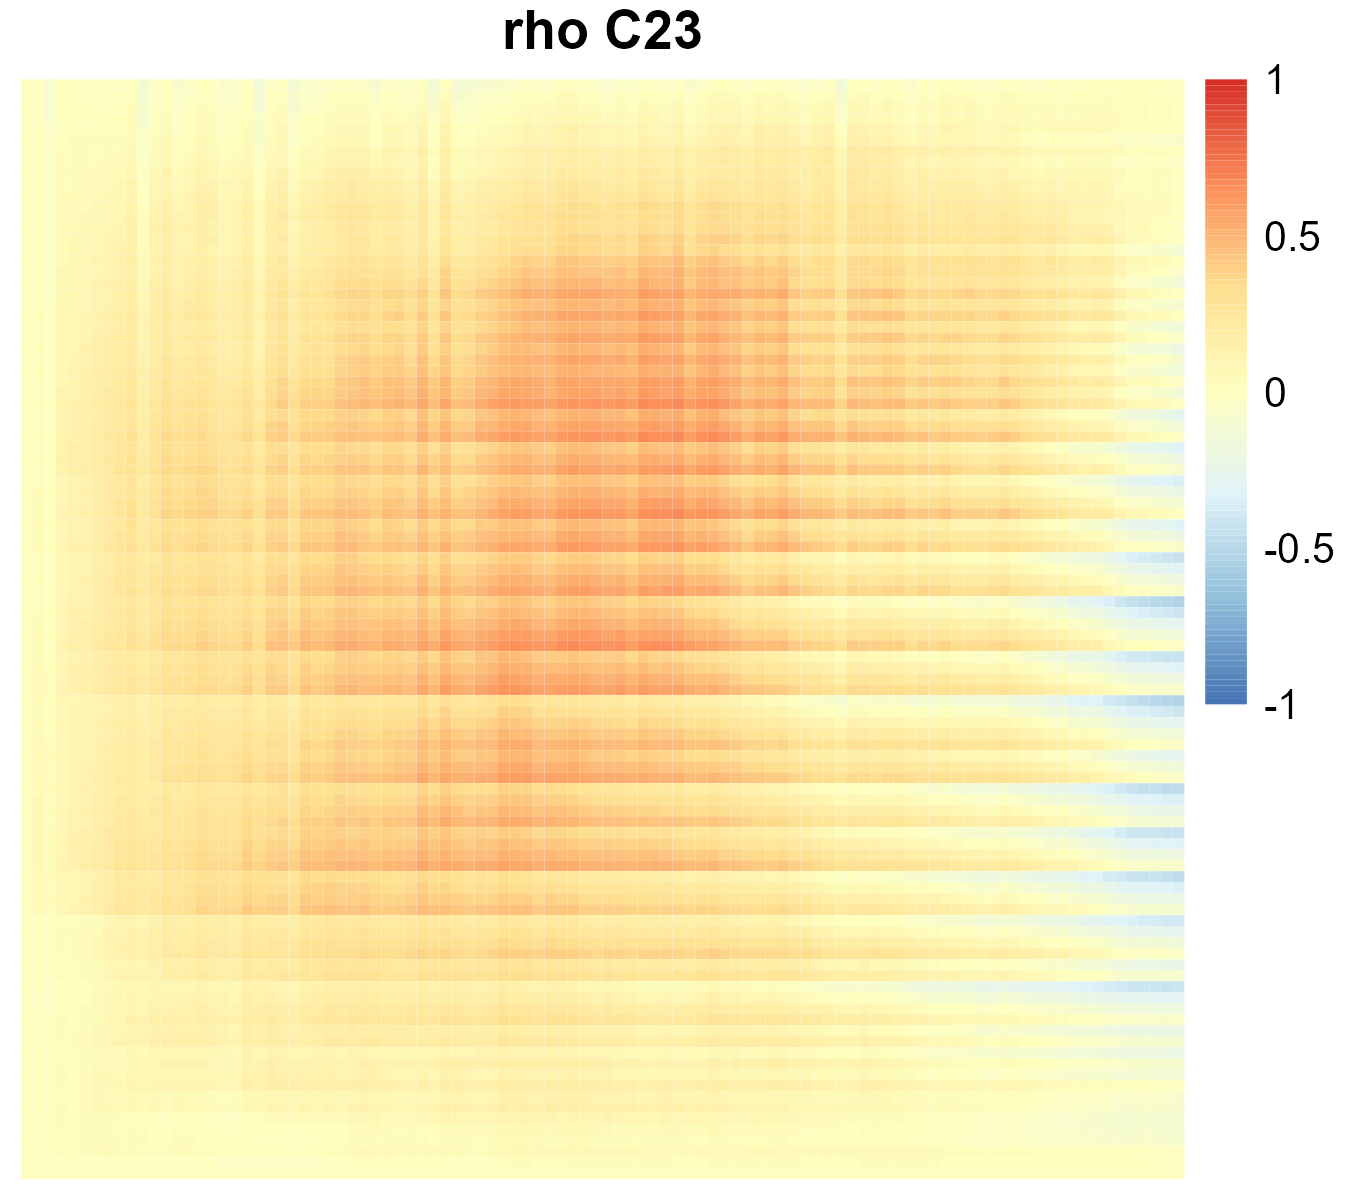
\includegraphics[width=0.33\textwidth]{4img/MujrhoC23.png}}
  \subfloat[$\mathscr{H}\sigma_{C_{23}}$]{
   \label{C23sigma}
    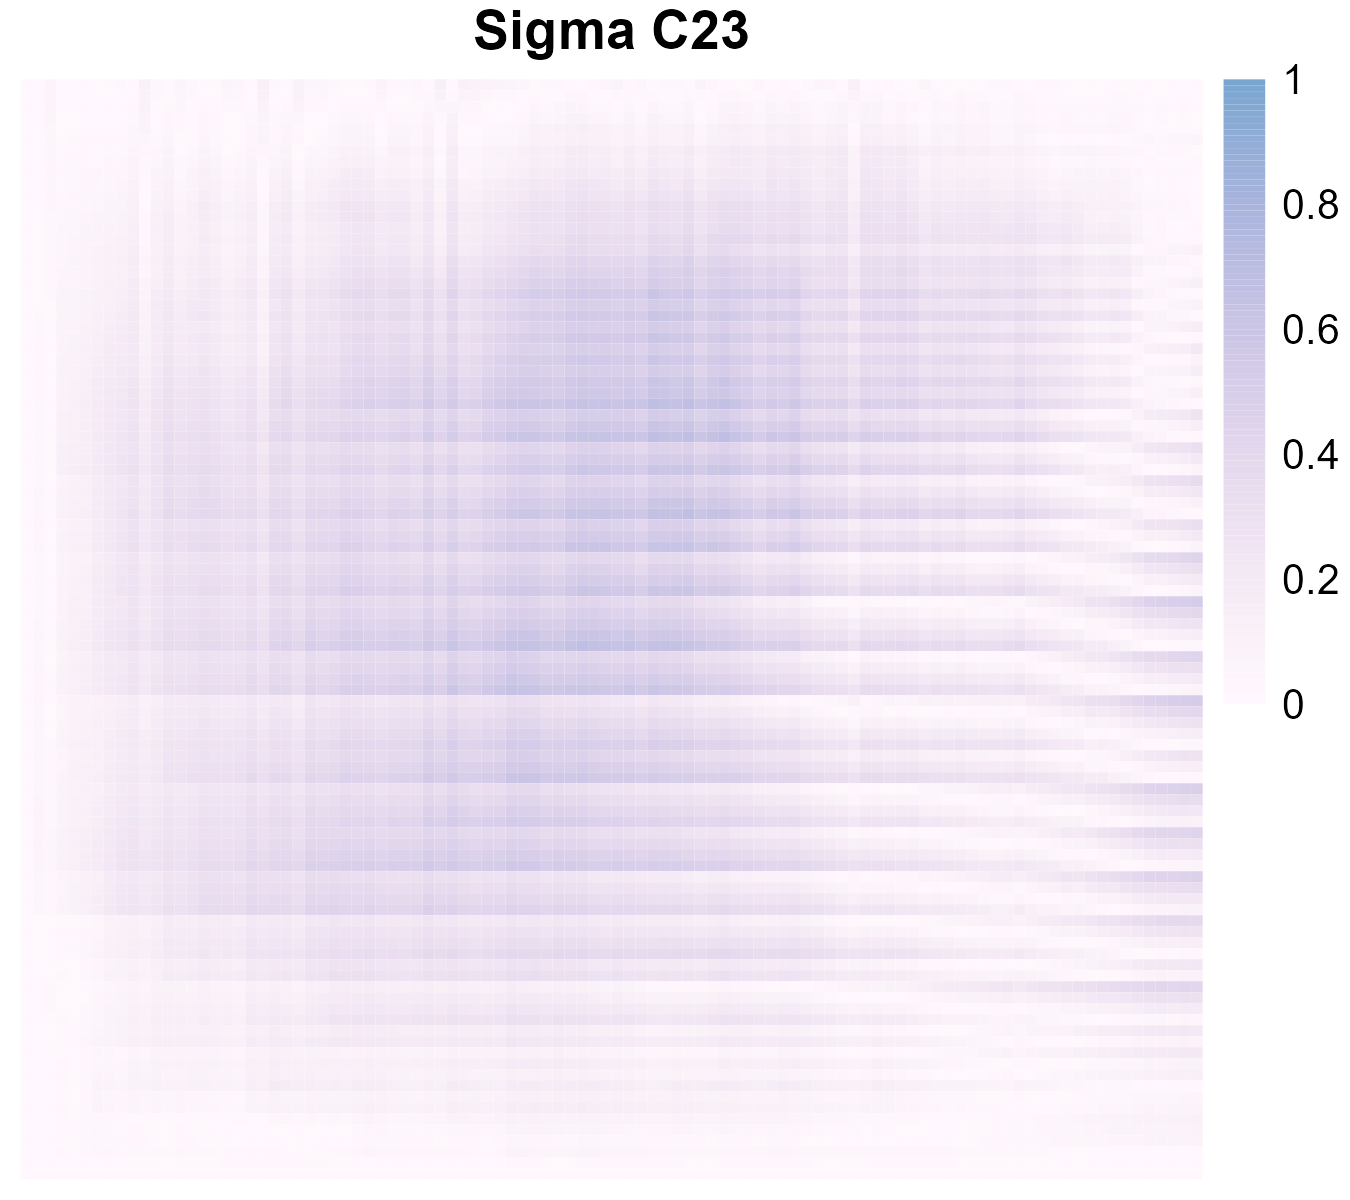
\includegraphics[width=0.33\textwidth]{4img/MujsigmaC23.png}}
  \subfloat[$\mathscr{H}_{C_{23}}$]{
   \label{C23H}
    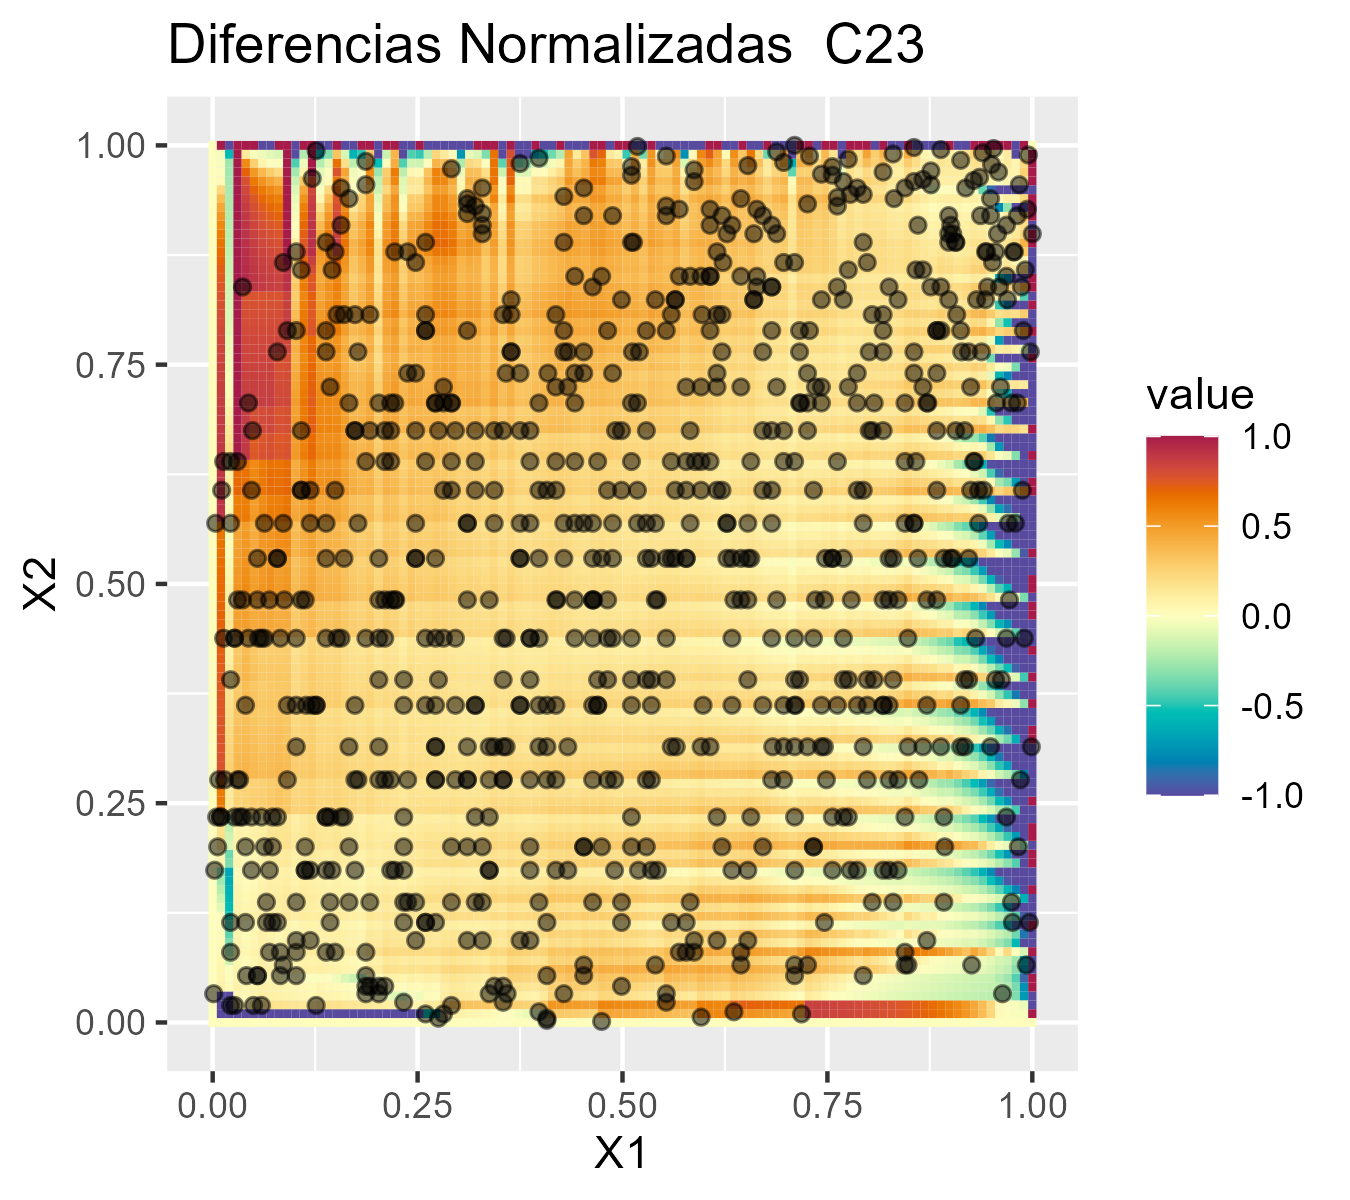
\includegraphics[width=0.33\textwidth]{4img/MujHC23.png}}
\end{figure}

\begin{figure}[H]
 \centering
  \subfloat[$\mathscr{H}\rho_{C_{34}}$]{
   \label{C34rho}
    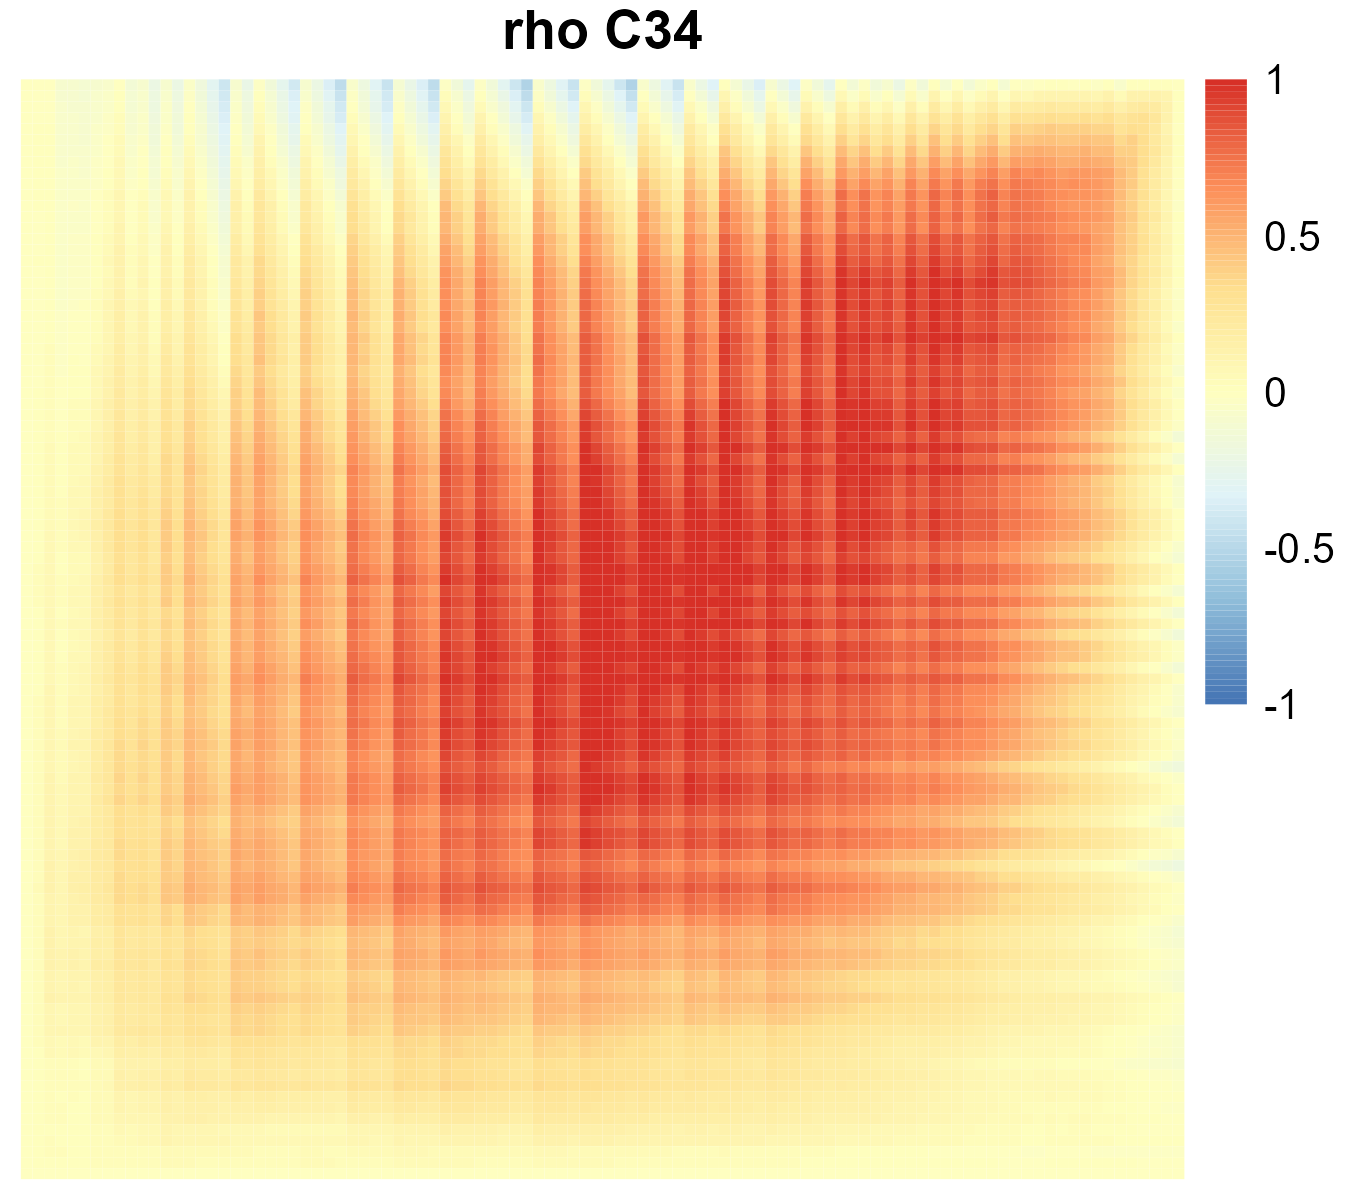
\includegraphics[width=0.33\textwidth]{4img/MujrhoC34.png}}
  \subfloat[$\mathscr{H}\sigma_{C_{34}}$]{
   \label{C34sigma}
    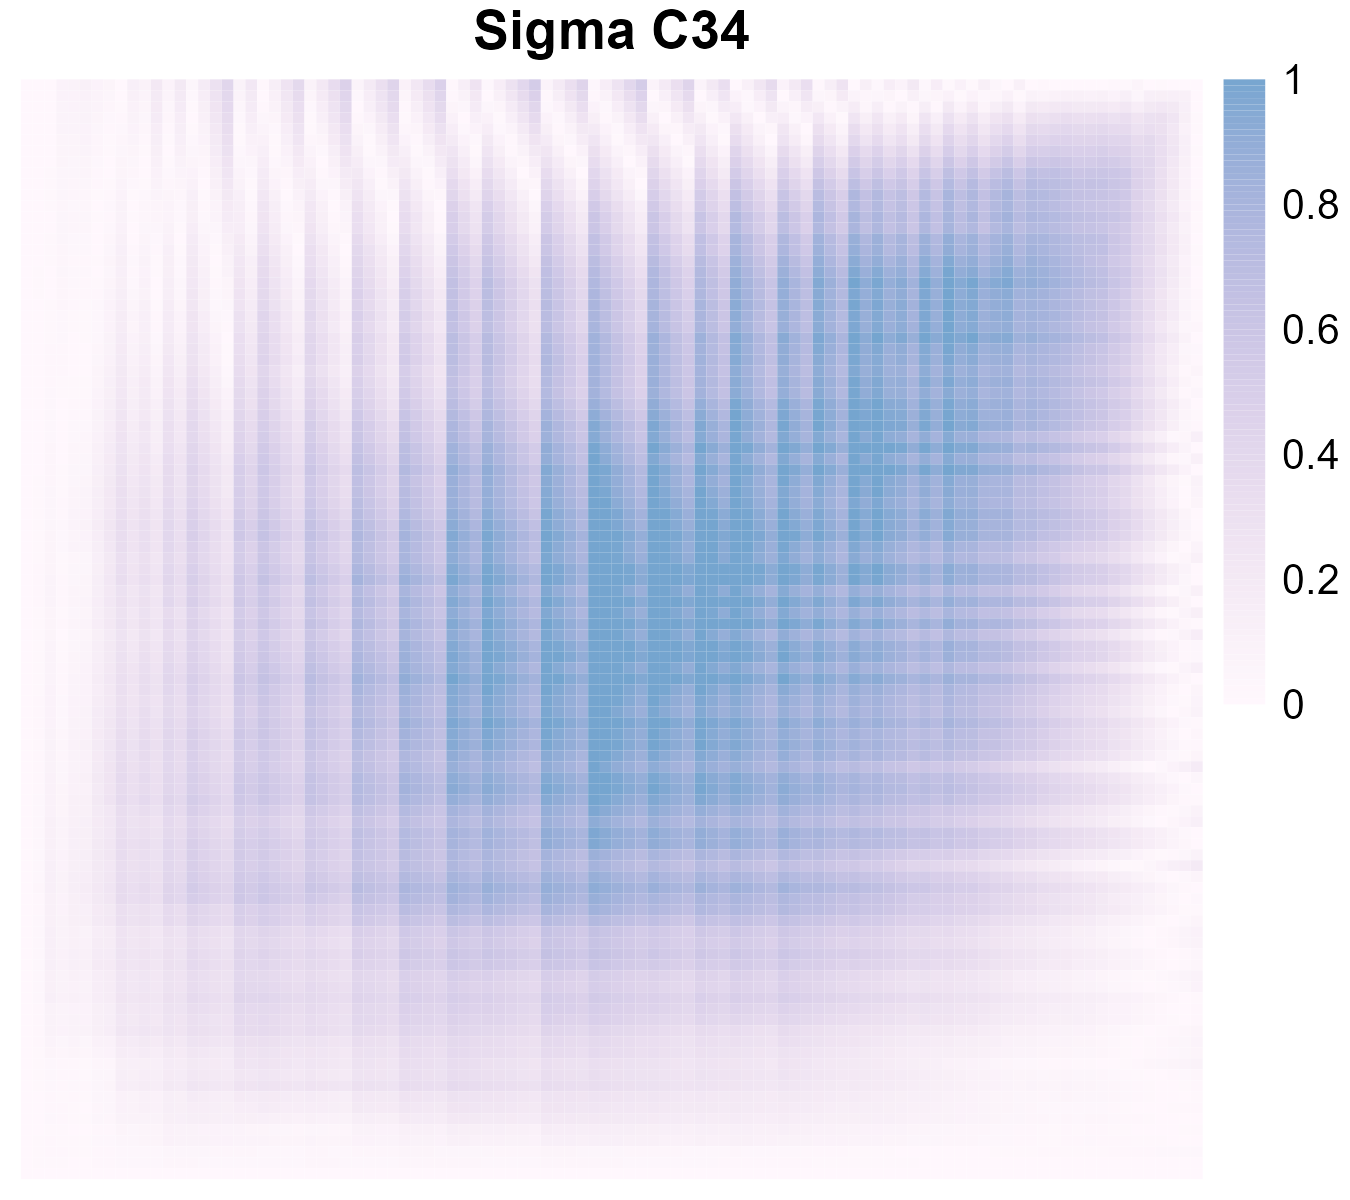
\includegraphics[width=0.33\textwidth]{4img/MujsigmaC34.png}}
  \subfloat[$\mathscr{H}_{C_{34}}$]{
   \label{C34H}
    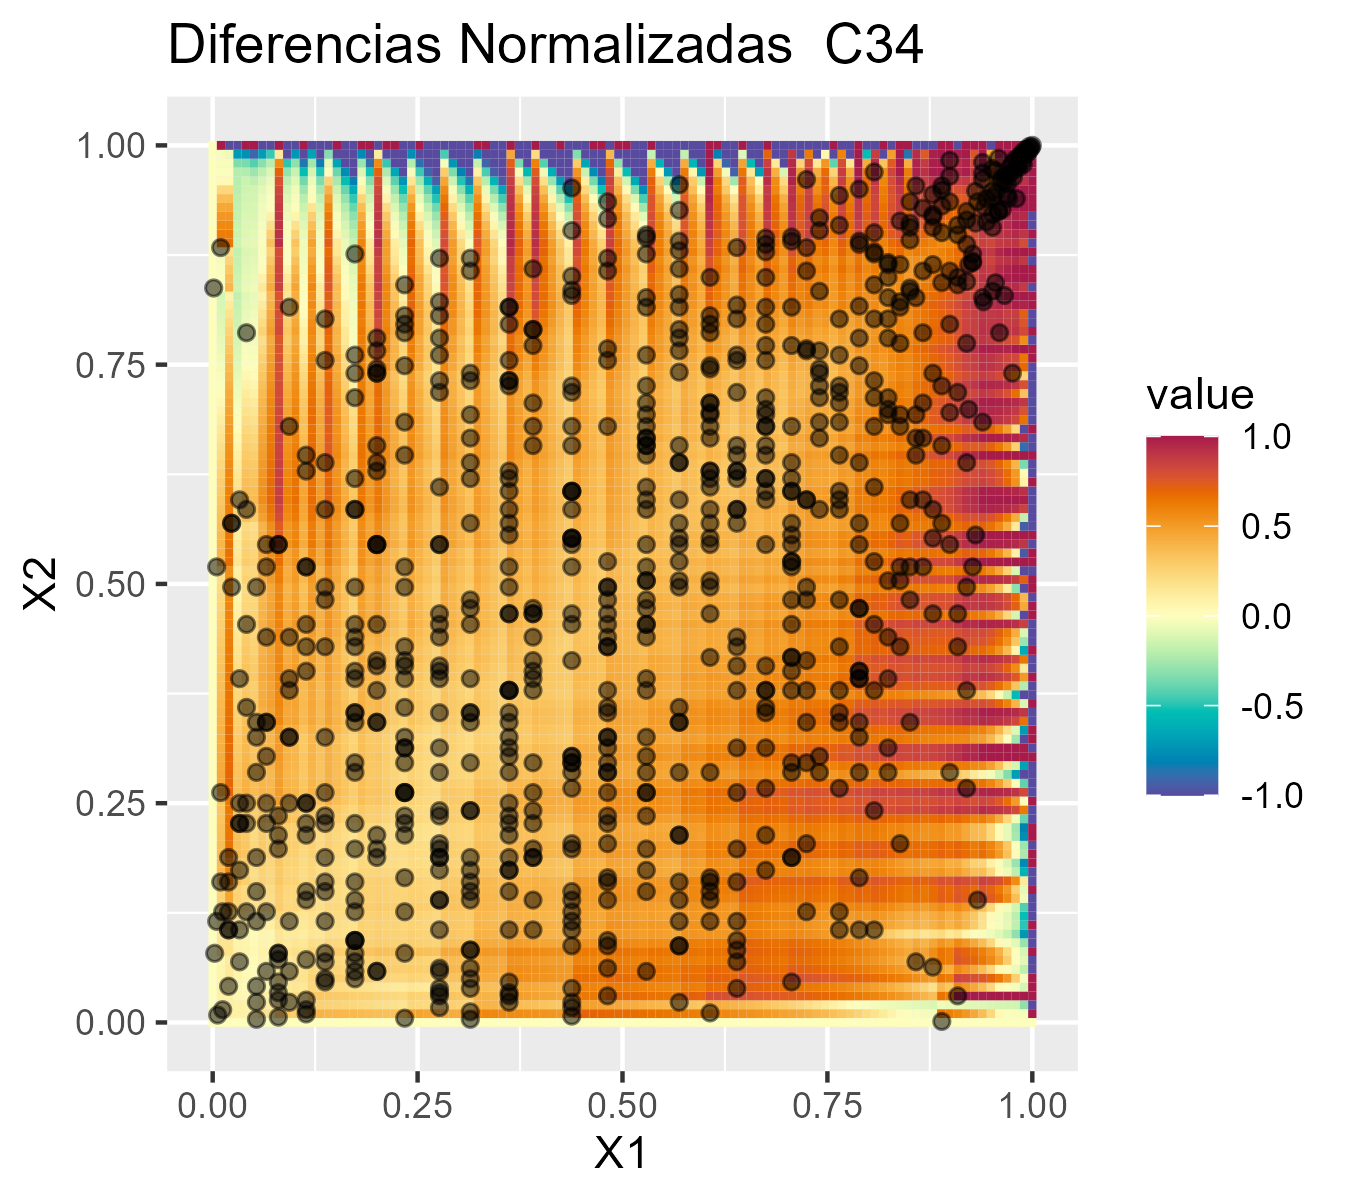
\includegraphics[width=0.33\textwidth]{4img/MujHC34.png}}
\end{figure}

\begin{figure}[H]
 \centering
  \subfloat[$\mathscr{H}\rho_{C_{45}}$]{
   \label{C45rho}
    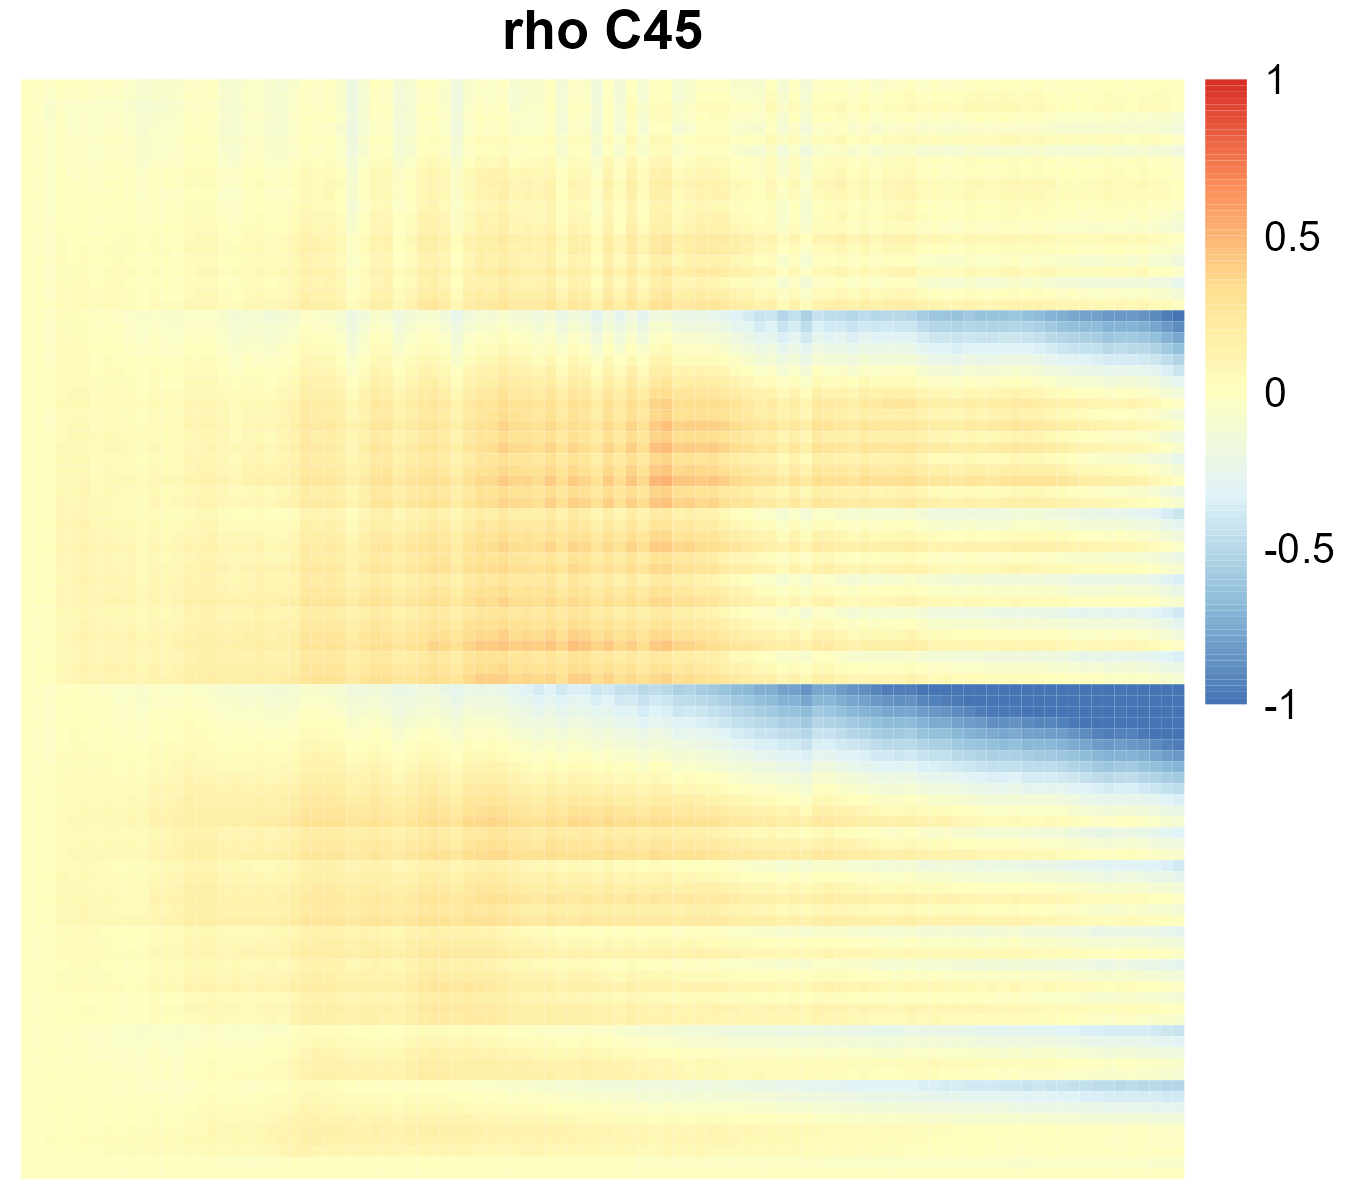
\includegraphics[width=0.33\textwidth]{4img/MujrhoC45.png}}
  \subfloat[$\mathscr{H}\sigma_{C_{45}}$]{
   \label{C45sigma}
    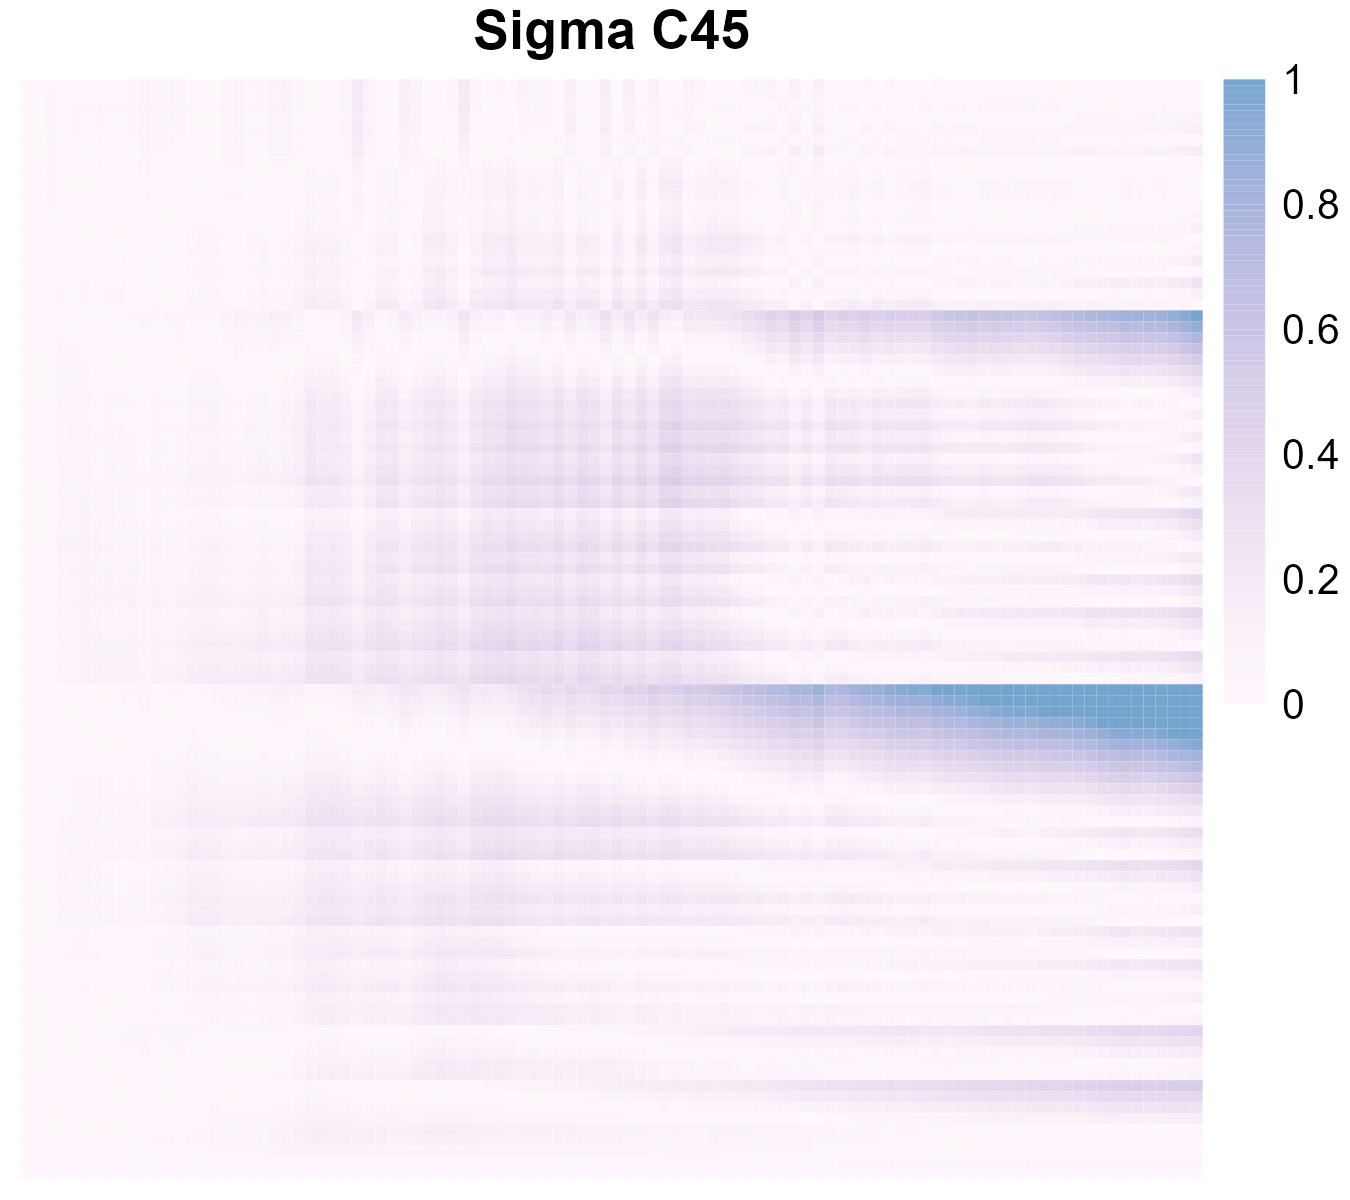
\includegraphics[width=0.33\textwidth]{4img/MujsigmaC45.png}}
  \subfloat[$\mathscr{H}_{C_{45}}$]{
   \label{C45H}
    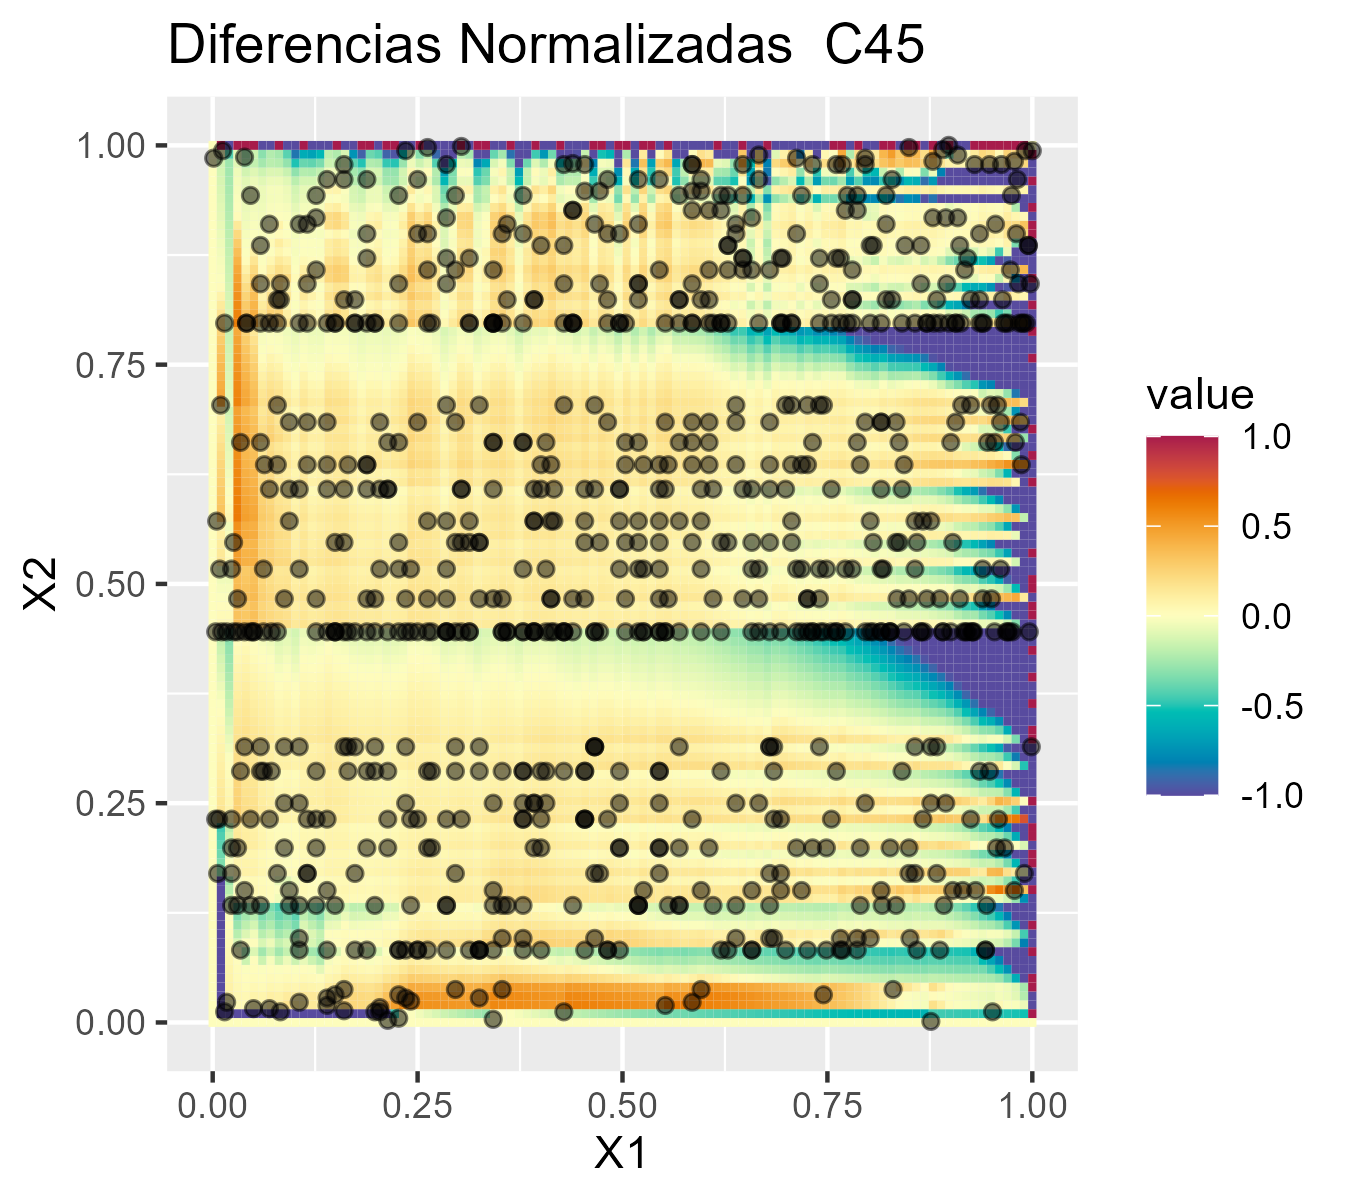
\includegraphics[width=0.33\textwidth]{4img/MujHC45.png}}
    \caption{Cópulas Ajustadas para Mujeres, nivel $1$.}
    \label{fig:Modelo4MujNivel1}
\end{figure}

%%%%%%%%%%%%%%%%%%%%%%%%%%%%%%%%%%%%%%%%%%%%%%%%%%

\begin{figure}[H]
 \centering
  \subfloat[$\mathscr{H}\rho_{C_{13|2}}$]{
   \label{C13.2rho}
    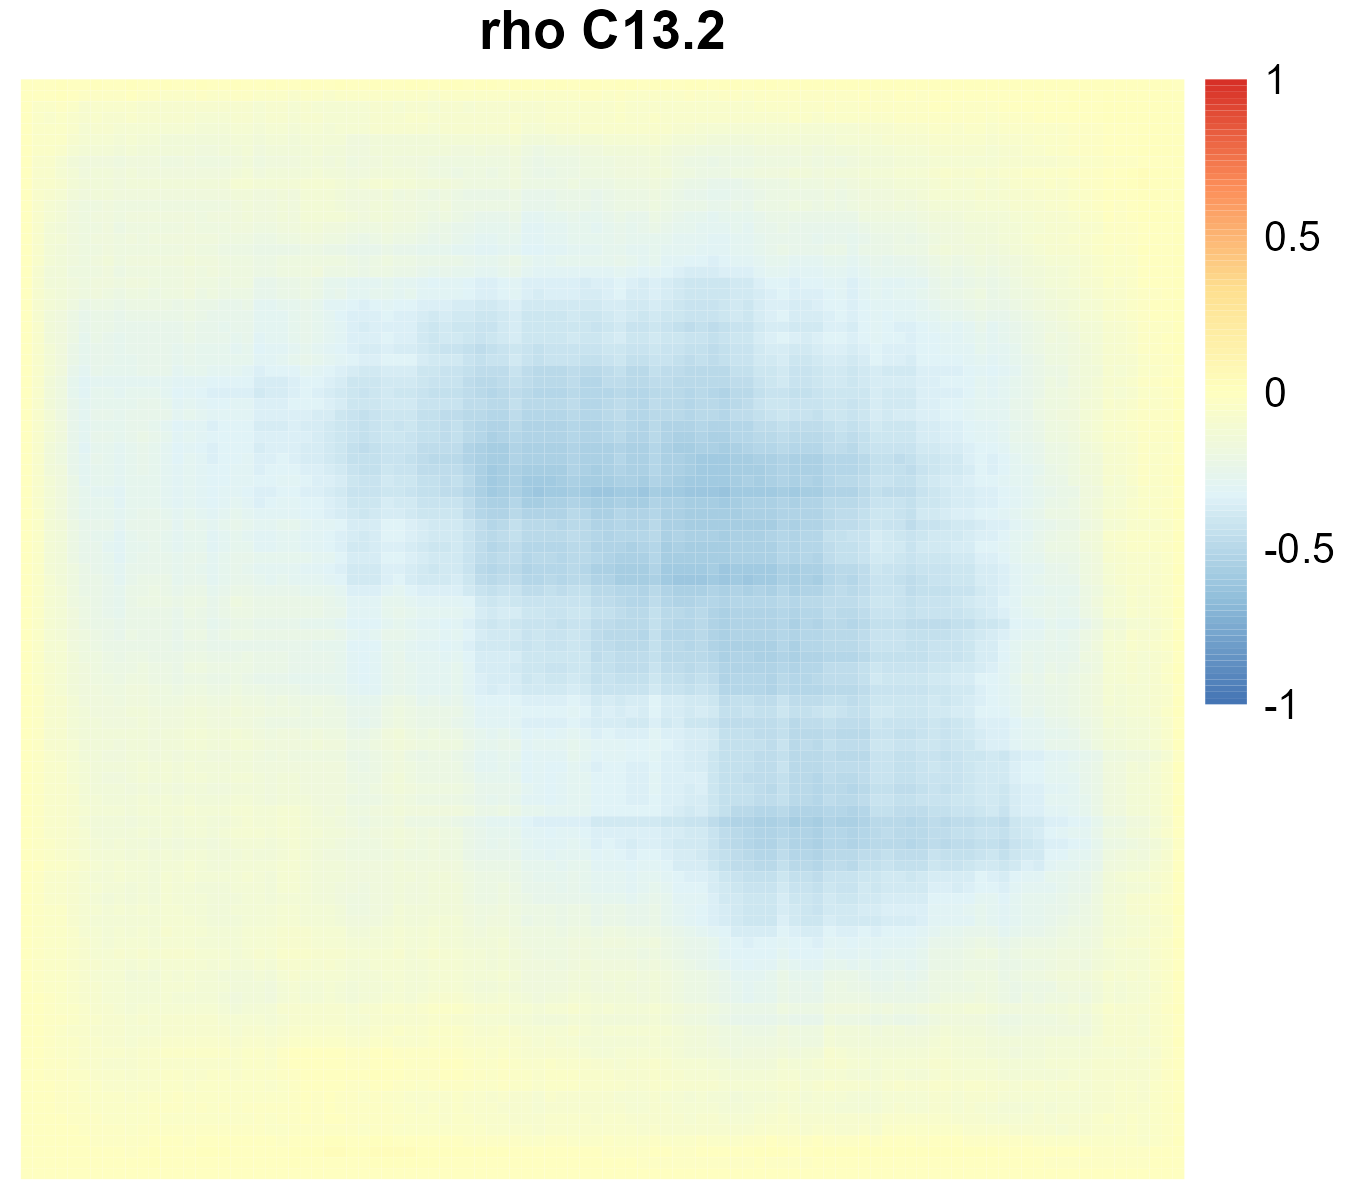
\includegraphics[width=0.33\textwidth]{4img/MujrhoC13.2.png}}
  \subfloat[$\mathscr{H}\sigma_{C_{13|2}}$]{
   \label{C13.2sigma}
    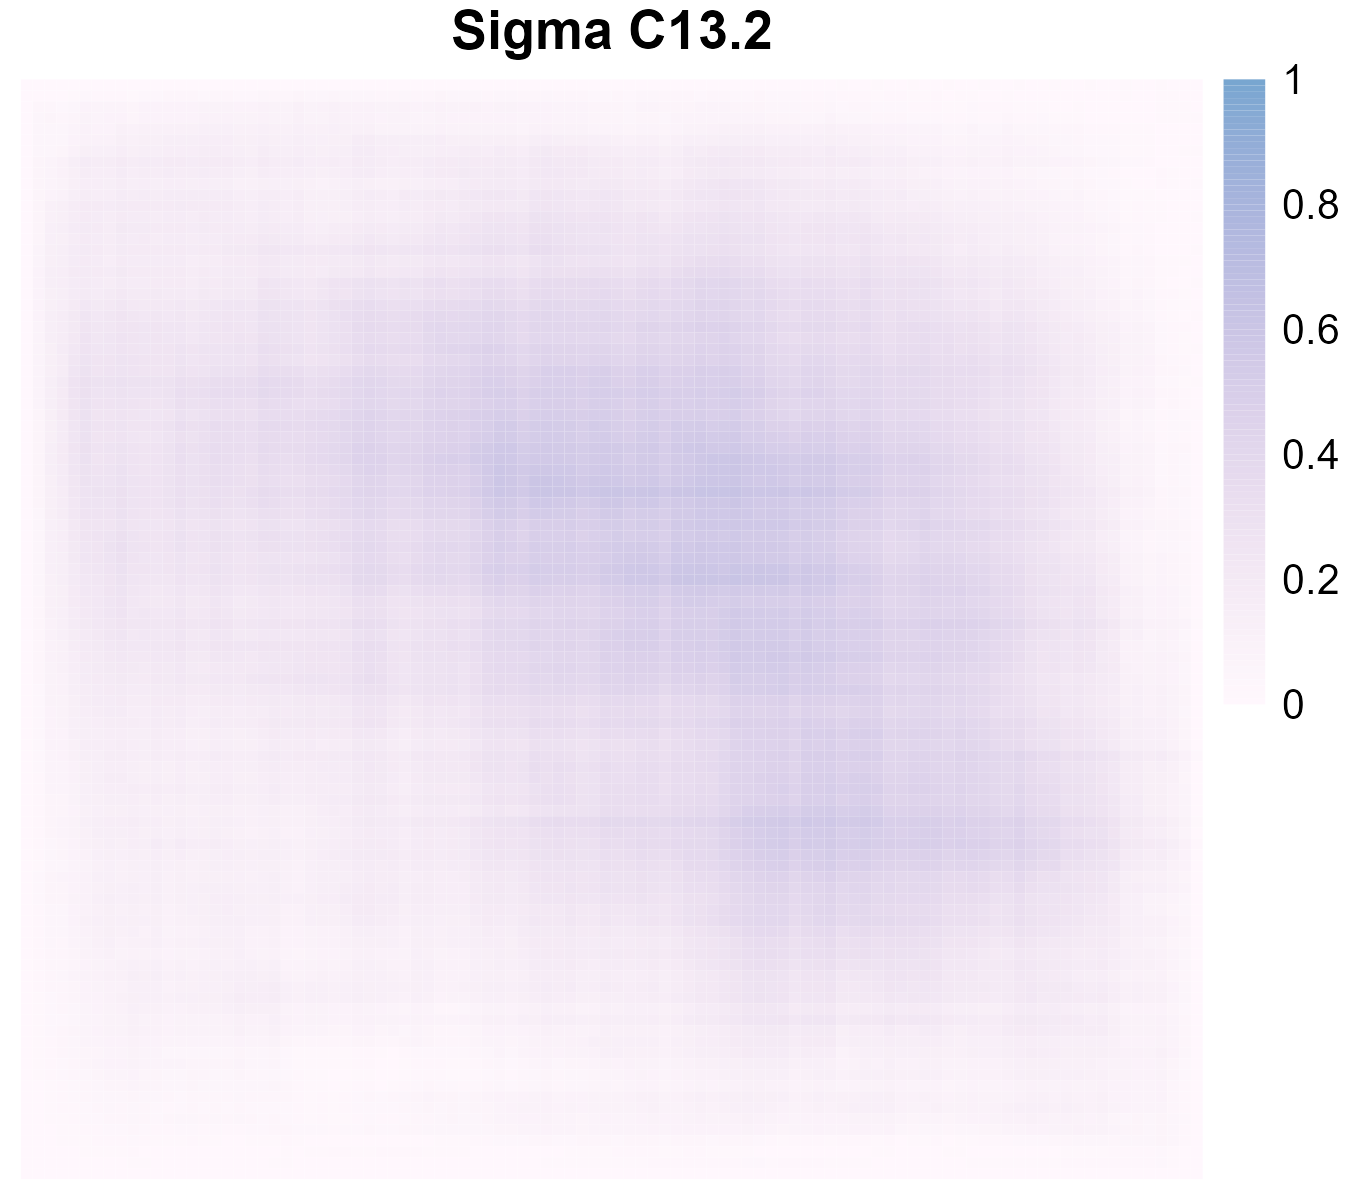
\includegraphics[width=0.33\textwidth]{4img/MujsigmaC13.2.png}}
  \subfloat[$\mathscr{H}_{C_{13|2}}$]{
   \label{C13.2H}
    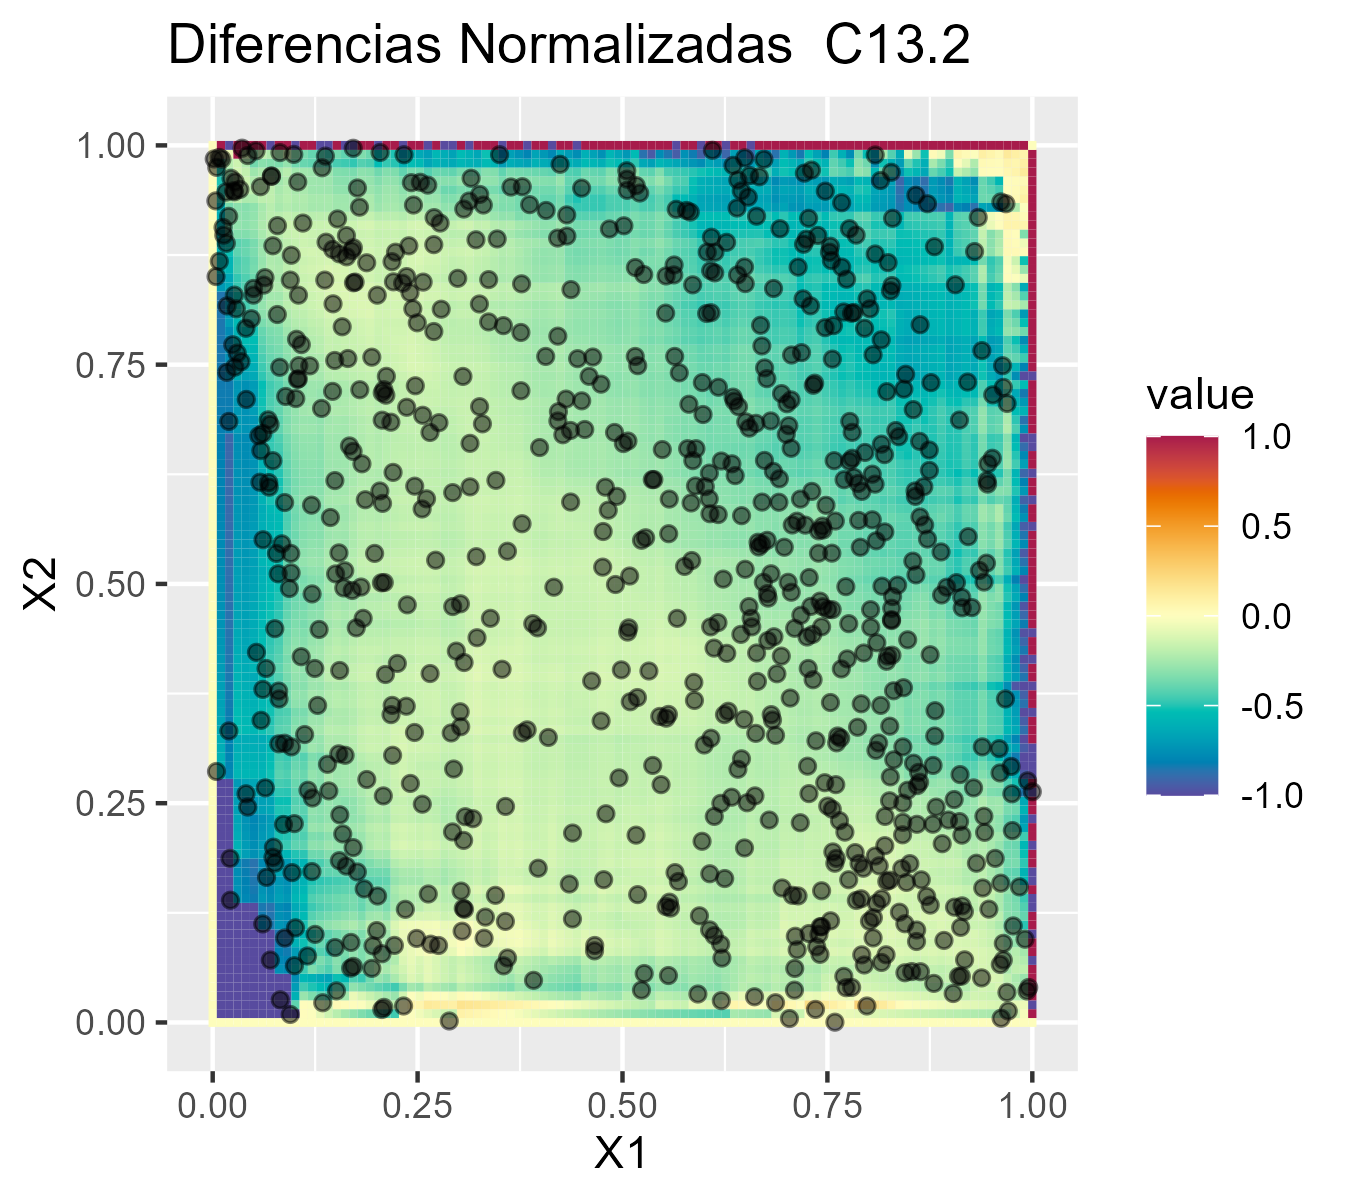
\includegraphics[width=0.33\textwidth]{4img/MujHC13.2.png}}
\end{figure}

\begin{figure}[H]
 \centering
  \subfloat[$\mathscr{H}\rho_{C_{24|3}}$]{
   \label{C24.3rho}
    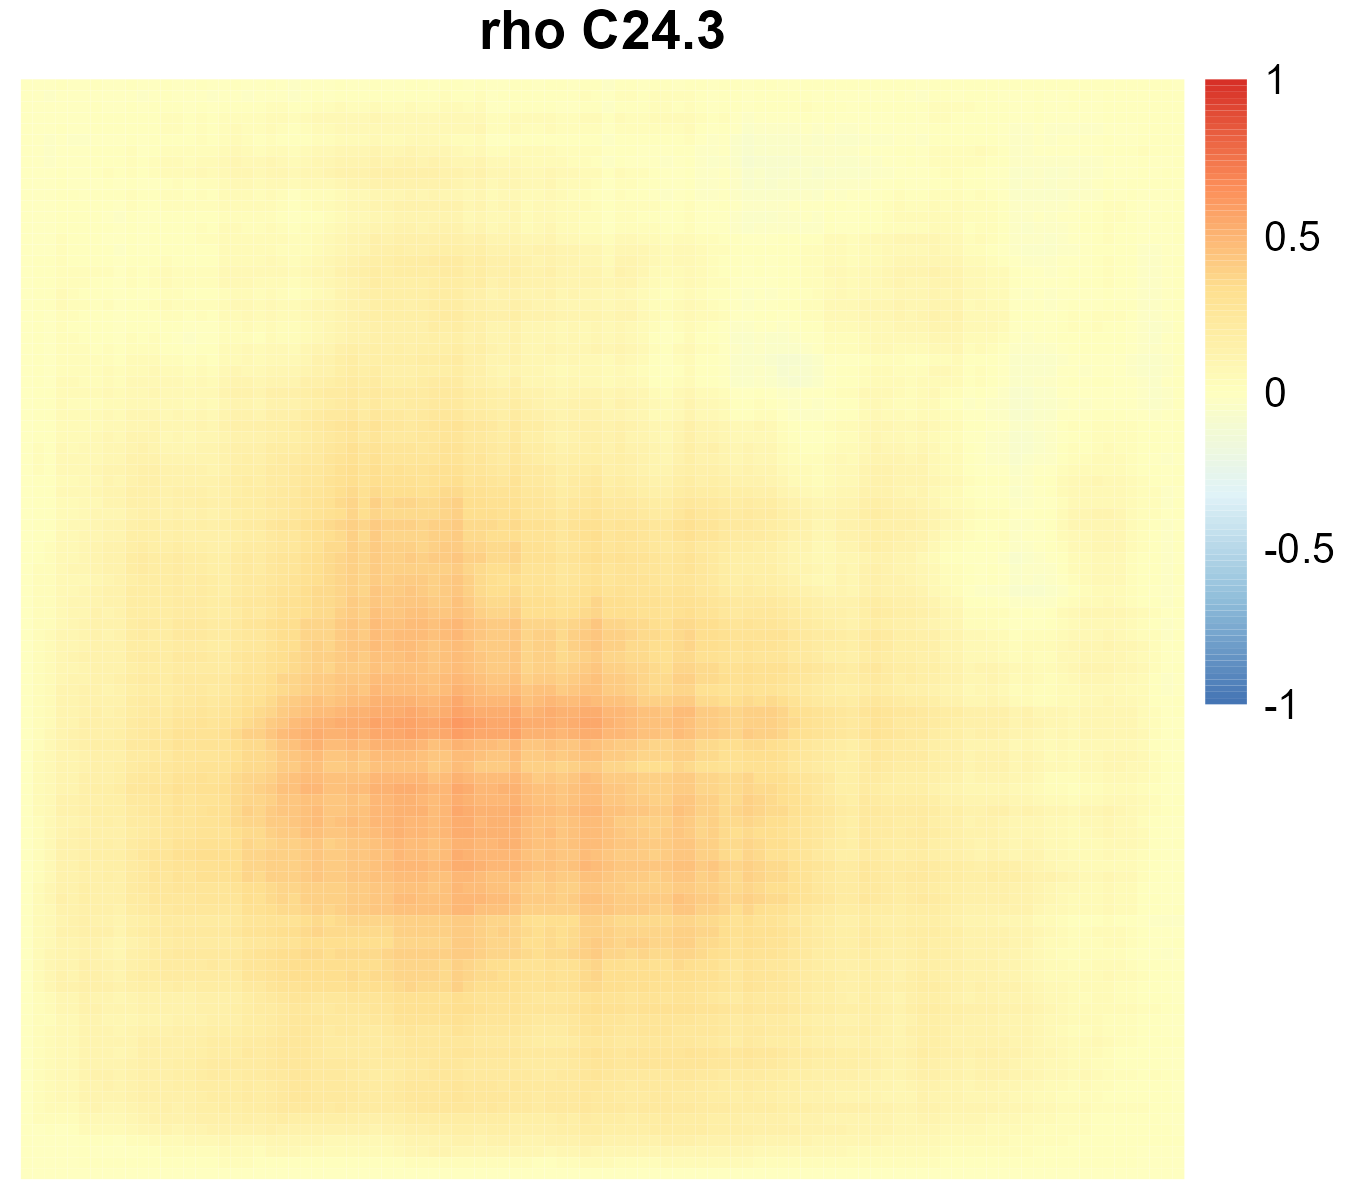
\includegraphics[width=0.33\textwidth]{4img/MujrhoC24.3.png}}
  \subfloat[$\mathscr{H}\sigma_{C_{24|3}}$]{
   \label{C24.3sigma}
    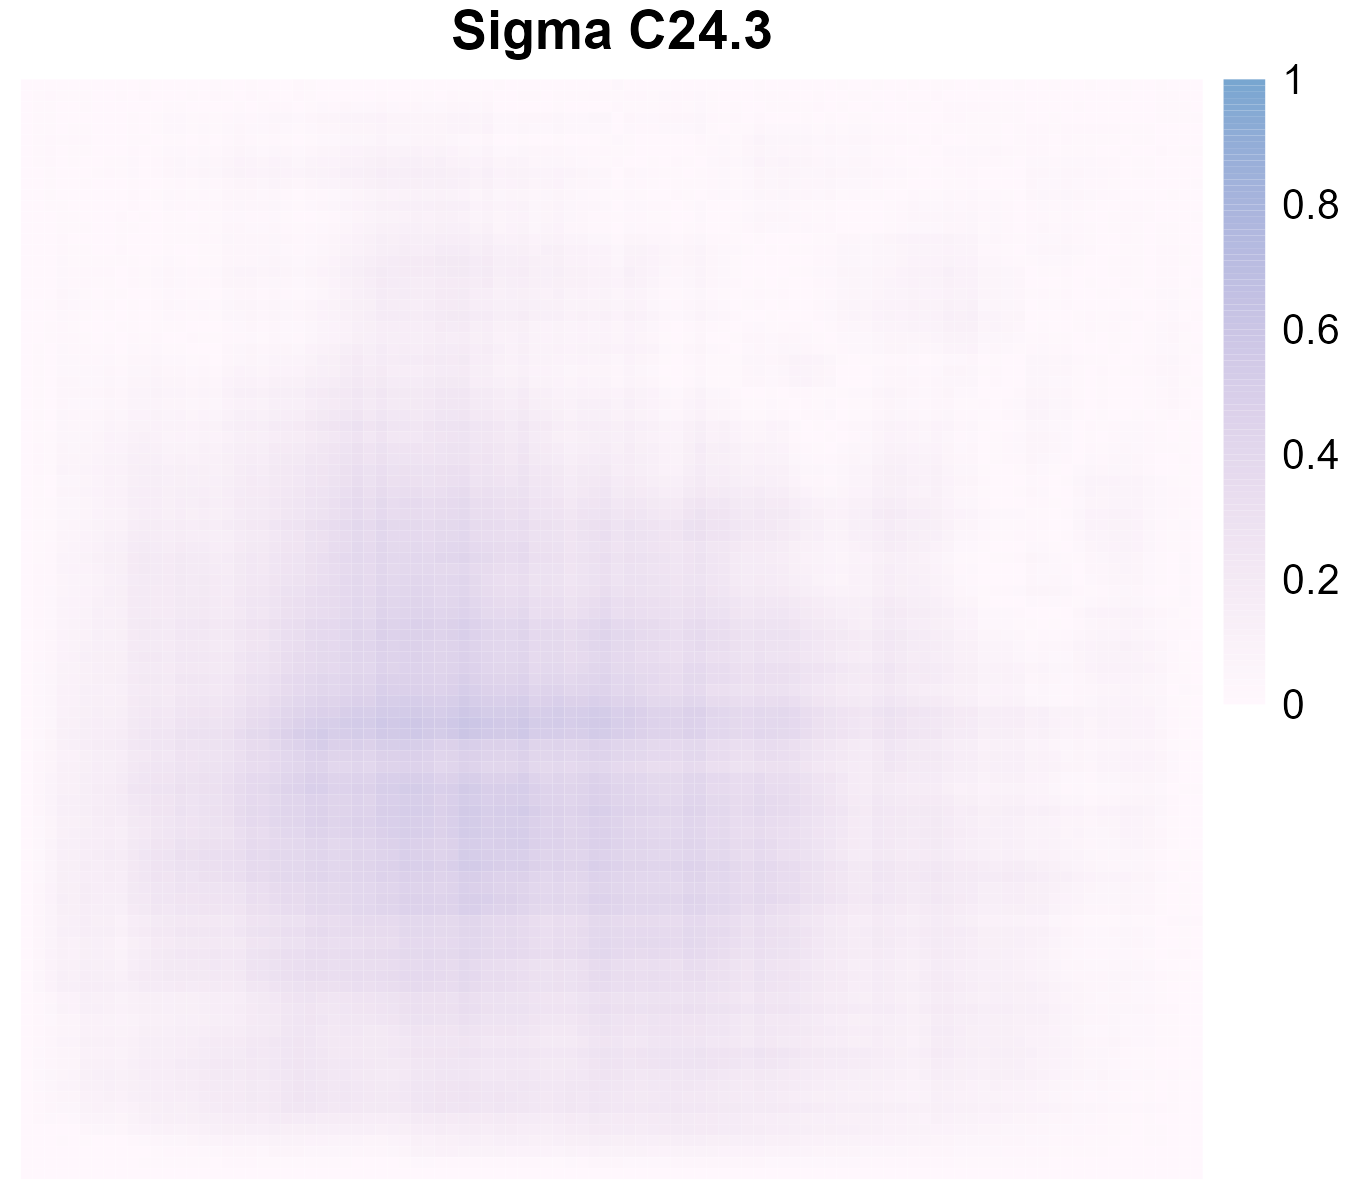
\includegraphics[width=0.33\textwidth]{4img/MujsigmaC24.3.png}}
  \subfloat[$\mathscr{H}_{C_{24|3}}$]{
   \label{C24.3H}
    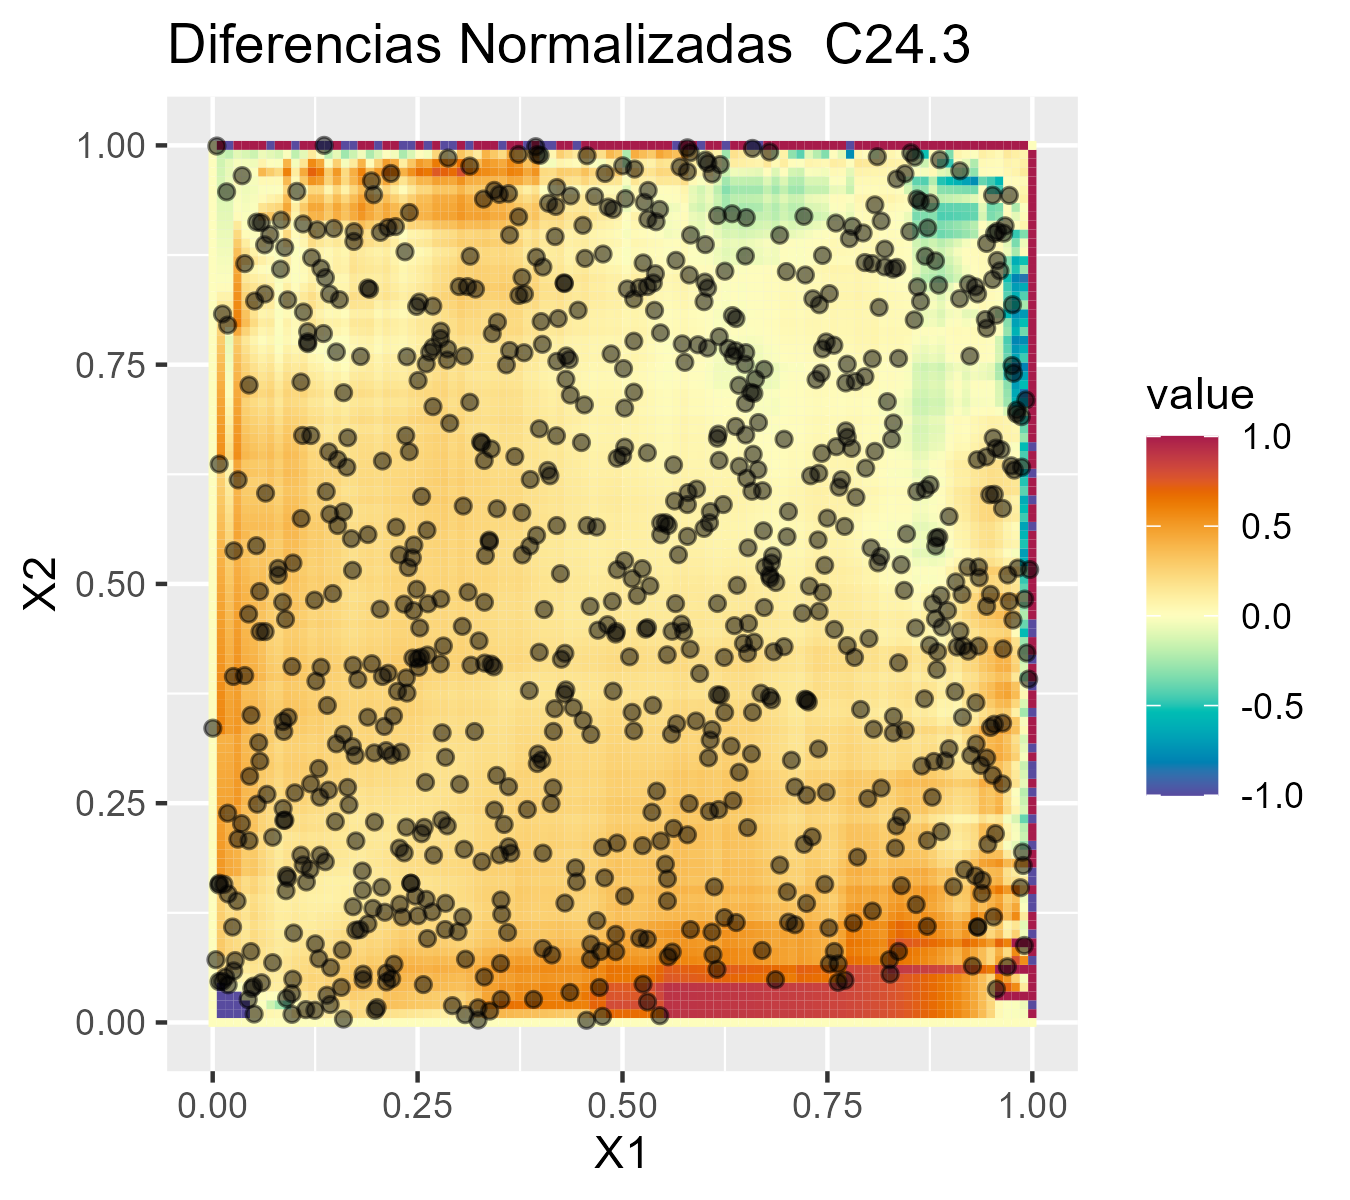
\includegraphics[width=0.33\textwidth]{4img/MujHC24.3.png}}
\end{figure}

\begin{figure}[H]
 \centering
  \subfloat[$\mathscr{H}\rho_{C_{35|4}}$]{
   \label{C35.4rho}
    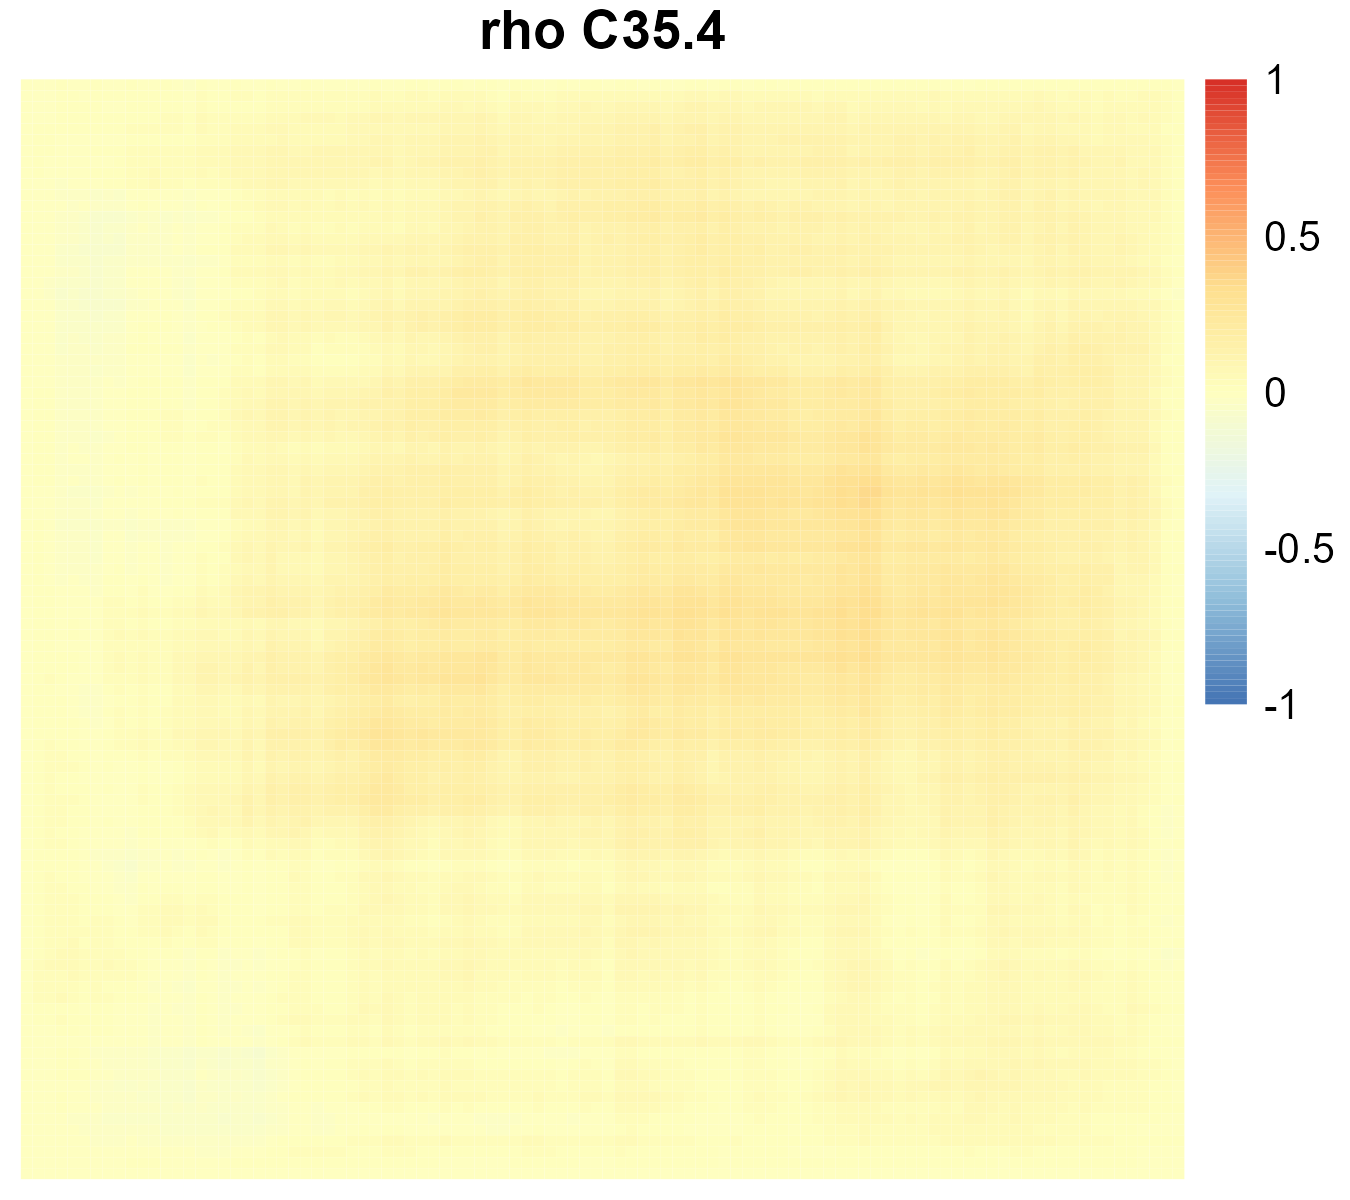
\includegraphics[width=0.33\textwidth]{4img/MujrhoC35.4.png}}
  \subfloat[$\mathscr{H}\sigma_{C_{35|4}}$]{
   \label{C35.4sigma}
    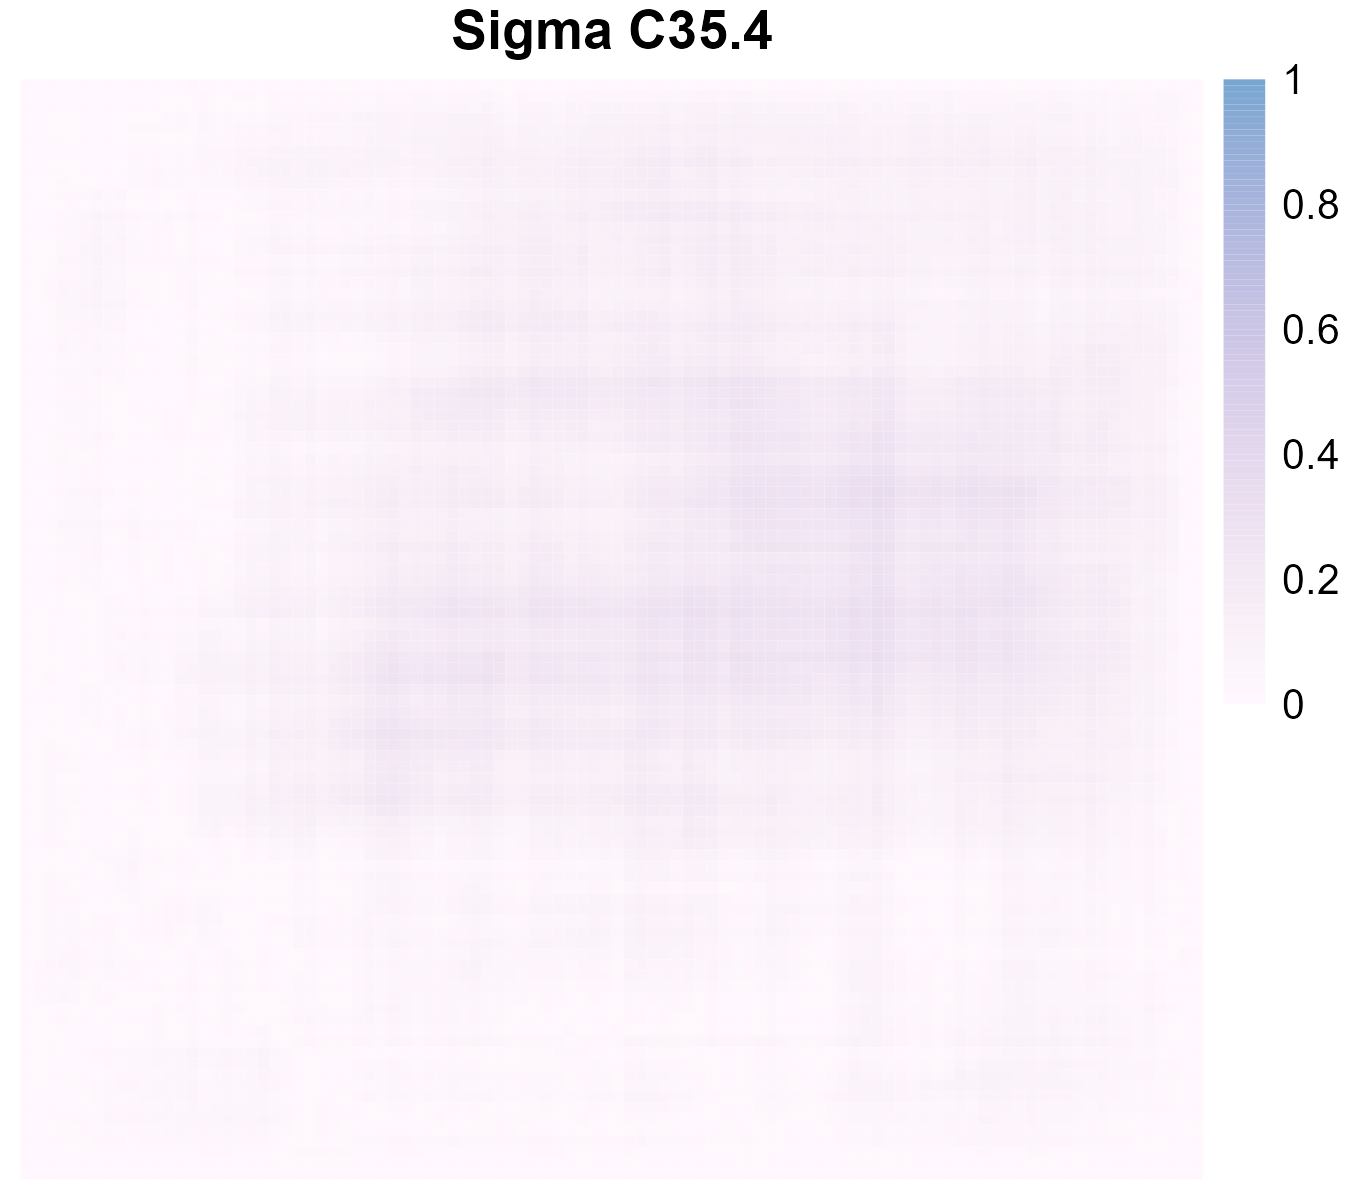
\includegraphics[width=0.33\textwidth]{4img/MujsigmaC35.4.png}}
  \subfloat[$\mathscr{H}_{C_{35|4}}$]{
   \label{C35.4H}
    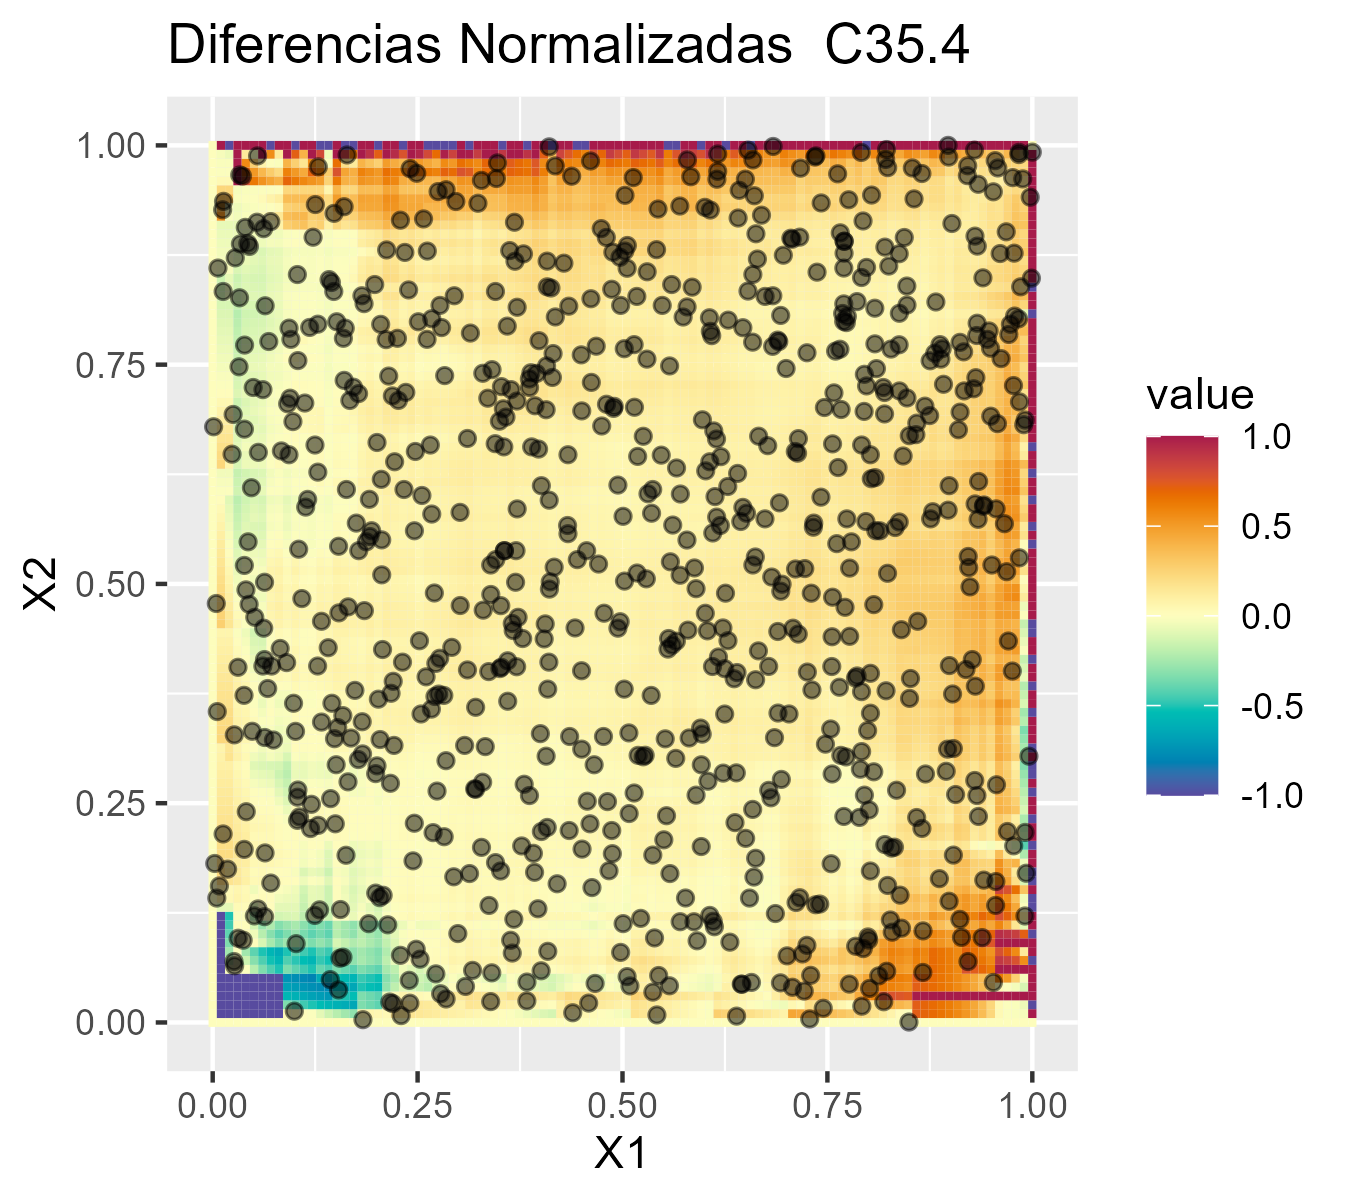
\includegraphics[width=0.33\textwidth]{4img/MujHC35.4.png}}
    \caption{Cópulas Ajustadas para Mujeres, nivel $2$.}
    \label{fig:Modelo4MujNivel2}
\end{figure}

%%%%%%%%%%%%%%%%%%%%%%%%%%%%%%%%%%%%%%%%%%%%%%%%%%

\begin{figure}[H]
 \centering
  \subfloat[$\mathscr{H}\rho_{C_{14|23}}$]{
   \label{C14.23rho}
    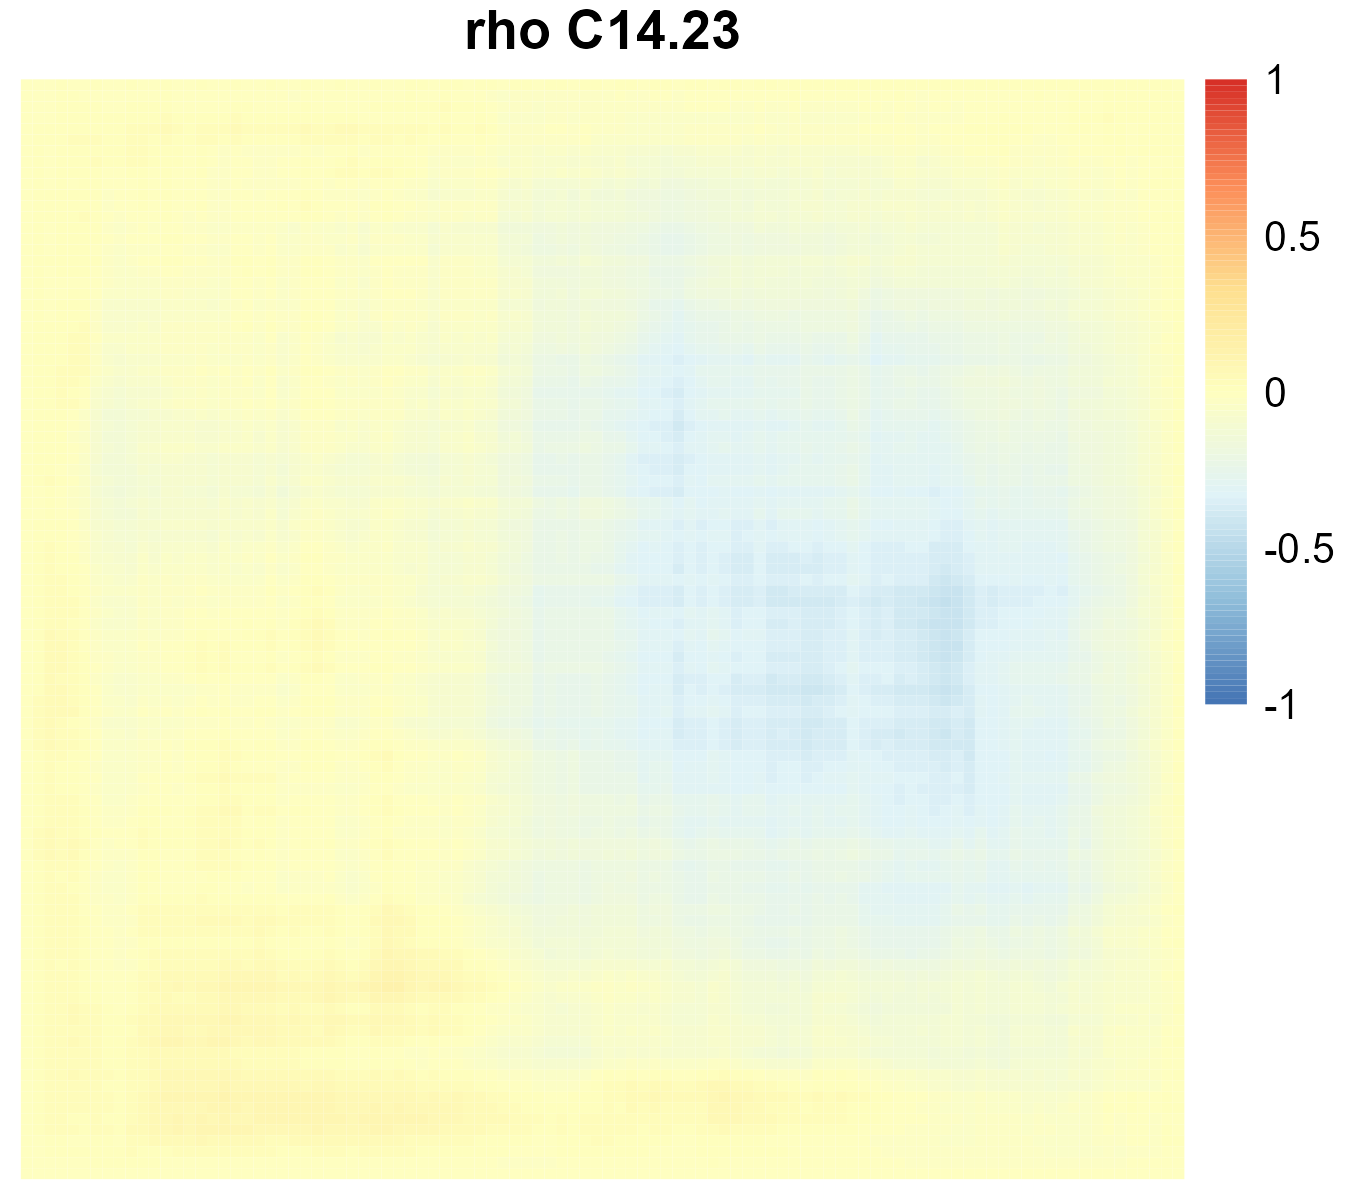
\includegraphics[width=0.3\textwidth]{4img/MujrhoC14.23.png}}
  \subfloat[$\mathscr{H}\sigma_{C_{14|23}}$]{
   \label{C14.23sigma}
    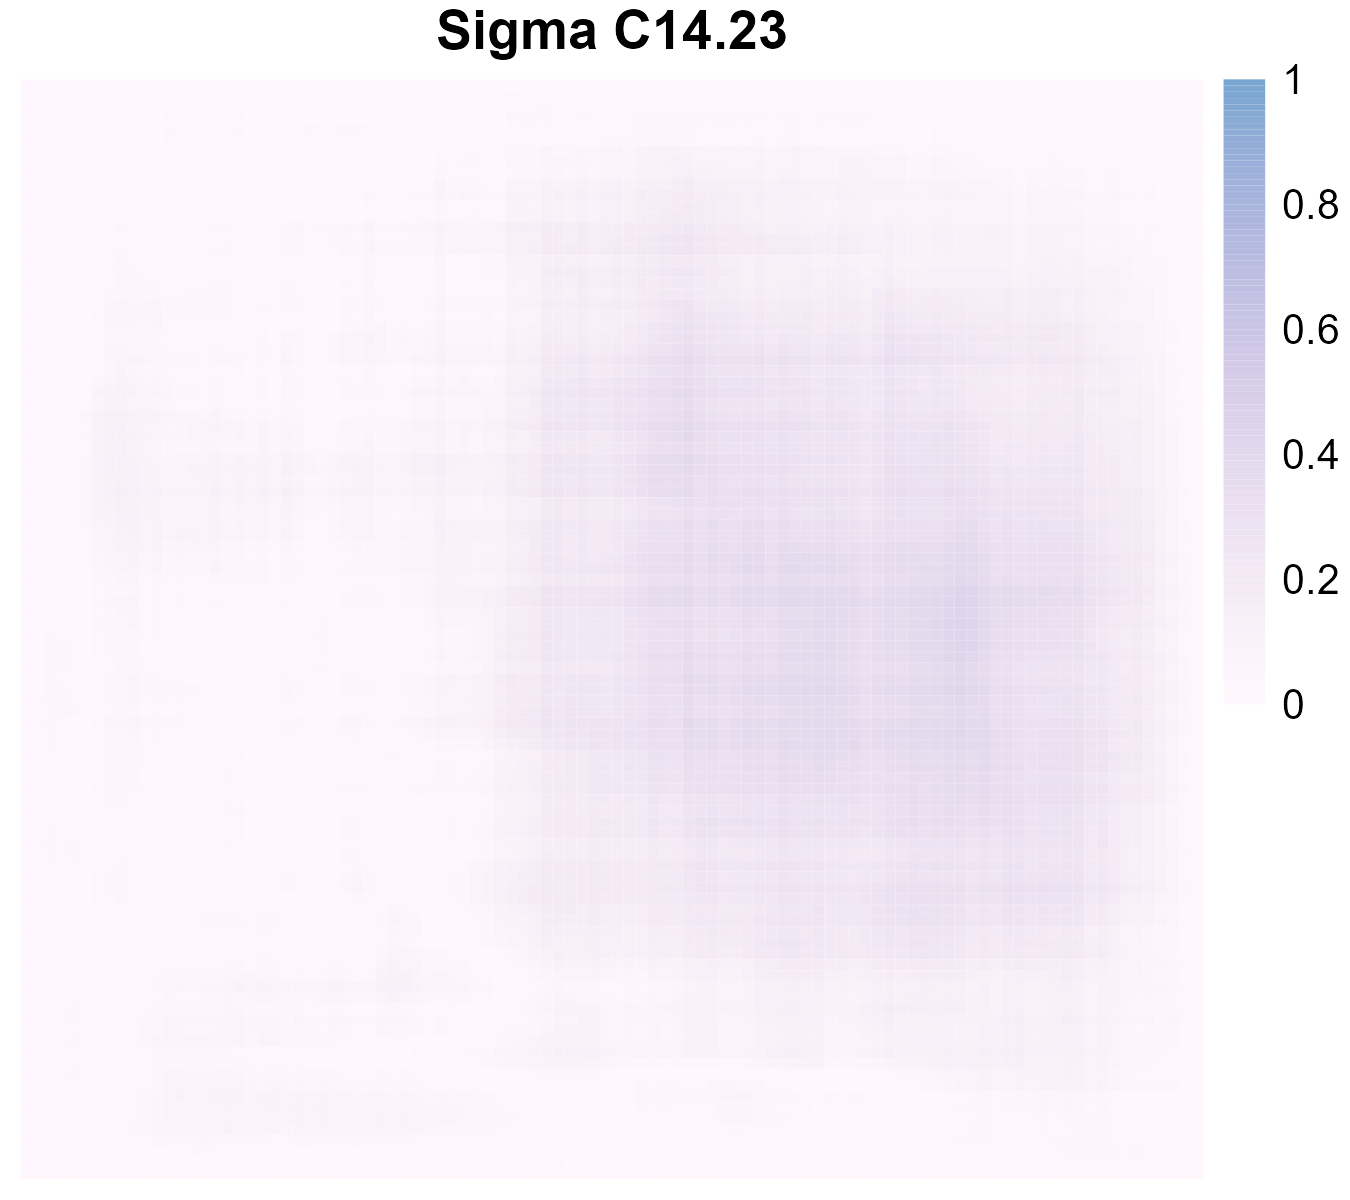
\includegraphics[width=0.3\textwidth]{4img/MujsigmaC14.23.png}}
  \subfloat[$\mathscr{H}_{C_{14|23}}$]{
   \label{C14.23H}
    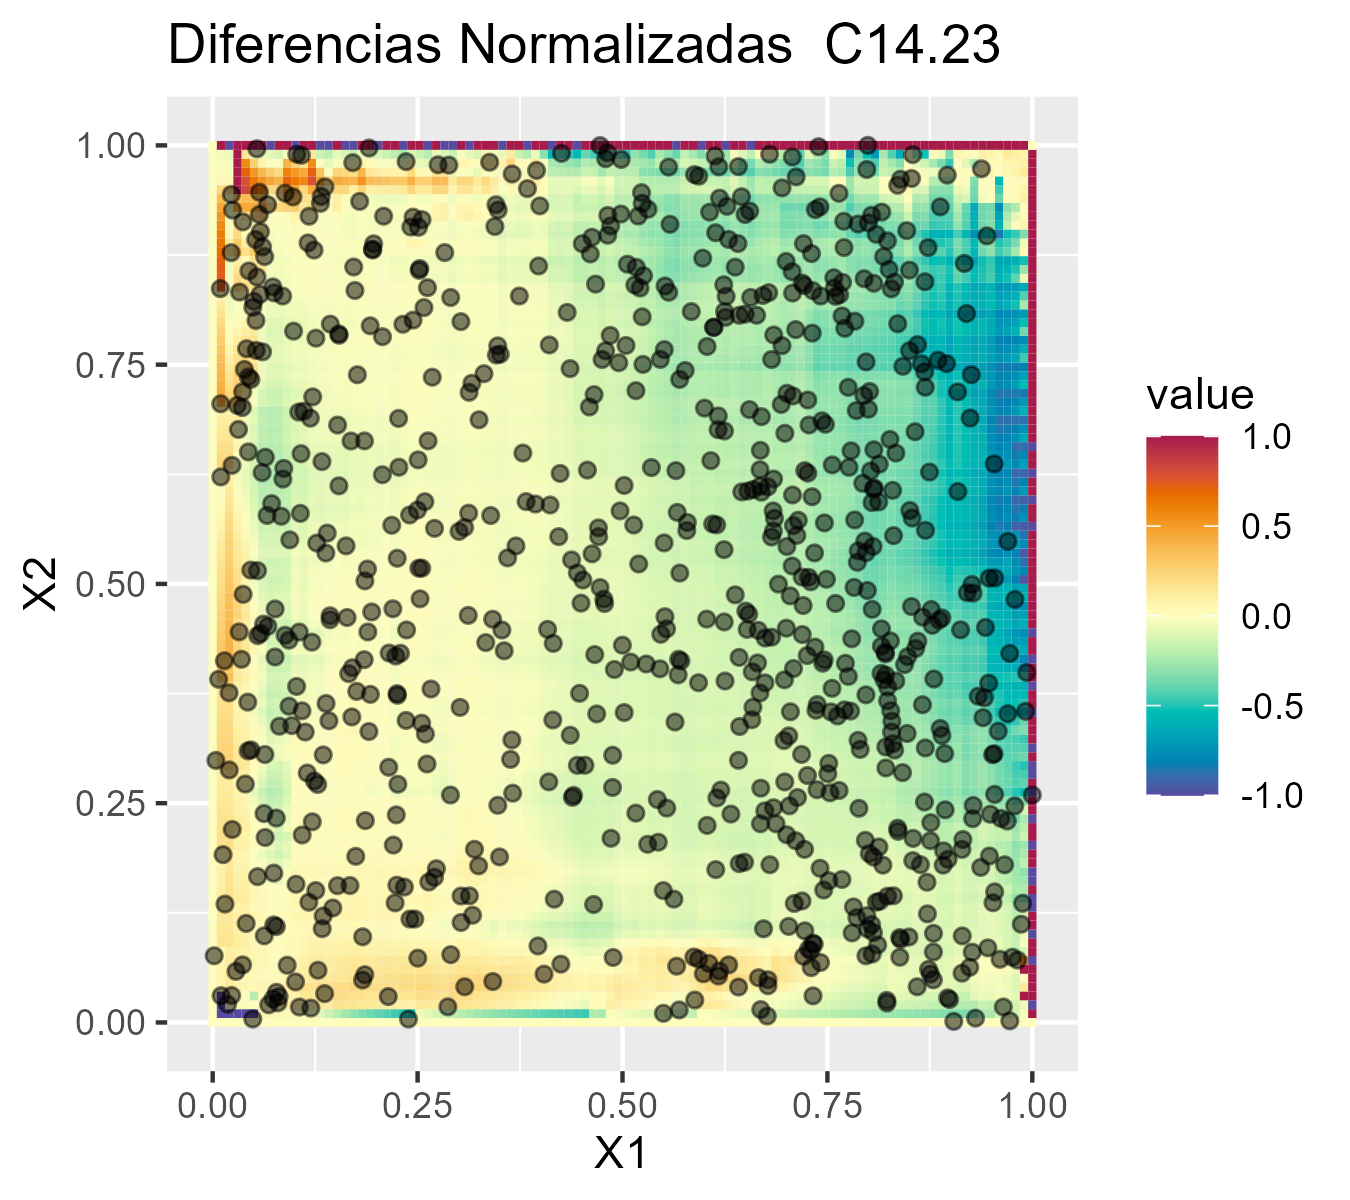
\includegraphics[width=0.3\textwidth]{4img/MujHC14.23.png}}
\end{figure}

\begin{figure}[H]
 \centering
  \subfloat[$\mathscr{H}\rho_{C_{25|34}}$]{
   \label{C25.34rho}
    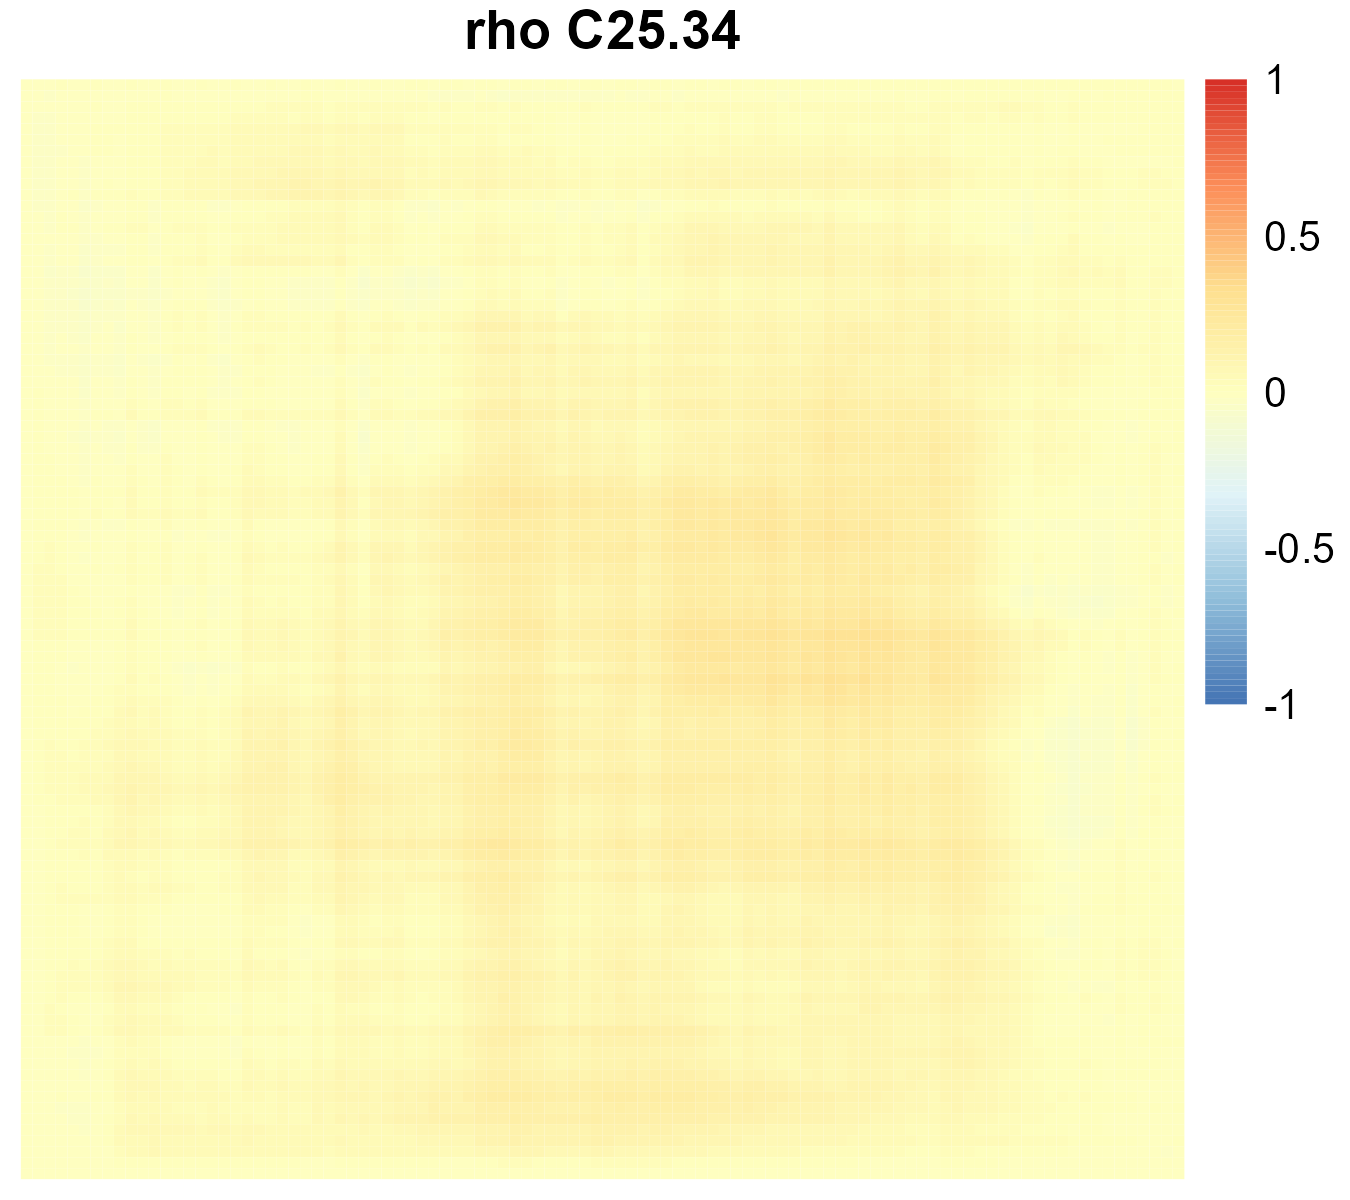
\includegraphics[width=0.3\textwidth]{4img/MujrhoC25.34.png}}
  \subfloat[$\mathscr{H}\sigma_{C_{25|34}}$]{
   \label{C25.34sigma}
    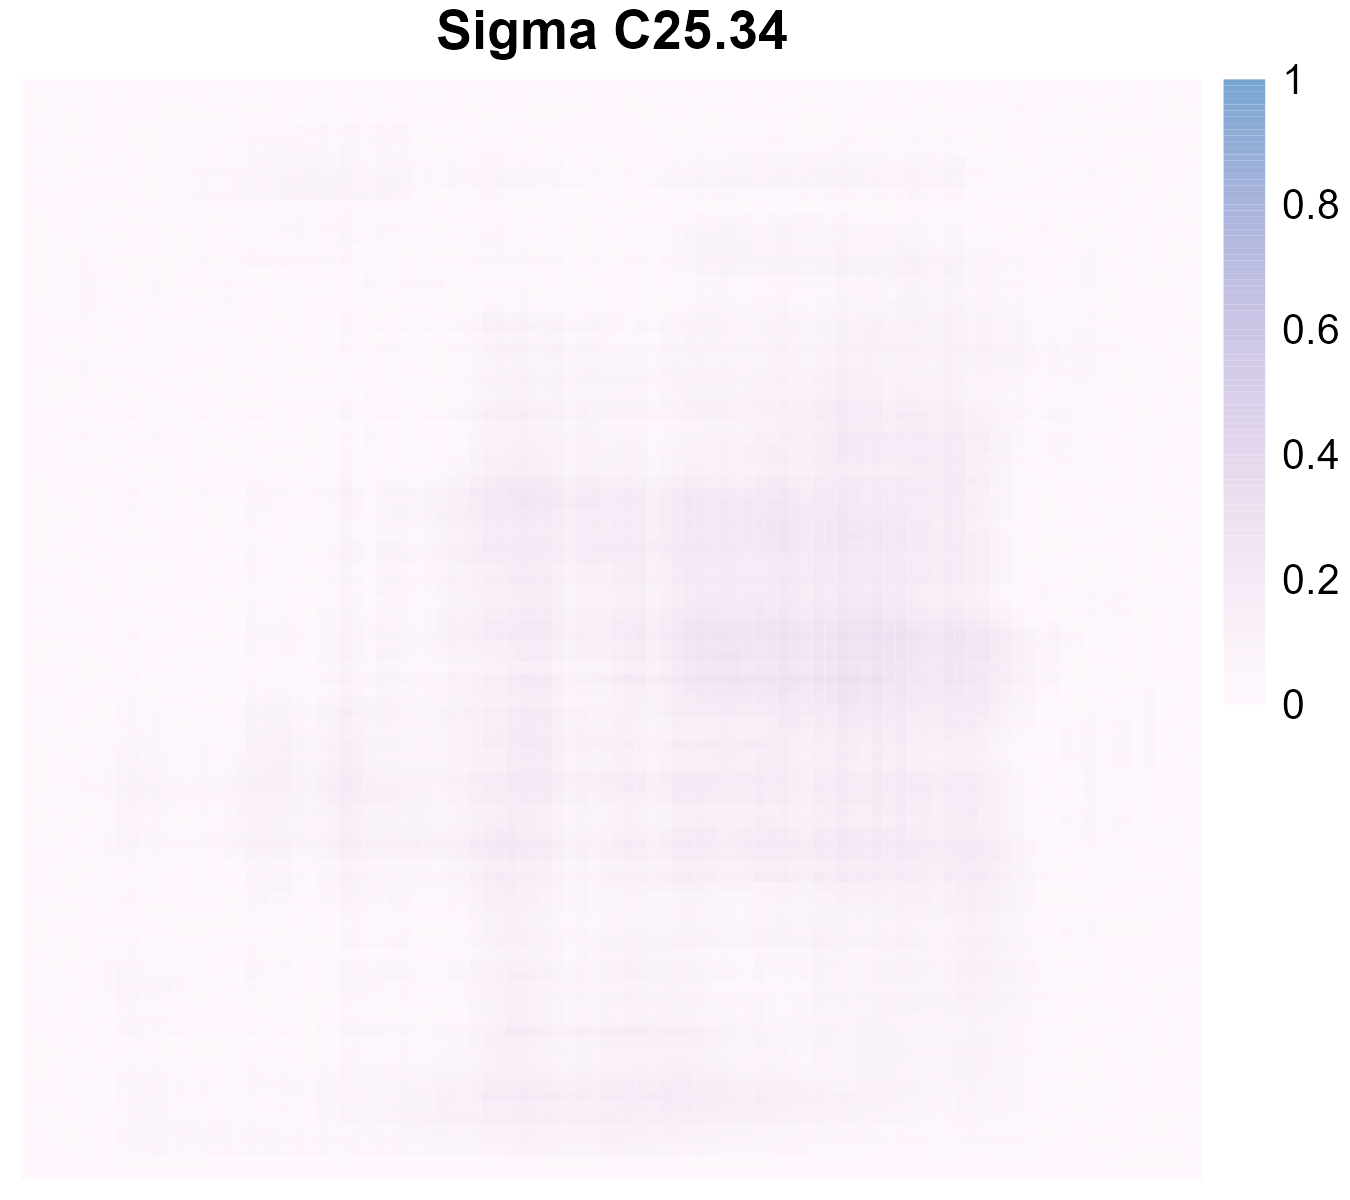
\includegraphics[width=0.3\textwidth]{4img/MujsigmaC25.34.png}}
  \subfloat[$\mathscr{H}_{C_{25|34}}$]{
   \label{C25.34H}
    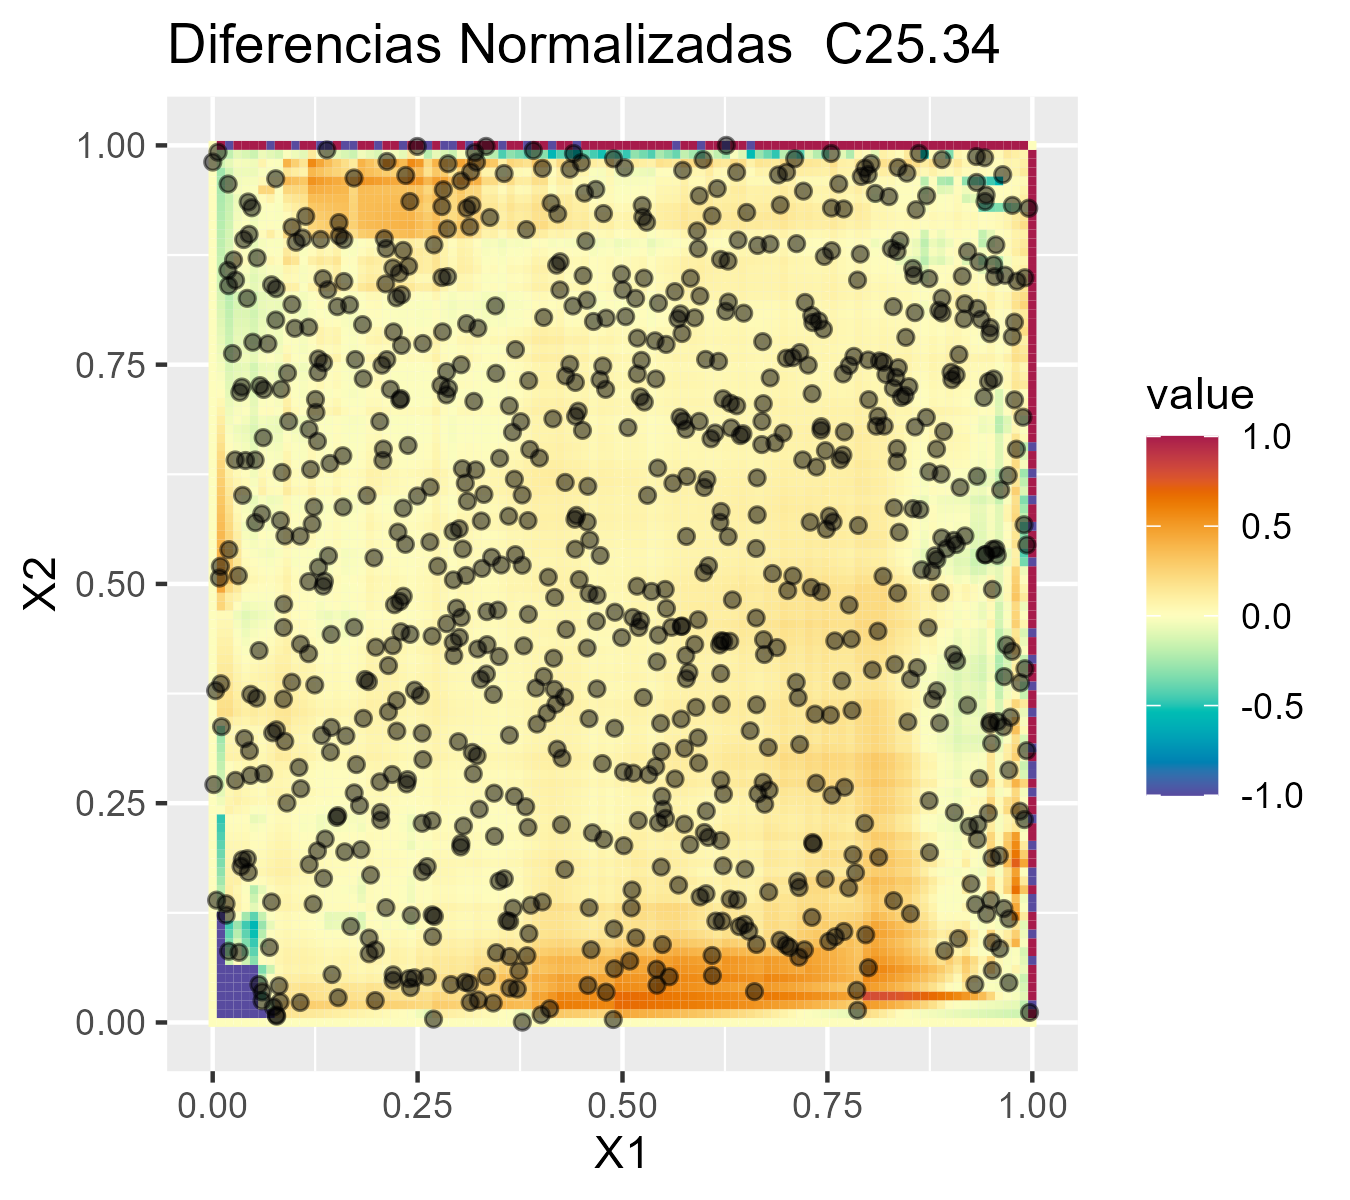
\includegraphics[width=0.3\textwidth]{4img/MujHC25.34.png}}
    \caption{Cópulas Ajustadas para Mujeres, nivel $3$.}
    \label{fig:Modelo4MujNivel3}
\end{figure}

%%%%%%%%%%%%%%%%%%%%%%%%%%%%%%%%%%%%%%%%%%%%%%%%%%

\begin{figure}[H]
 \centering
  \subfloat[$\mathscr{H}\rho_{C_{15|234}}$]{
   \label{C15.234rho}
    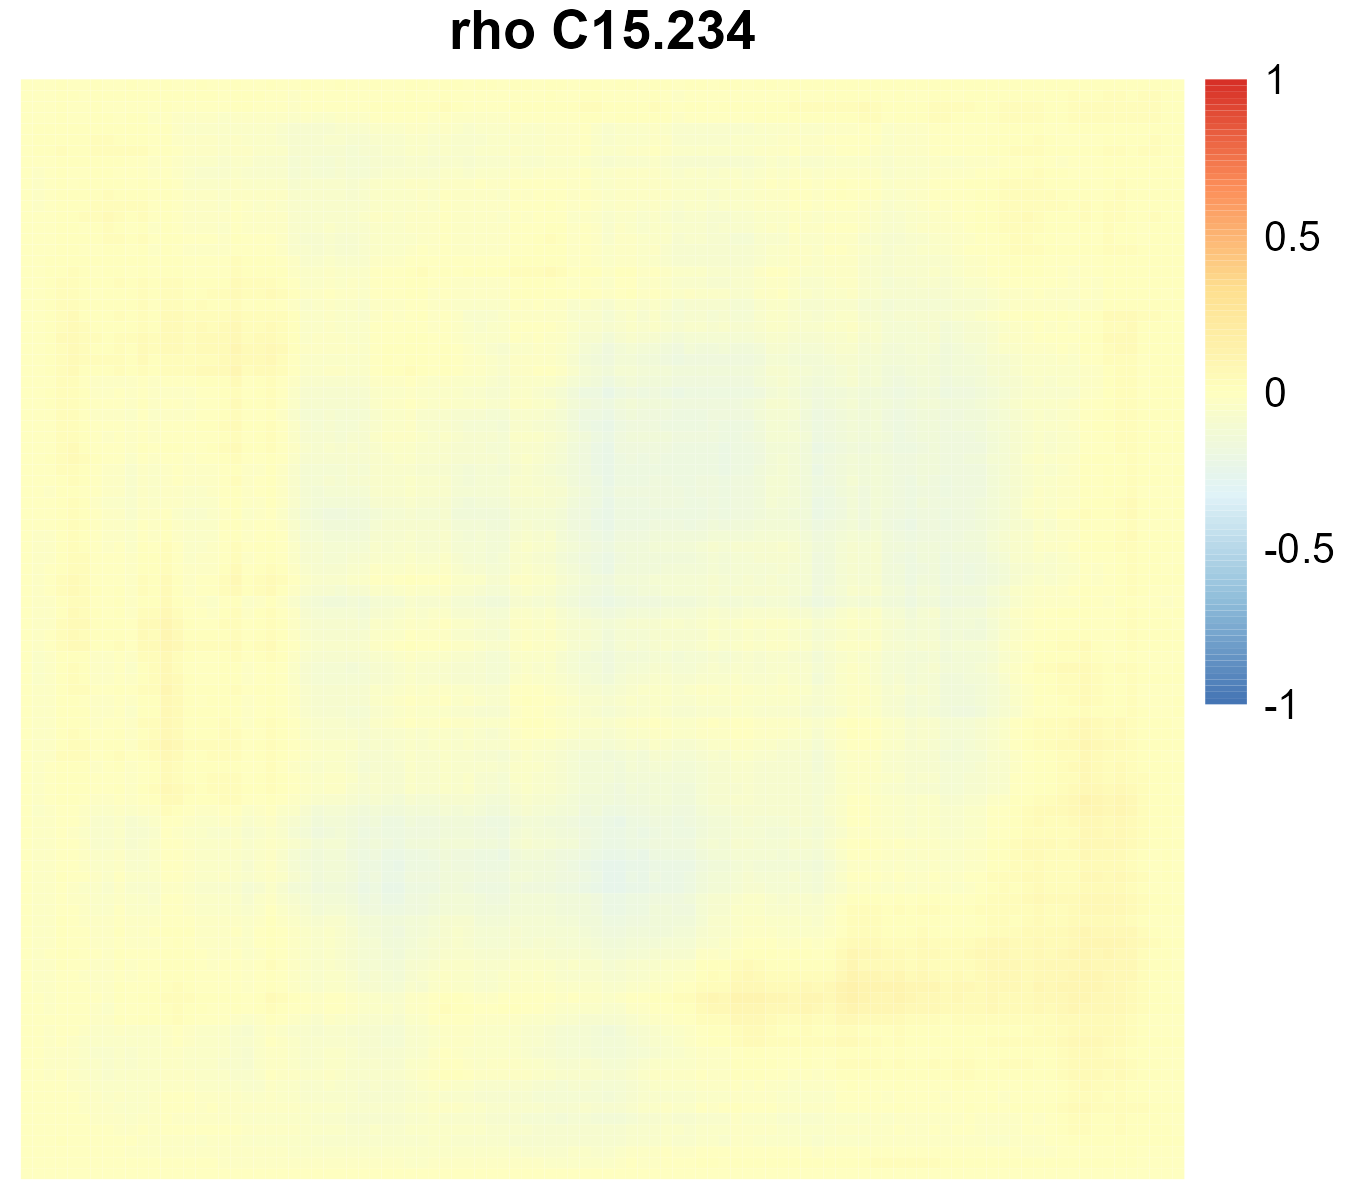
\includegraphics[width=0.3\textwidth]{4img/MujrhoC15.234.png}}
  \subfloat[$\mathscr{H}\sigma_{C_{15|234}}$]{
   \label{C15.234sigma}
    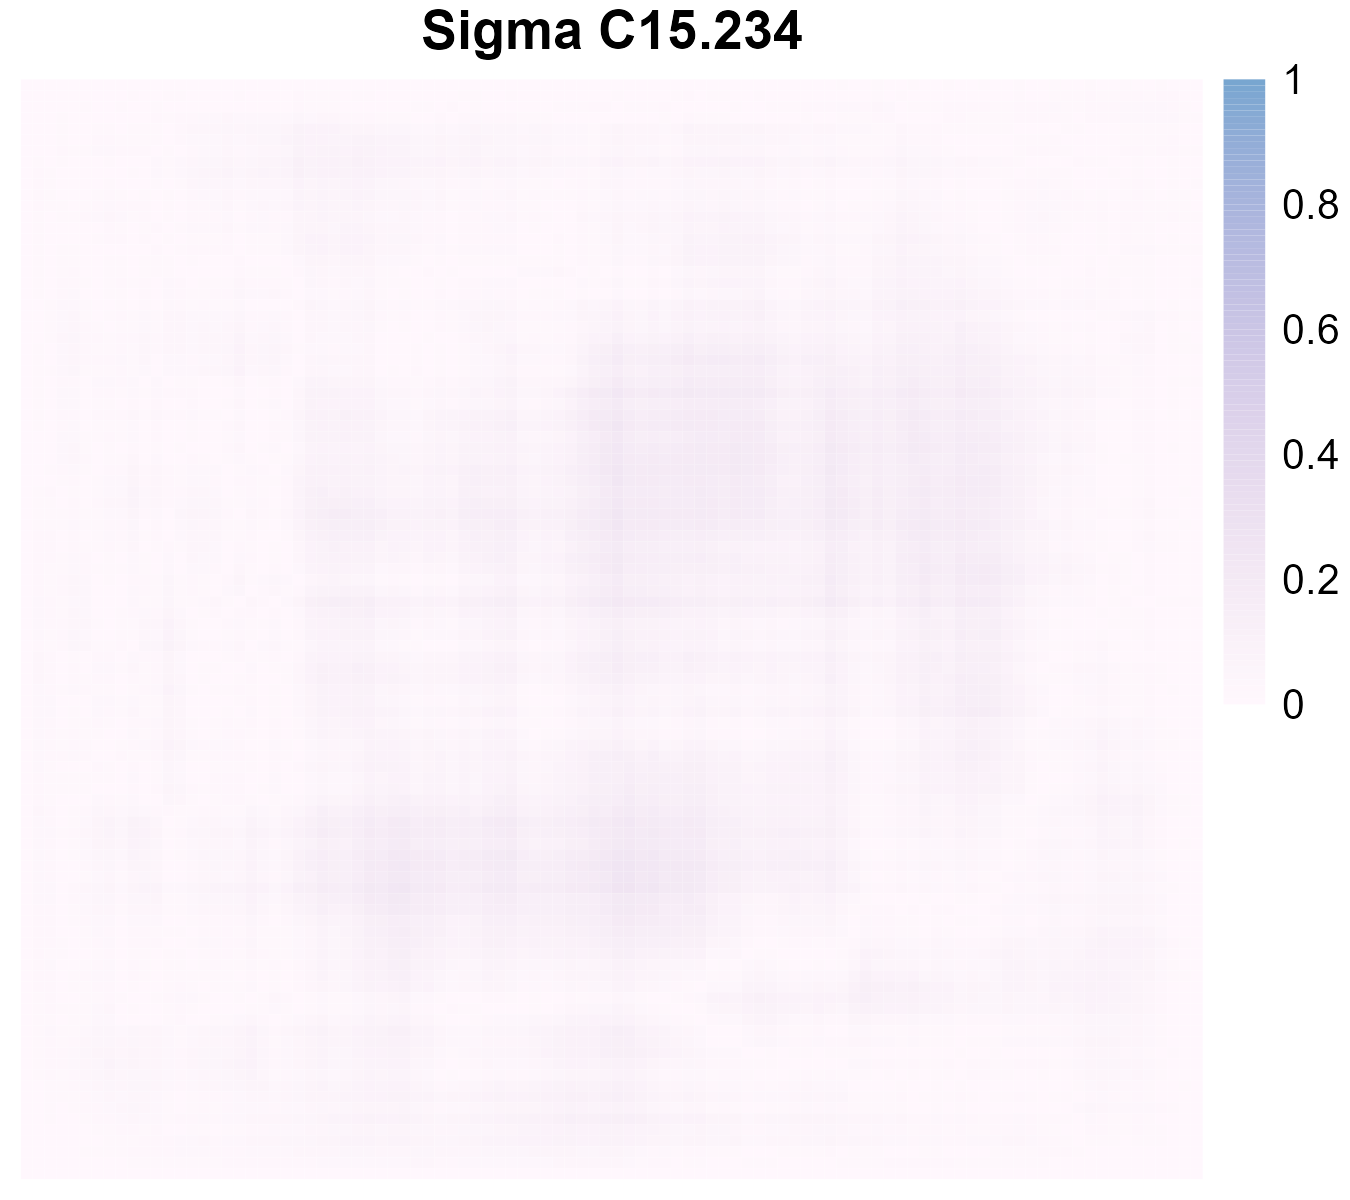
\includegraphics[width=0.3\textwidth]{4img/MujsigmaC15.234.png}}
  \subfloat[$\mathscr{H}_{C_{15|234}}$]{
   \label{C15.234H}
    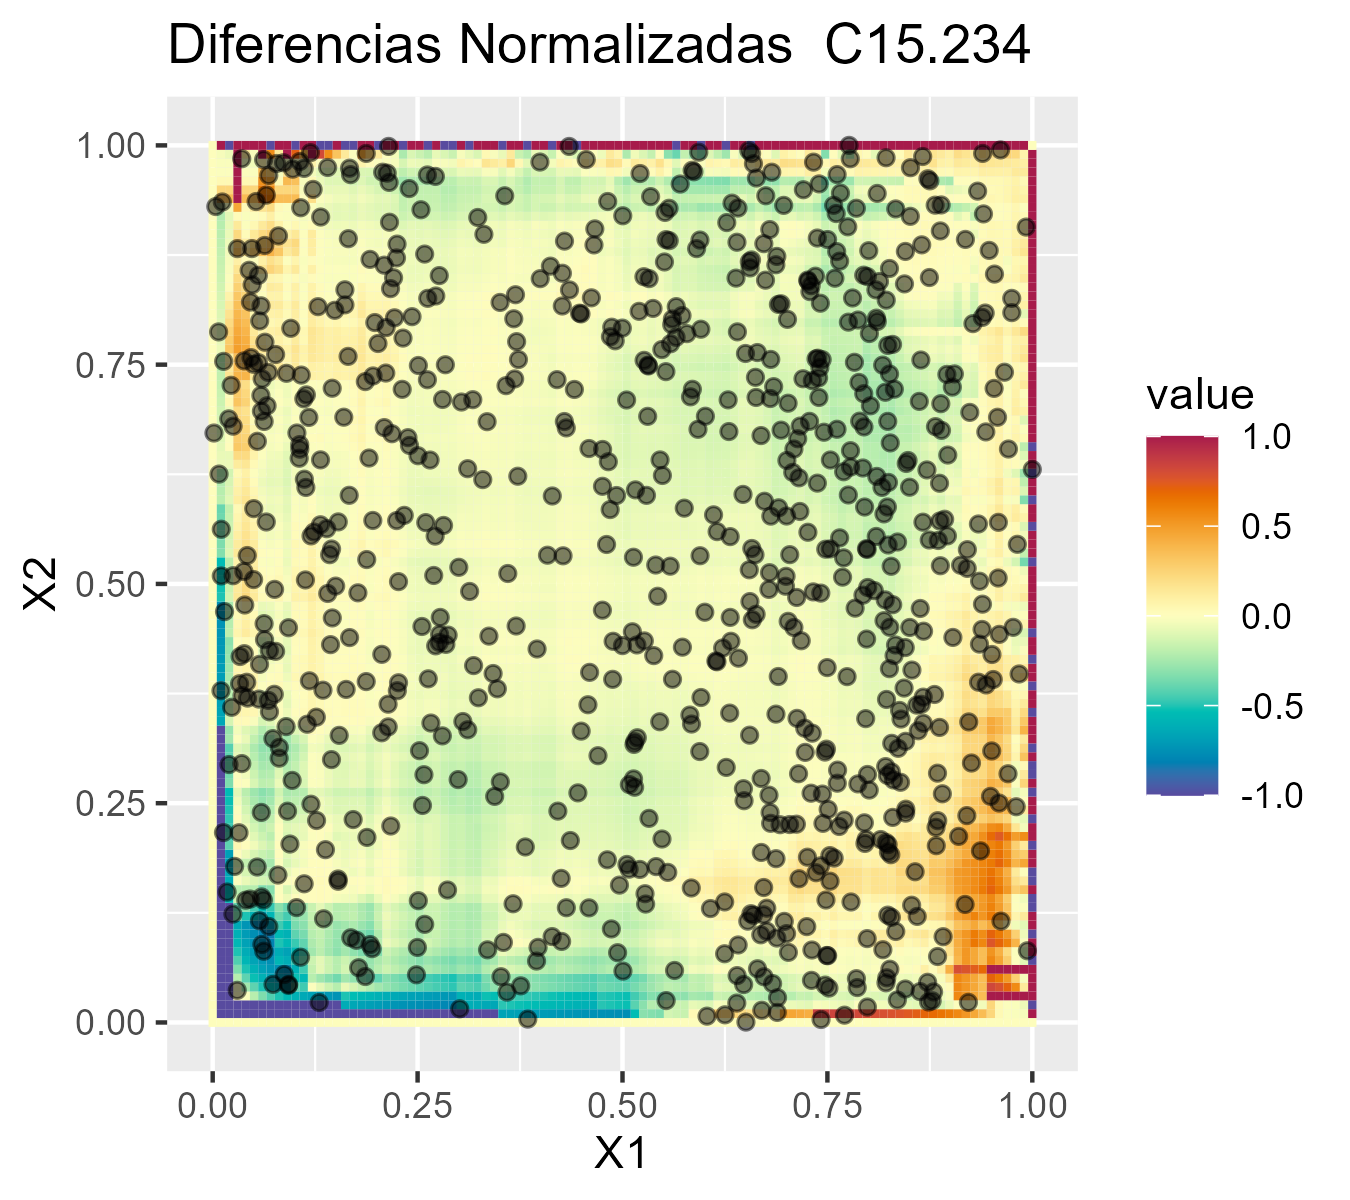
\includegraphics[width=0.3\textwidth]{4img/MujHC15.234.png}}
    \caption{Cópulas Ajustadas para Mujeres, nivel $3$.}
    \label{fig:Modelo4MujNivel4}
\end{figure}


%%%%%%%%%%%%%%%%%%%%%%%%%%%%%%%%%%%%%%%%%%%%%%%%%%
%%%%%%%%%%%%%%%%%%%%%%%%%%%%%%%%%%%%%%%%%%%%%%%%%%
\begin{figure}[H]
    \centering
    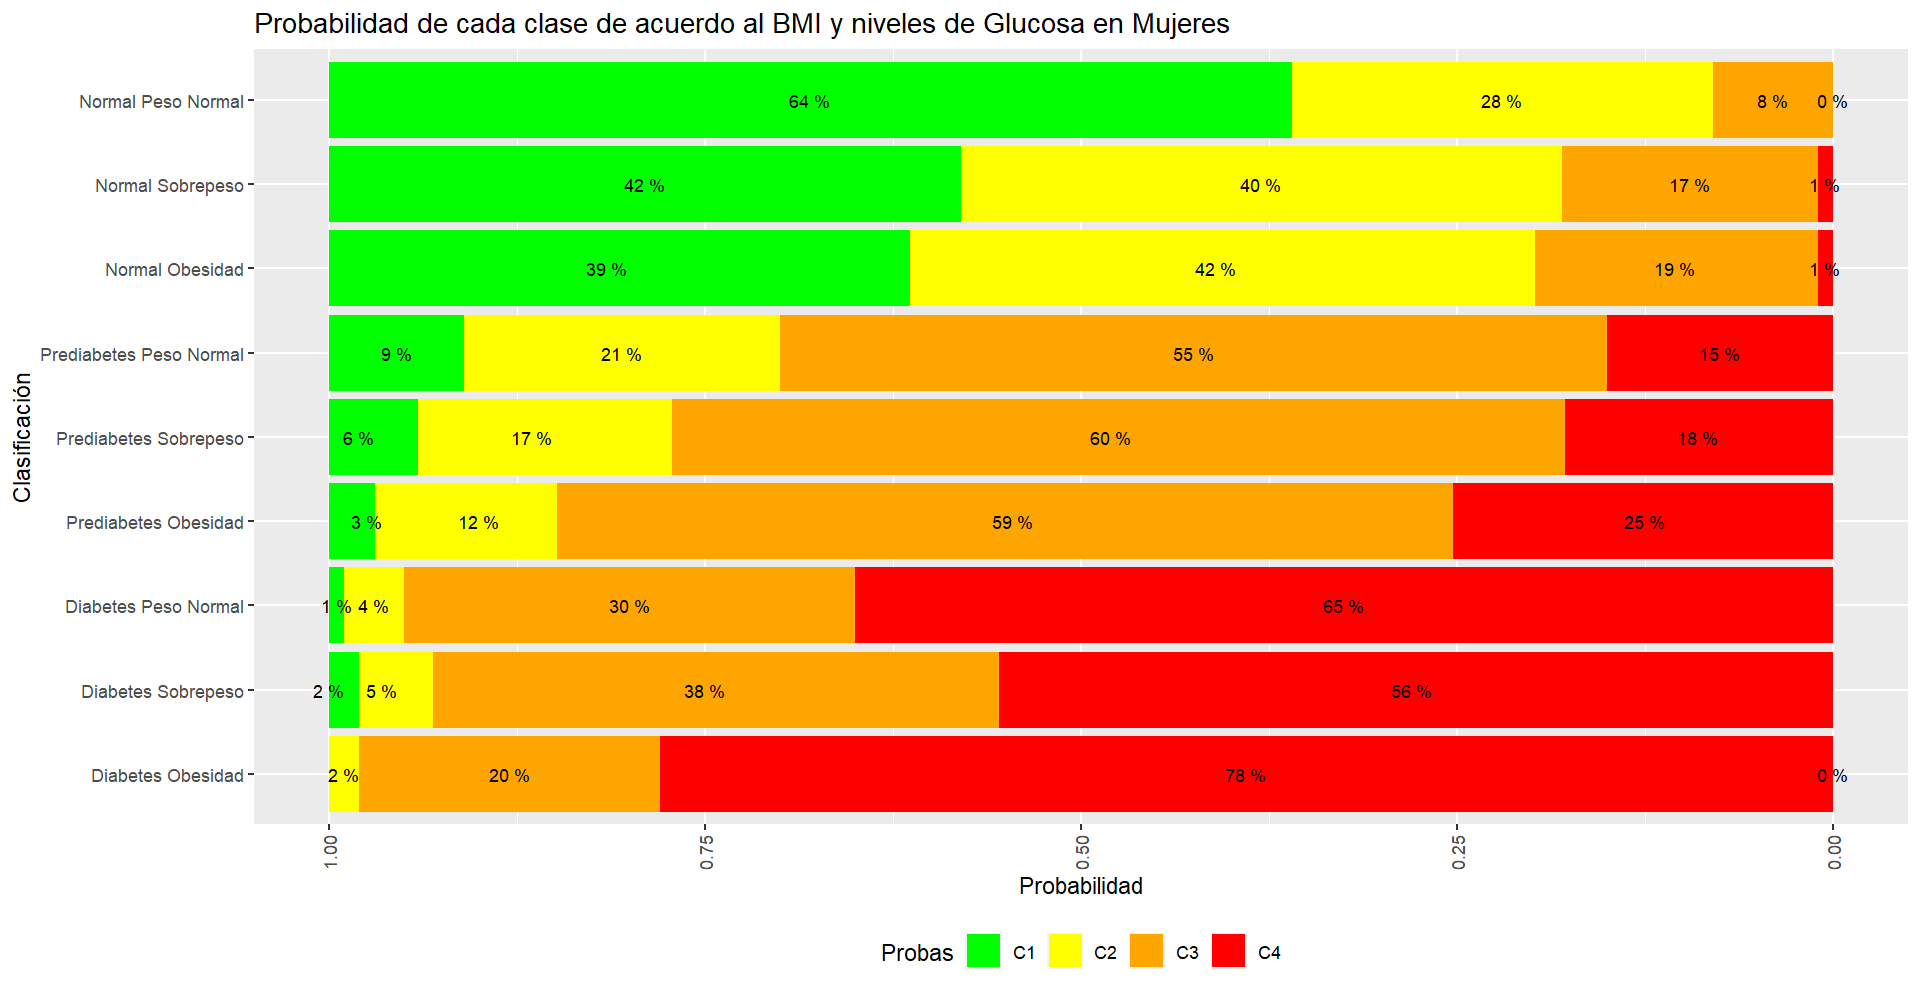
\includegraphics[height = 10 cm, width = 0.9 \textwidth]{4img/tablaM.png}
    \caption{Tabla de probabilidades de cada Clase de mujeres.}
    \label{fig:tabMujeres}
\end{figure}


%%%%%%%%%%%%%%%%%%%%%%%%%%%%%%%%%%%%%%%%%%%%%%%%%%
%%%%%%%%%%%%%%%%%%%%%%%%%%%%%%%%%%%%%%%%%%%%%%%%%%
%%%%%%%%%%%%%%%%%%%%%%%%%%%%%%%%%%%%%%%%%%%%%%%%%%
%%%%%%%%%%%%%%%%%%%%%%%%%%%%%%%%%%%%%%%%%%%%%%%%%%

\begin{landscape}
\subsection{Visualización del Modelo para Hombres}

\begin{figure}[H]
    \centering
    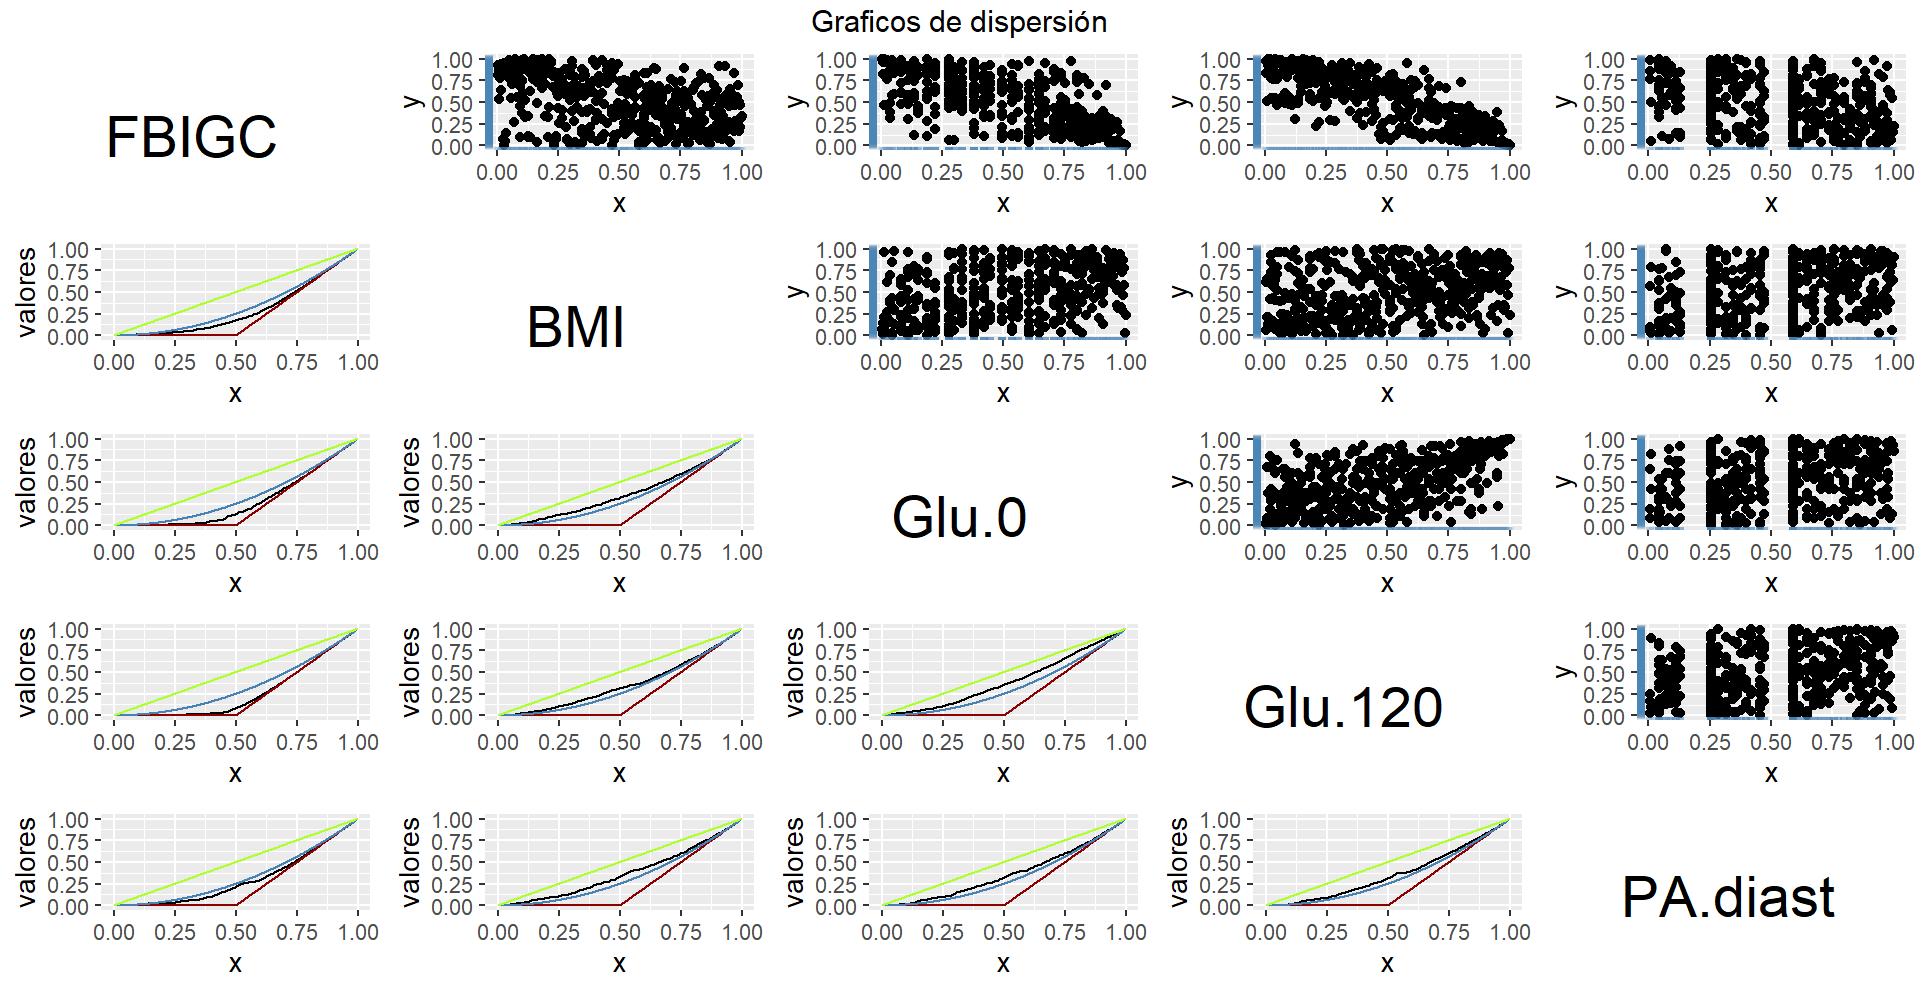
\includegraphics[height = 13.5 cm, width = 1.4 \textwidth]{4img/UdiagH.png}
    \caption{Diagonales y gráficos de dispersión en escala $u$.}
    \label{fig:diagHo}
\end{figure}
\end{landscape}

En la Figura \ref{fig:diagHo}, se presentan las diagonales de las cópulas empíricas con respecto a las diagonales de cópulas de referencia, junto con los gráficos de dispersión de las variables de individuos del género masculino. Al igual que en el caso de las mujeres, en su mayor parte, la diagonal de la cópula empírica se encuentra por debajo o por encima de la diagonal, lo que indica que las dependencias entre las variables son mayoritariamente concordantes negativas o positivas, respectivamente. También se observa la misma partición generada por la variable de presión diastólica.

\begin{figure}[H]
 \centering
  \subfloat[$\mathscr{H}\rho_{C_{12}}$]{
   \label{C12rhoH}
    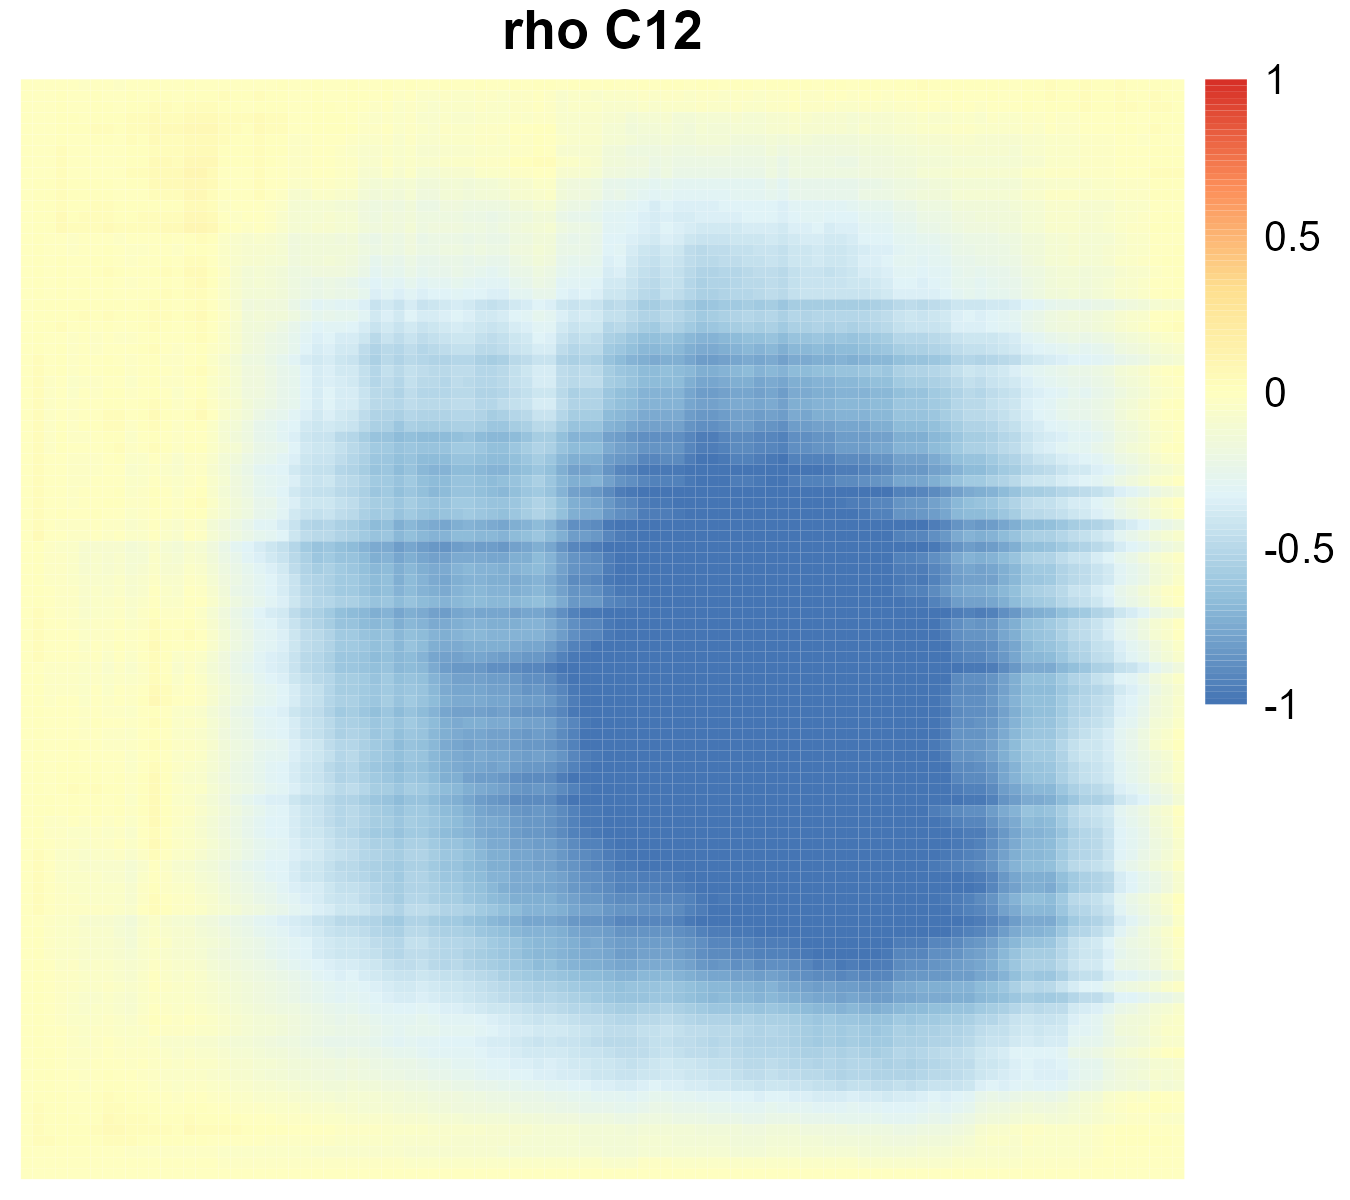
\includegraphics[width=0.3\textwidth]{4img/HomrhoC12.png}}
  \subfloat[$\mathscr{H}\sigma_{C_{12}}$]{
   \label{C12sigmaH}
    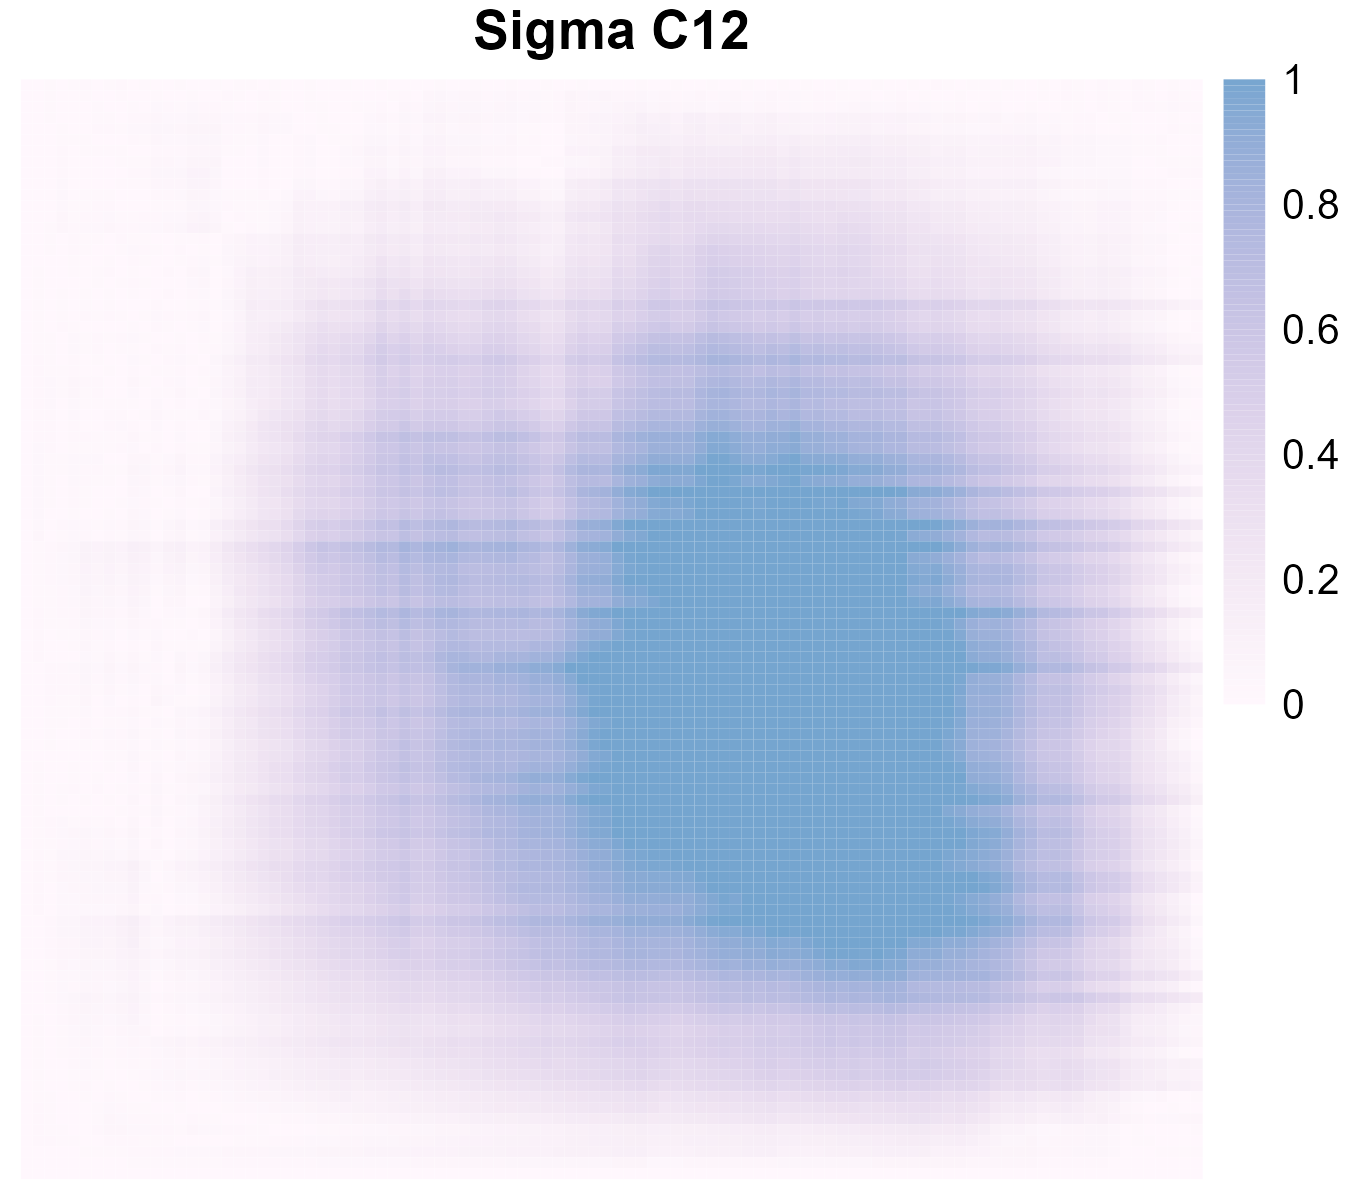
\includegraphics[width=0.3\textwidth]{4img/HomsigmaC12.png}}
  \subfloat[$\mathscr{H}_{C_{12}}$]{
   \label{C12HH}
    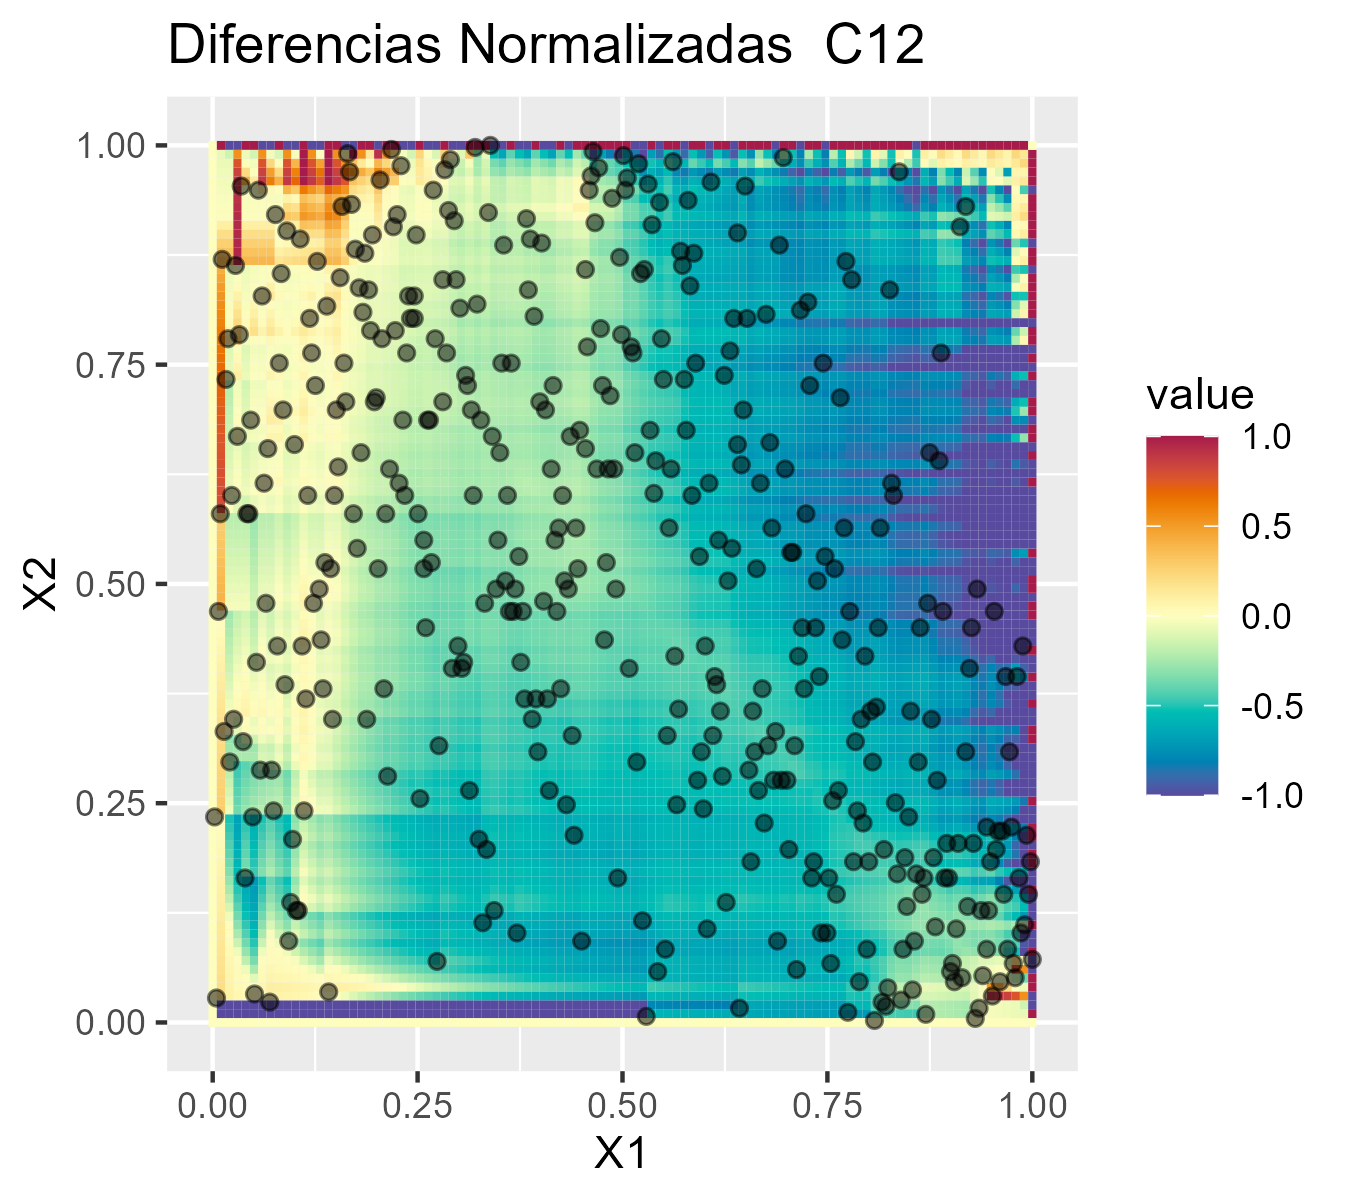
\includegraphics[width=0.3\textwidth]{4img/HomHC12.png}}
\end{figure}

\begin{figure}[H]
 \centering
  \subfloat[$\mathscr{H}\rho_{C_{23}}$]{
   \label{C23rhoH}
    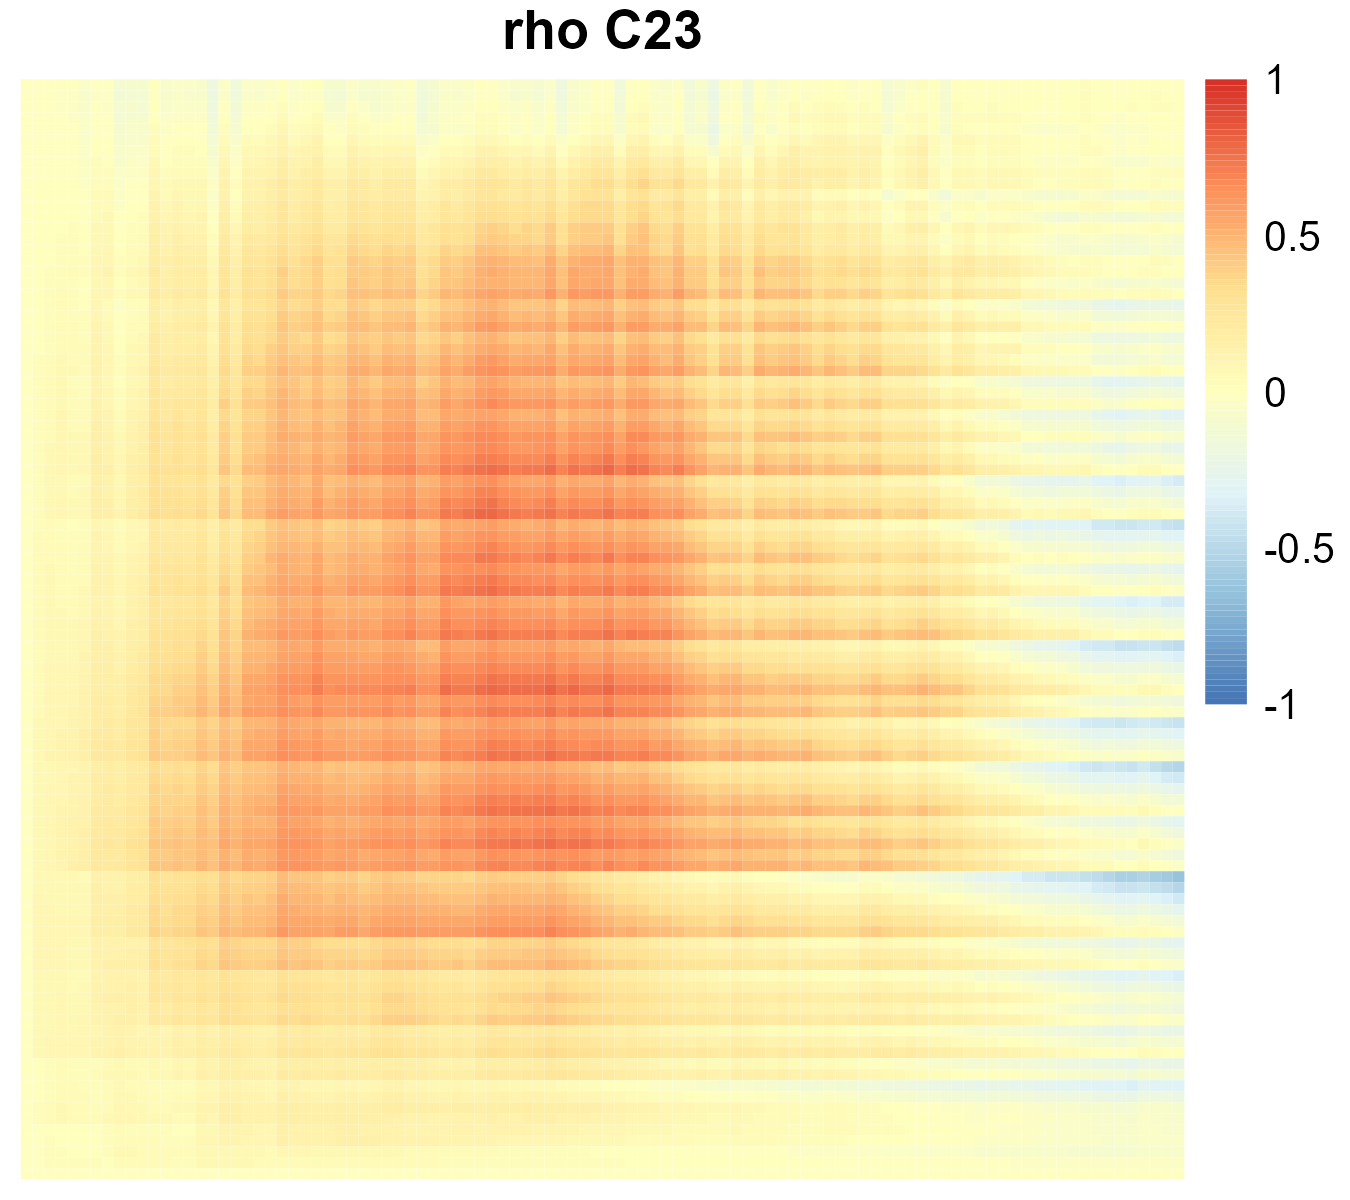
\includegraphics[width=0.3\textwidth]{4img/HomrhoC23.png}}
  \subfloat[$\mathscr{H}\sigma_{C_{23}}$]{
   \label{C23sigmaH}
    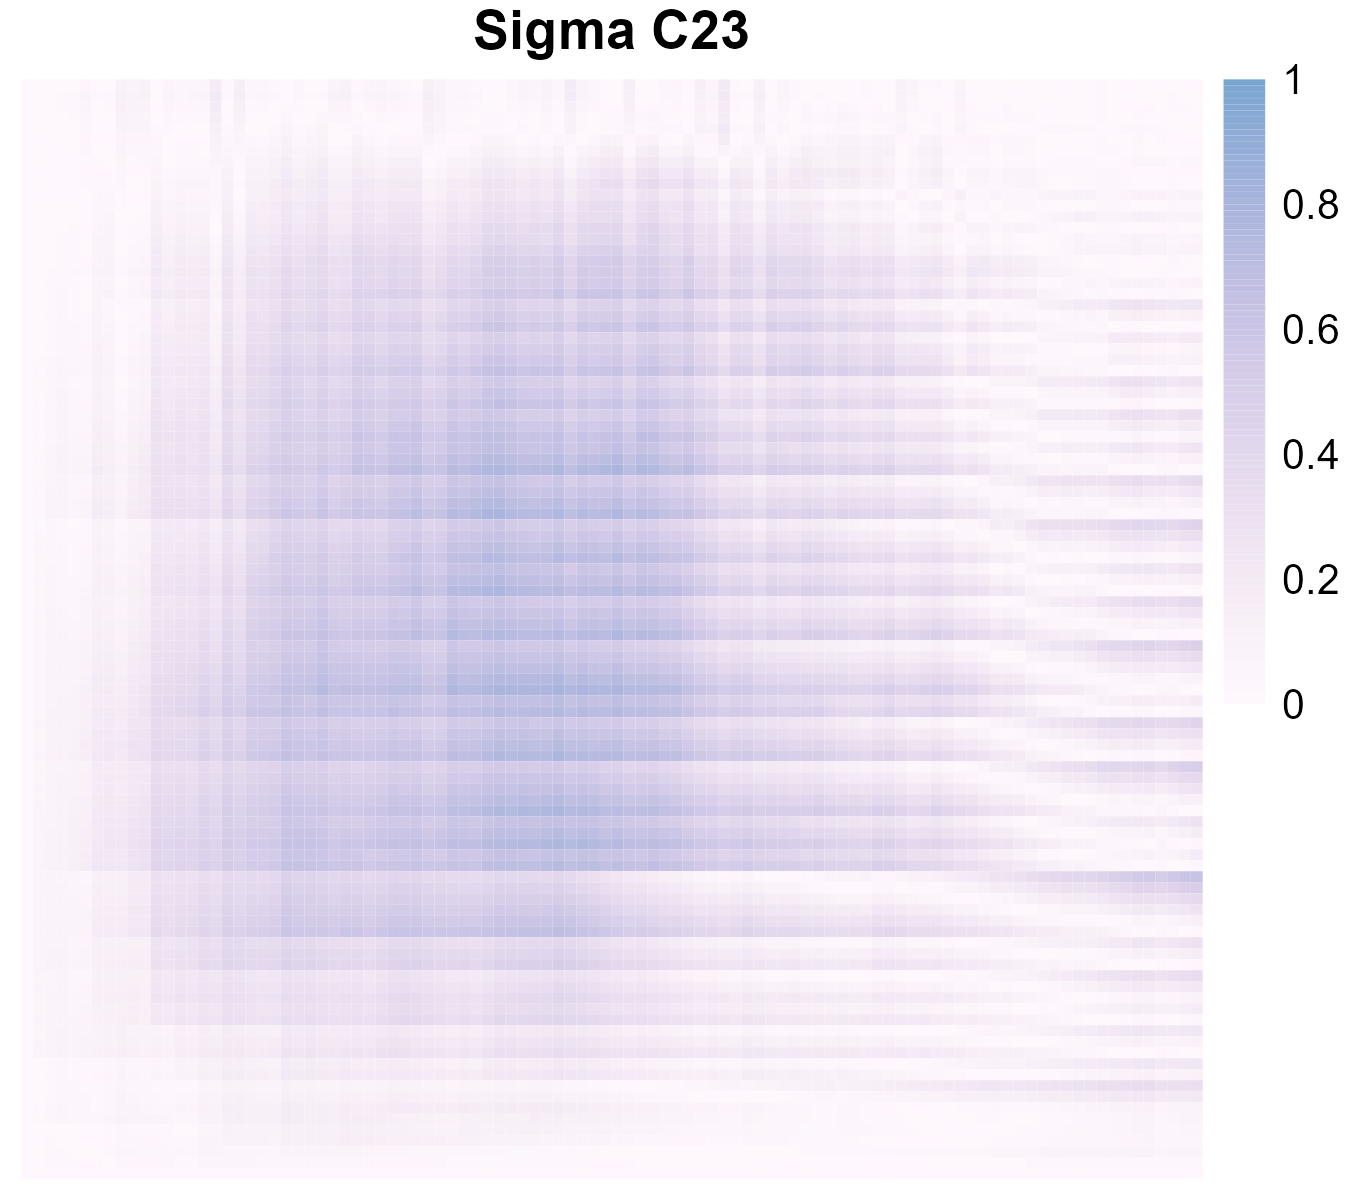
\includegraphics[width=0.3\textwidth]{4img/HomsigmaC23.png}}
  \subfloat[$\mathscr{H}_{C_{23}}$]{
   \label{C23HH}
    \includegraphics[width=0.3\textwidth]{4img/HomHC23.png}}
\end{figure}

\begin{figure}[H]
 \centering
  \subfloat[$\mathscr{H}\rho_{C_{34}}$]{
   \label{C34rhoH}
    \includegraphics[width=0.3\textwidth]{4img/HomrhoC34.png}}
  \subfloat[$\mathscr{H}\sigma_{C_{34}}$]{
   \label{C34sigmaH}
    \includegraphics[width=0.3\textwidth]{4img/HomsigmaC34.png}}
  \subfloat[$\mathscr{H}_{C_{34}}$]{
   \label{C34HH}
    \includegraphics[width=0.3\textwidth]{4img/HomHC34.png}}
\end{figure}

\begin{figure}[H]
 \centering
  \subfloat[$\mathscr{H}\rho_{C_{45}}$]{
   \label{C45rhoH}
    \includegraphics[width=0.3\textwidth]{4img/HomrhoC45.png}}
  \subfloat[$\mathscr{H}\sigma_{C_{45}}$]{
   \label{C45sigmaH}
    \includegraphics[width=0.3\textwidth]{4img/HomsigmaC45.png}}
  \subfloat[$\mathscr{H}_{C_{45}}$]{
   \label{C45HH}
    \includegraphics[width=0.3\textwidth]{4img/HomHC45.png}}
    \caption{Cópulas Ajustadas para hombres, nivel $1$.}
    \label{fig:Modelo4HomNivel1}
\end{figure}

%%%%%%%%%%%%%%%%%%%%%%%%%%%%%%%%%%%%%%%%%%%%%%%%


\begin{figure}[H]
 \centering
  \subfloat[$\mathscr{H}\rho_{C_{13|2}}$]{
   \label{C13.2rhoH}
    \includegraphics[width=0.3\textwidth]{4img/HomrhoC13.2.png}}
  \subfloat[$\mathscr{H}\sigma_{C_{13|2}}$]{
   \label{C13.2sigmaH}
    \includegraphics[width=0.3\textwidth]{4img/HomsigmaC13.2.png}}
  \subfloat[$\mathscr{H}_{C_{13|2}}$]{
   \label{C13.2HH}
    \includegraphics[width=0.3\textwidth]{4img/HomHC13.2.png}}
\end{figure}

\begin{figure}[H]
 \centering
  \subfloat[$\mathscr{H}\rho_{C_{24|3}}$]{
   \label{C24.3rhoH}
    \includegraphics[width=0.3\textwidth]{4img/HomrhoC24.3.png}}
  \subfloat[$\mathscr{H}\sigma_{C_{24|3}}$]{
   \label{C24.3sigmaH}
    \includegraphics[width=0.3\textwidth]{4img/HomsigmaC24.3.png}}
  \subfloat[$\mathscr{H}_{C_{24|3}}$]{
   \label{C24.3HH}
    \includegraphics[width=0.3\textwidth]{4img/HomHC24.3.png}}
\end{figure}

\begin{figure}[H]
 \centering
  \subfloat[$\mathscr{H}\rho_{C_{35|4}}$]{
   \label{C35.4rhoH}
    \includegraphics[width=0.3\textwidth]{4img/HomrhoC35.4.png}}
  \subfloat[$\mathscr{H}\sigma_{C_{35|4}}$]{
   \label{C35.4sigmaH}
    \includegraphics[width=0.3\textwidth]{4img/HomsigmaC35.4.png}}
  \subfloat[$\mathscr{H}_{C_{35|4}}$]{
   \label{C35.4HH}
    \includegraphics[width=0.3\textwidth]{4img/HomHC35.4.png}}
    \caption{Cópulas Ajustadas para hombres, nivel $2$.}
    \label{fig:Modelo4HomNivel2}
\end{figure}

%%%%%%%%%%%%%%%%%%%%%%%%%%%%%%%%%%%%%%%%%%%%%%%%%%

\begin{figure}[H]
 \centering
  \subfloat[$\mathscr{H}\rho_{C_{14|23}}$]{
   \label{C14.23rhoH}
    \includegraphics[width=0.3\textwidth]{4img/HomrhoC14.23.png}}
  \subfloat[$\mathscr{H}\sigma_{C_{14|23}}$]{
   \label{C14.23sigmaH}
    \includegraphics[width=0.3\textwidth]{4img/HomsigmaC14.23.png}}
  \subfloat[$\mathscr{H}_{C_{14|23}}$]{
   \label{C14.23HH}
    \includegraphics[width=0.3\textwidth]{4img/HomHC14.23.png}}
\end{figure}

\begin{figure}[H]
 \centering
  \subfloat[$\mathscr{H}\rho_{C_{25|34}}$]{
   \label{C25.34rhoH}
    \includegraphics[width=0.3\textwidth]{4img/HomrhoC25.34.png}}
  \subfloat[$\mathscr{H}\sigma_{C_{25|34}}$]{
   \label{C25.34sigmaH}
    \includegraphics[width=0.3\textwidth]{4img/HomsigmaC25.34.png}}
  \subfloat[$\mathscr{H}_{C_{25|34}}$]{
   \label{C25.34HH}
    \includegraphics[width=0.3\textwidth]{4img/HomHC25.34.png}}
    \caption{Cópulas Ajustadas para hombres, nivel $3$.}
    \label{fig:Modelo4HomNivel3}
\end{figure}

%%%%%%%%%%%%%%%%%%%%%%%%%%%%%%%%%%%%%%%%%%%%%%%%%%

\begin{figure}[H]
 \centering
  \subfloat[$\mathscr{H}\rho_{C_{15|234}}$]{
   \label{C15.234rhoH}
    \includegraphics[width=0.3\textwidth]{4img/HomrhoC15.234.png}}
  \subfloat[$\mathscr{H}\sigma_{C_{15|234}}$]{
   \label{C15.234sigmaH}
    \includegraphics[width=0.3\textwidth]{4img/HomsigmaC15.234.png}}
  \subfloat[$\mathscr{H}_{C_{15|234}}$]{
   \label{C15.234HH}
    \includegraphics[width=0.3\textwidth]{4img/HomHC15.234.png}}
    \caption{Cópulas Ajustadas para hombres, nivel $3$.}
    \label{fig:Modelo4HomNivel4}
\end{figure}

%%%%%%%%%%%%%%%%%%%%%%%%%%%%%%%%%%%%%%%%%%%%%%%%%%
%%%%%%%%%%%%%%%%%%%%%%%%%%%%%%%%%%%%%%%%%%%%%%%%%%

\begin{figure}[H]
    \centering
    \includegraphics[height = 10 cm, width = 0.9 \textwidth]{4img/tablaH.png}
    \caption{Tabla de probabilidades de cada Clase para hombres.}
    \label{fig:tabla4varHom}
\end{figure}
